% !TEX program = xelatex
\documentclass[a4paper, 14pt]{report}

% Подключение необходимых пакетов для XeLaTeX
\usepackage{fontspec}                 % Для управления шрифтами
\usepackage{polyglossia}              % Для поддержки многоязычности
\setmainlanguage{russian}             % Установка основного языка
\setotherlanguage{english}            % Дополнительный язык (если требуется)
\newfontfamily\cyrillicfonttt{Courier New} % Шрифт для моноширинного текста
% Установка основного шрифта
\setmainfont{Times New Roman}

% Пакеты для оформления документа
\usepackage{geometry}                 % Параметры полей
\usepackage{setspace}                 % Межстрочный интервал
\usepackage{titlesec}                 % Настройка заголовков
\usepackage{graphicx}                 % Вставка изображений
\usepackage{caption}                  % Настройка подписей
\usepackage{tocloft}                  % Настройка оглавления
\usepackage{hyperref}                 % Гиперссылки
\usepackage{listings}                 % Вставка исходного кода
\usepackage{xcolor}                   % Цвета для оформления кода
\usepackage{float}                    % Плавающие изображения
\usepackage{fontawesome5}             % Иконки
\usepackage{tcolorbox}                % Цветные блоки
% Настройка геометрии страницы
\geometry{
    a4paper,
    left=30mm,
    right=20mm,
    top=10mm,
    bottom=10mm,
    footskip=0mm
}

% \bibliographystyle{gost-numeric.bbx}
\usepackage[style=numeric, backend=biber]{biblatex}
\addbibresource{references.bib}

% Межстрочный интервал 1.5
\onehalfspacing

% Настройка заголовков
\titleformat{\chapter}[block]
  {\centering\bfseries\Large} % Форматирование заголовка
  {\chaptername\ \thechapter}{1em}{}

\titleformat{\section}
  {\centering\bfseries\large}
  {\thesection}{1em}{}

\titleformat{\subsection}
  {\centering\bfseries\normalsize}
  {\thesubsection}{1em}{}

% % Оглавление без точек после номеров
% \renewcommand{\cftsecleader}{\cftdotfill{\cftdotsep}}

% Подключение пакета listingsutf8 для поддержки UTF-8 в листингах
\usepackage{listingsutf8}

% Включение ссылок в оглавлении
\setcounter{tocdepth}{3}

% Настройки для листингов кода
\lstset{
    basicstyle=\ttfamily\small,
    keywordstyle=\color{blue},
    commentstyle=\color{gray},
    stringstyle=\color{red},
    numbers=left,
    numberstyle=\tiny,
    stepnumber=1,
    numbersep=5pt,
    tabsize=4,
    breaklines=true,
    breakatwhitespace=false,
    showstringspaces=false,
    frame=single
}
\makeatletter % see https://tex.stackexchange.com/a/320345
\lst@InputCatcodes
\def\lst@DefEC{%
 \lst@CCECUse \lst@ProcessLetter
  ^^80^^81^^82^^83^^84^^85^^86^^87^^88^^89^^8a^^8b^^8c^^8d^^8e^^8f%
  ^^90^^91^^92^^93^^94^^95^^96^^97^^98^^99^^9a^^9b^^9c^^9d^^9e^^9f%
  ^^a0^^a1^^a2^^a3^^a4^^a5^^a6^^a7^^a8^^a9^^aa^^ab^^ac^^ad^^ae^^af%
  ^^b0^^b1^^b2^^b3^^b4^^b5^^b6^^b7^^b8^^b9^^ba^^bb^^bc^^bd^^be^^bf%
  ^^c0^^c1^^c2^^c3^^c4^^c5^^c6^^c7^^c8^^c9^^ca^^cb^^cc^^cd^^ce^^cf%
  ^^d0^^d1^^d2^^d3^^d4^^d5^^d6^^d7^^d8^^d9^^da^^db^^dc^^dd^^de^^df%
  ^^e0^^e1^^e2^^e3^^e4^^e5^^e6^^e7^^e8^^e9^^ea^^eb^^ec^^ed^^ee^^ef%
  ^^f0^^f1^^f2^^f3^^f4^^f5^^f6^^f7^^f8^^f9^^fa^^fb^^fc^^fd^^fe^^ff%
  ^^^^20ac^^^^0153^^^^0152%
  % Basic Cyrillic alphabet coverage
  ^^^^0410^^^^0411^^^^0412^^^^0413^^^^0414^^^^0415^^^^0416^^^^0417%
  ^^^^0418^^^^0419^^^^041a^^^^041b^^^^041c^^^^041d^^^^041e^^^^041f%
  ^^^^0420^^^^0421^^^^0422^^^^0423^^^^0424^^^^0425^^^^0426^^^^0427%
  ^^^^0428^^^^0429^^^^042a^^^^042b^^^^042c^^^^042d^^^^042e^^^^042f%
  ^^^^0430^^^^0431^^^^0432^^^^0433^^^^0434^^^^0435^^^^0436^^^^0437%
  ^^^^0438^^^^0439^^^^043a^^^^043b^^^^043c^^^^043d^^^^043e^^^^043f%
  ^^^^0440^^^^0441^^^^0442^^^^0443^^^^0444^^^^0445^^^^0446^^^^0447%
  ^^^^0448^^^^0449^^^^044a^^^^044b^^^^044c^^^^044d^^^^044e^^^^044f%
  ^^^^0401^^^^0451%
  %%%
  ^^00}
\lst@RestoreCatcodes
\makeatother

\renewcommand\thesection{\arabic{section}}

\begin{document}
\newcommand{\nchapter}[1]{%
    \chapter*{#1} % Заголовок главы без нумерации
    \addcontentsline{toc}{chapter}{#1} % Добавление в оглавление
}
\newcommand{\nsubsection}[1]{%
    \subsection*{#1} % Заголовок главы без нумерации
    \addcontentsline{toc}{subsection}{#1} % Добавление в оглавление
}
\makeatletter

% Table of contents in chapter style
\renewcommand{\tableofcontents}{%
    \chapter*{\contentsname}%
    \addcontentsline{toc}{chapter}{\contentsname}%
    \@starttoc{toc}%
}
\makeatother

% Титульный лист
\begin{titlepage}
    \centering
    {\large Федеральное государственное автономное образовательное учреждение высшего образования}\\
    {\large «Национальный исследовательский университет ИТМО»}\\[0.5cm]

    {\large Факультет программной инженерии и компьютерной техники}\\[3cm]

    {\large \bfseries Лабораторная работа 1}\\[0.5cm]
    {\large \bfseries «Учетные записи и авторизация в ОС MS Windows»}\\[0.5cm]
    {\large по дисциплине}\\[0.5cm]
    {\large \bfseries «Информационная безопасность»}\\[1cm]

    {\large Вариант № \underline{1}}\\[5cm]
    \begin{flushright}
        {\large \underline{Группа: P34102}}\\[0.5cm]
        {\large \underline{Выполнил:} Лапин А.А.}\\[1cm]

        {\large \underline{Проверил:}}\\
        {\large Рыбаков С.Д.}\\[7cm]
    \end{flushright}

    {\large Санкт-Петербург}\\
    {\large 2024г.}
\end{titlepage}

\setcounter{page}{2}
% Оглавление
\tableofcontents
\newpage

% Введение
\nchapter{Цель работы}
Изучить типы учетных записей пользователей,
ознакомиться с основными принципами управления учетными записями.
Изучить основные способы авторизации пользователей.

\nchapter{Программно-аппаратные средства, используемые при выполнении работы}

Для выполнения работы было использовано ПО Parallels Desktop.

Характеристики созданной виртуальной машины:
\begin{figure}[h]
    \centering
    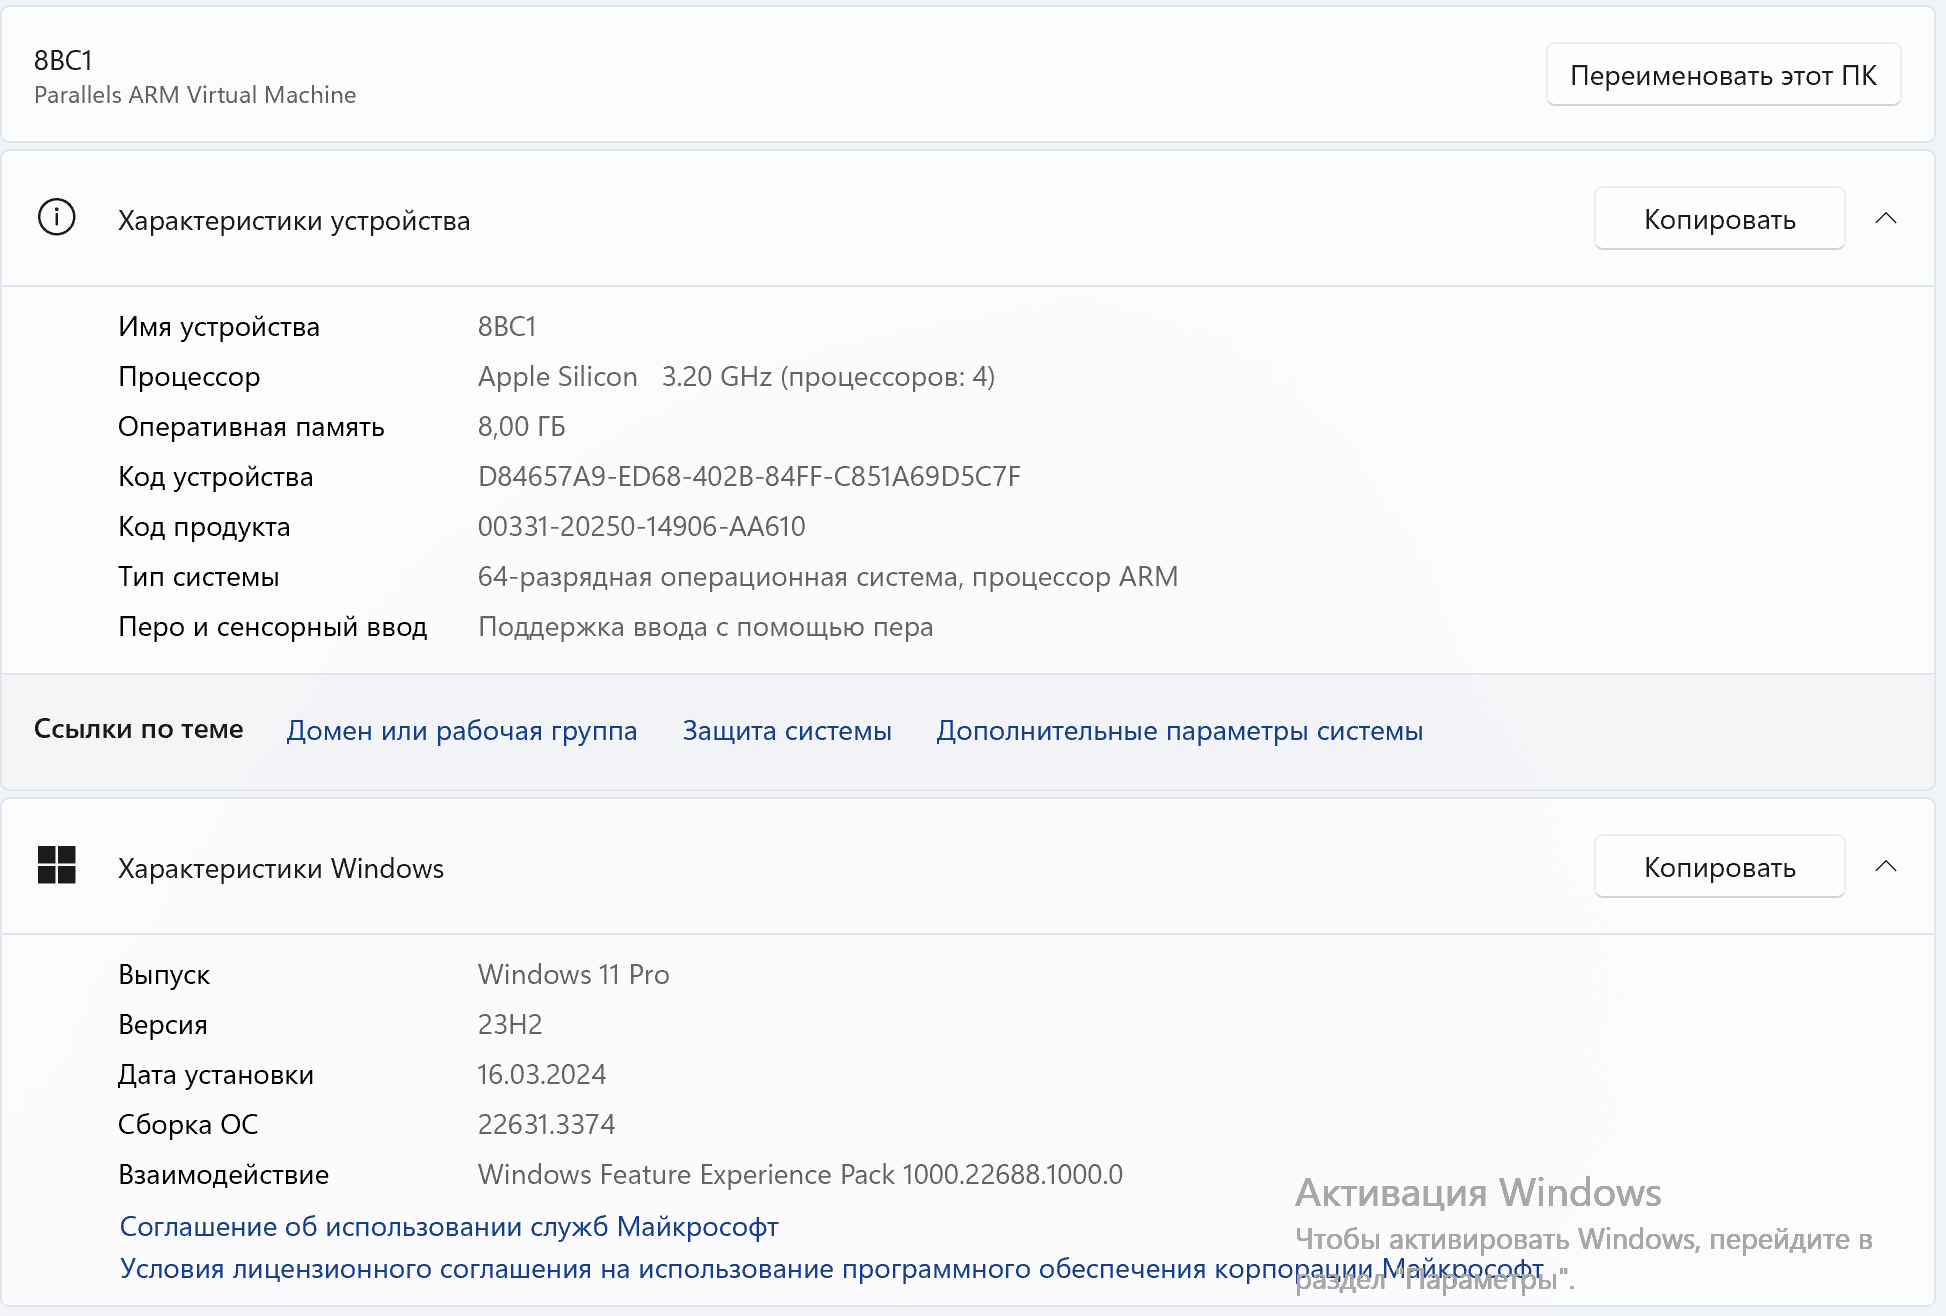
\includegraphics[width=0.8\textwidth]{../images/vm_specs.png}
    \caption{Характеристики системы}
\end{figure}
\nchapter{Основная часть}
\section{Определения}
\begin{itemize}
    \item диспетчер учетных записей (SAM);
    \item монитор безопасности (SRM);
    \item маркер доступа (access token);
    \item идентификатор безопасности (SID);
    \item привилегии пользователя;
    \item права пользователя (user rights);
    \item объект доступа;
    \item субъект доступа;
    \item олицетворение (impersonation);
    \item список контроля доступа (ACE);
    \item учетная запись;
    \item домен.
\end{itemize}
\section{Создание пользователя}


\nsubsection{Вариант 1. Создание нового пользователя в Параметрах Windows 11}
\begin{enumerate}
    \item {Откроем Параметры > Учетные записи.
          \begin{figure}[H]
              \centering
              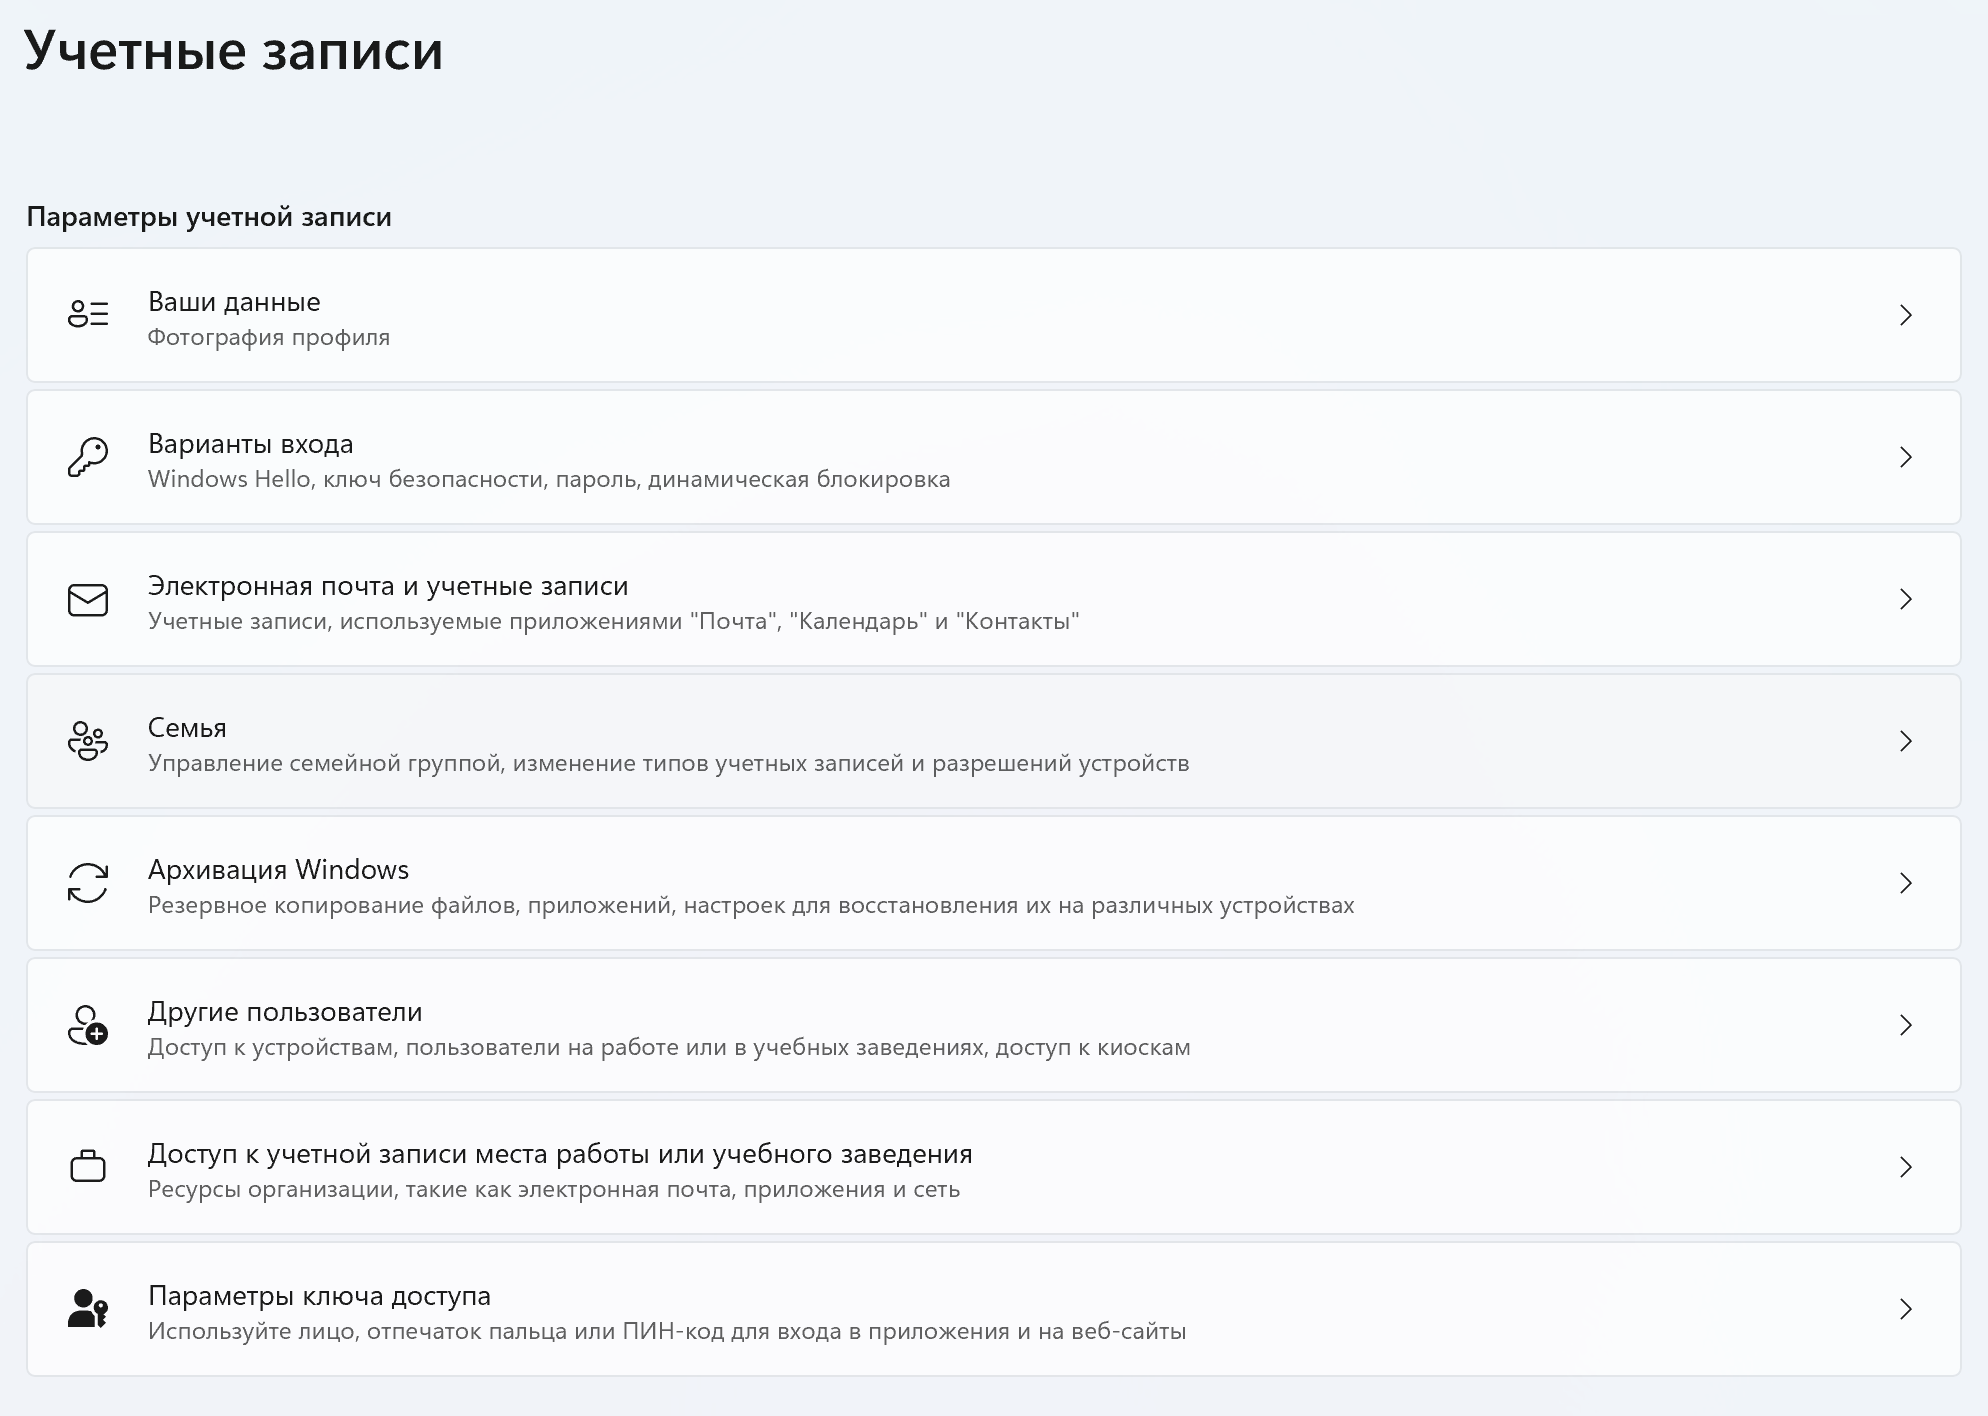
\includegraphics[width=0.8\textwidth]{../images/account_settings.png}
              \caption{Параметры учетных записей}
          \end{figure}
          }
    \item {Откроем Учетные записи > Другие пользователи > Добавить другого пользователя.
          \begin{figure}[H]
              \centering
              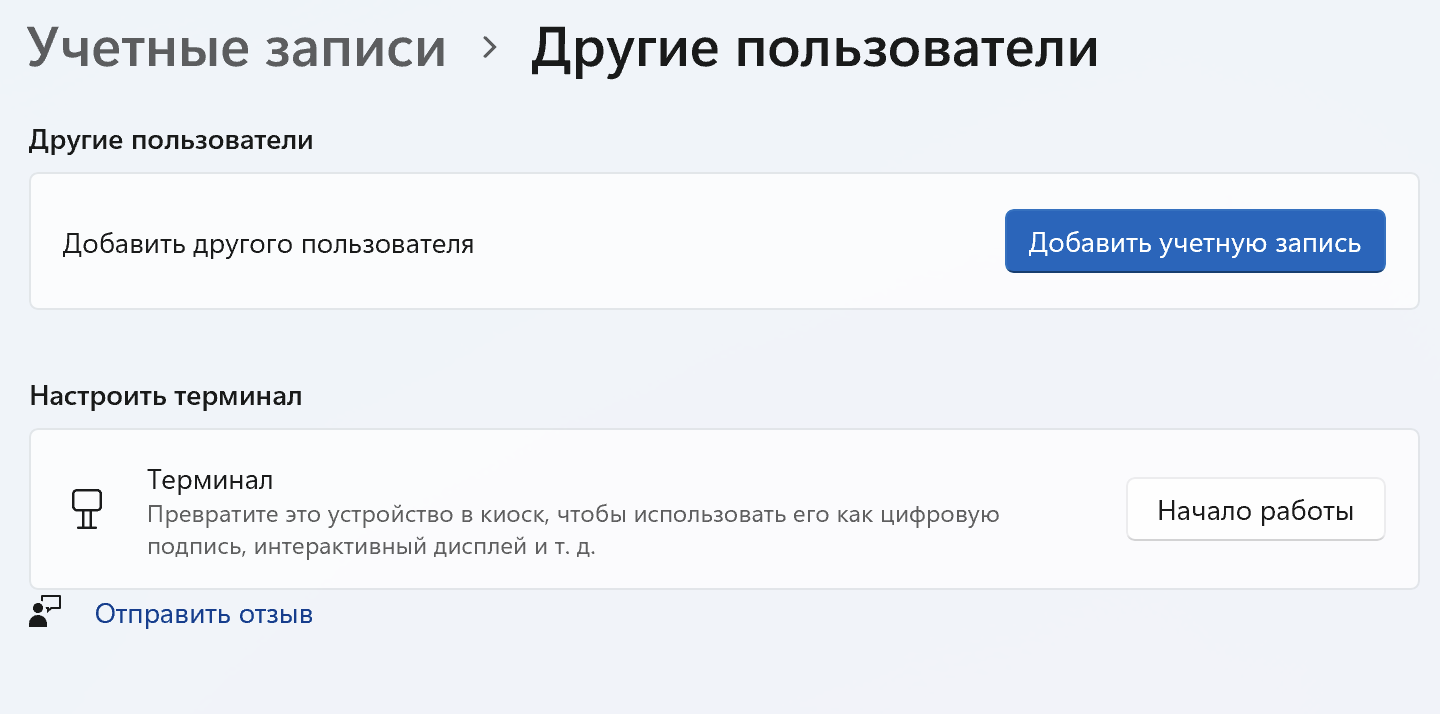
\includegraphics[width=0.8\textwidth]{../images/other_users.png}
              \caption{Другие пользователи}
          \end{figure}
          }
    \item {Выберем: «У меня нет данных для входа этого человека.»
          \begin{figure}[H]
              \centering
              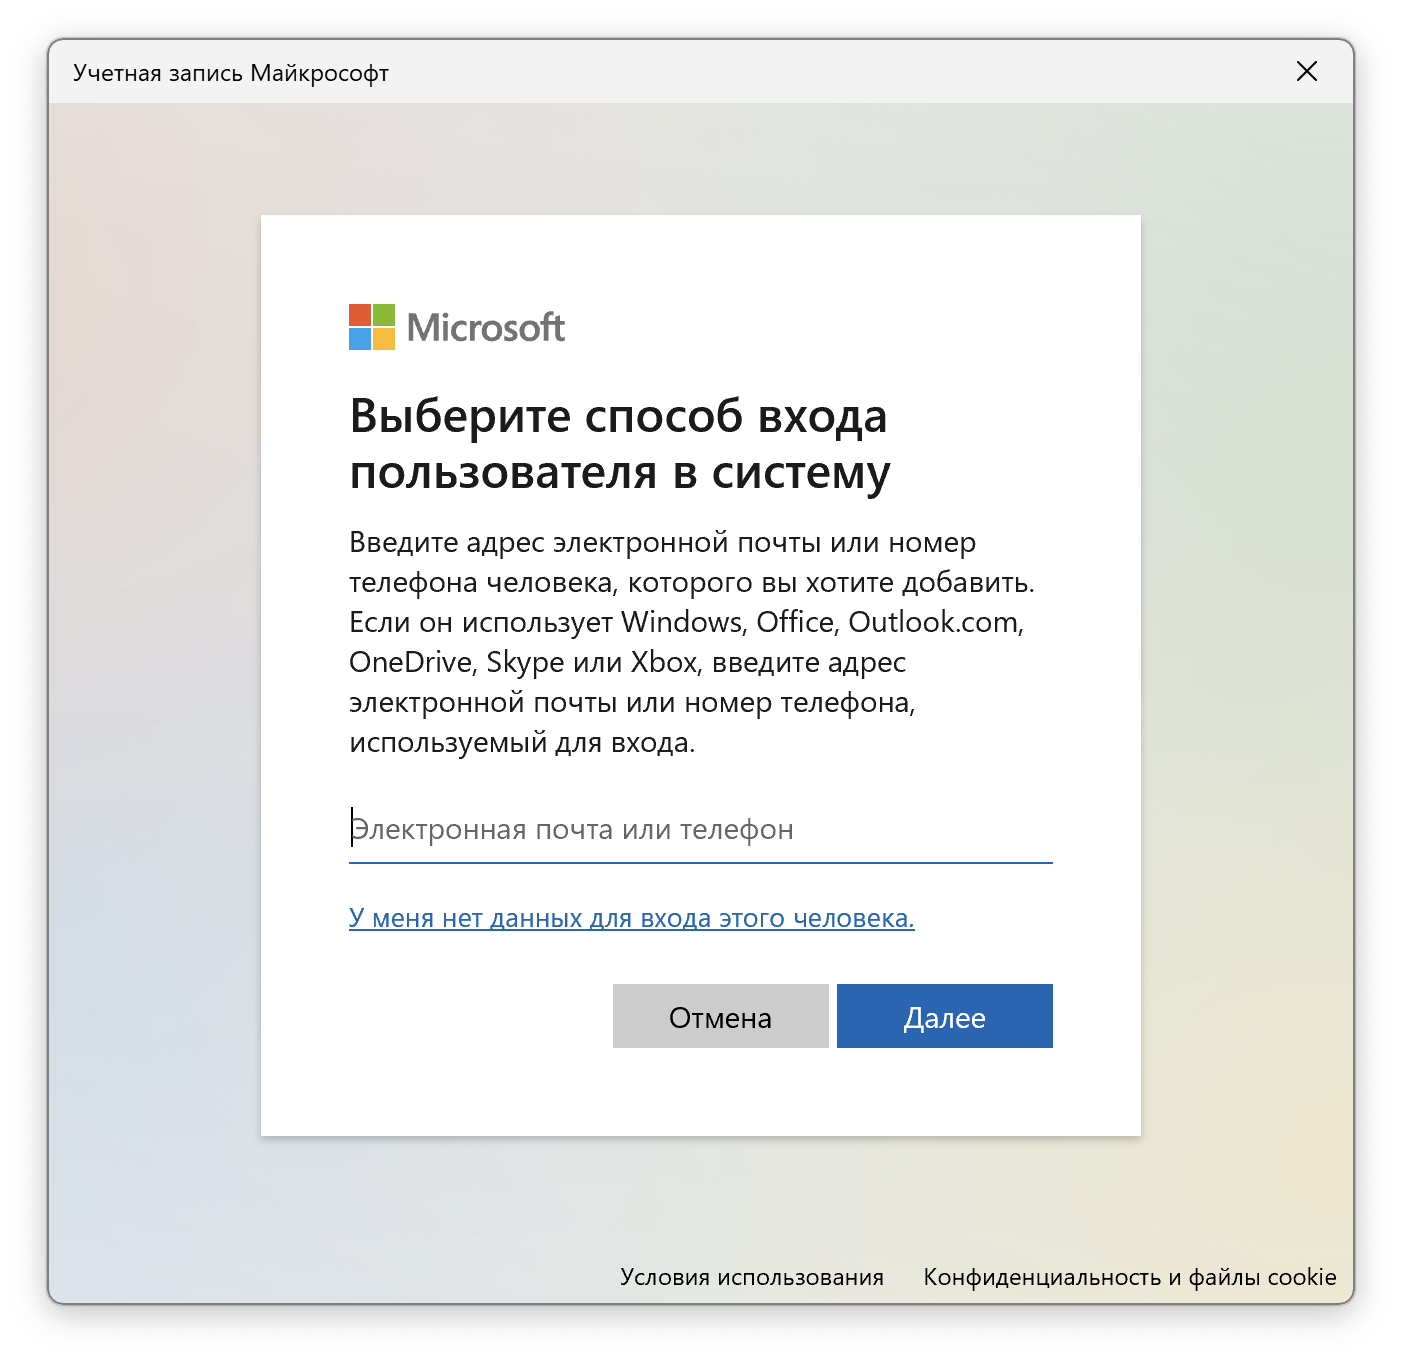
\includegraphics[width=0.8\textwidth]{../images/add_user.png}
              \caption{Добавление пользователя}
          \end{figure}
          }
    \item {Выберем: «Добавить пользователя без учетной записи Майкрософт»
          \begin{figure}[H]
              \centering
              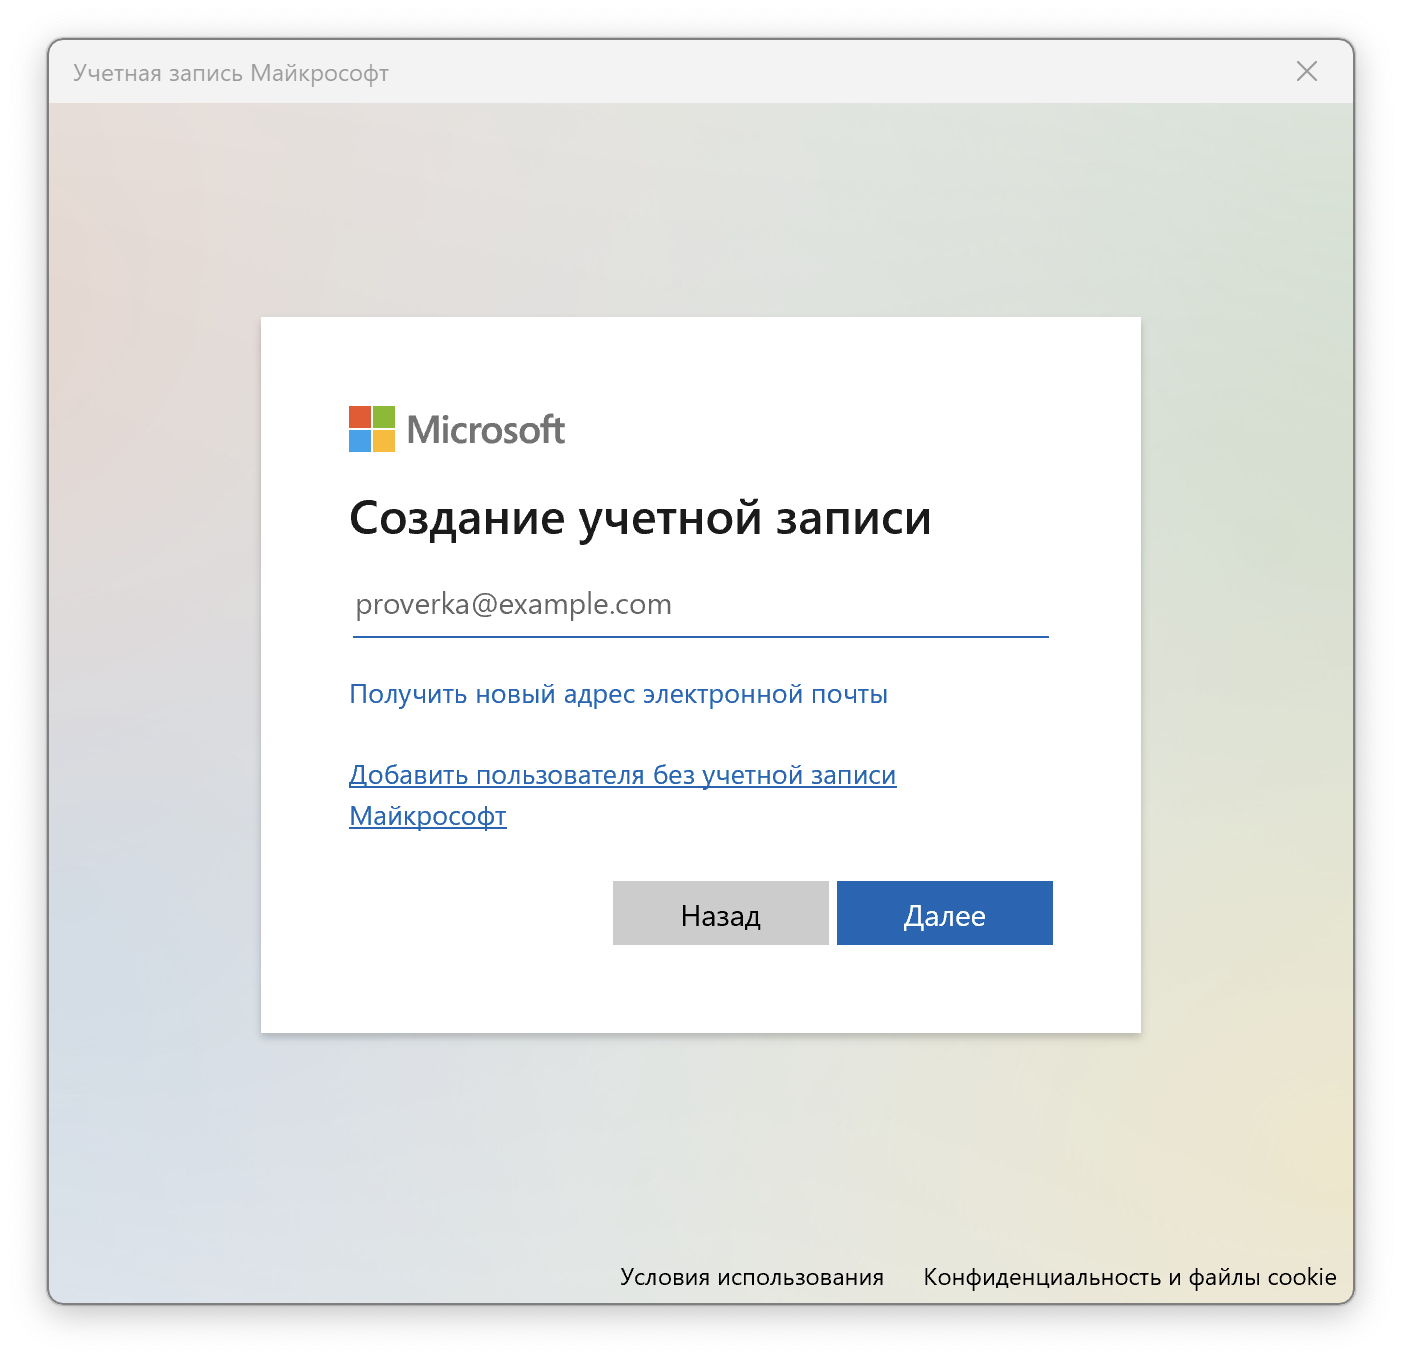
\includegraphics[width=0.8\textwidth]{../images/create_account.png}
              \caption{Создание учетной записи}
          \end{figure}
          }
    \item {Вводим имя пользователя, пароль и контрольные вопросы.
          \begin{figure}[H]
              \centering
              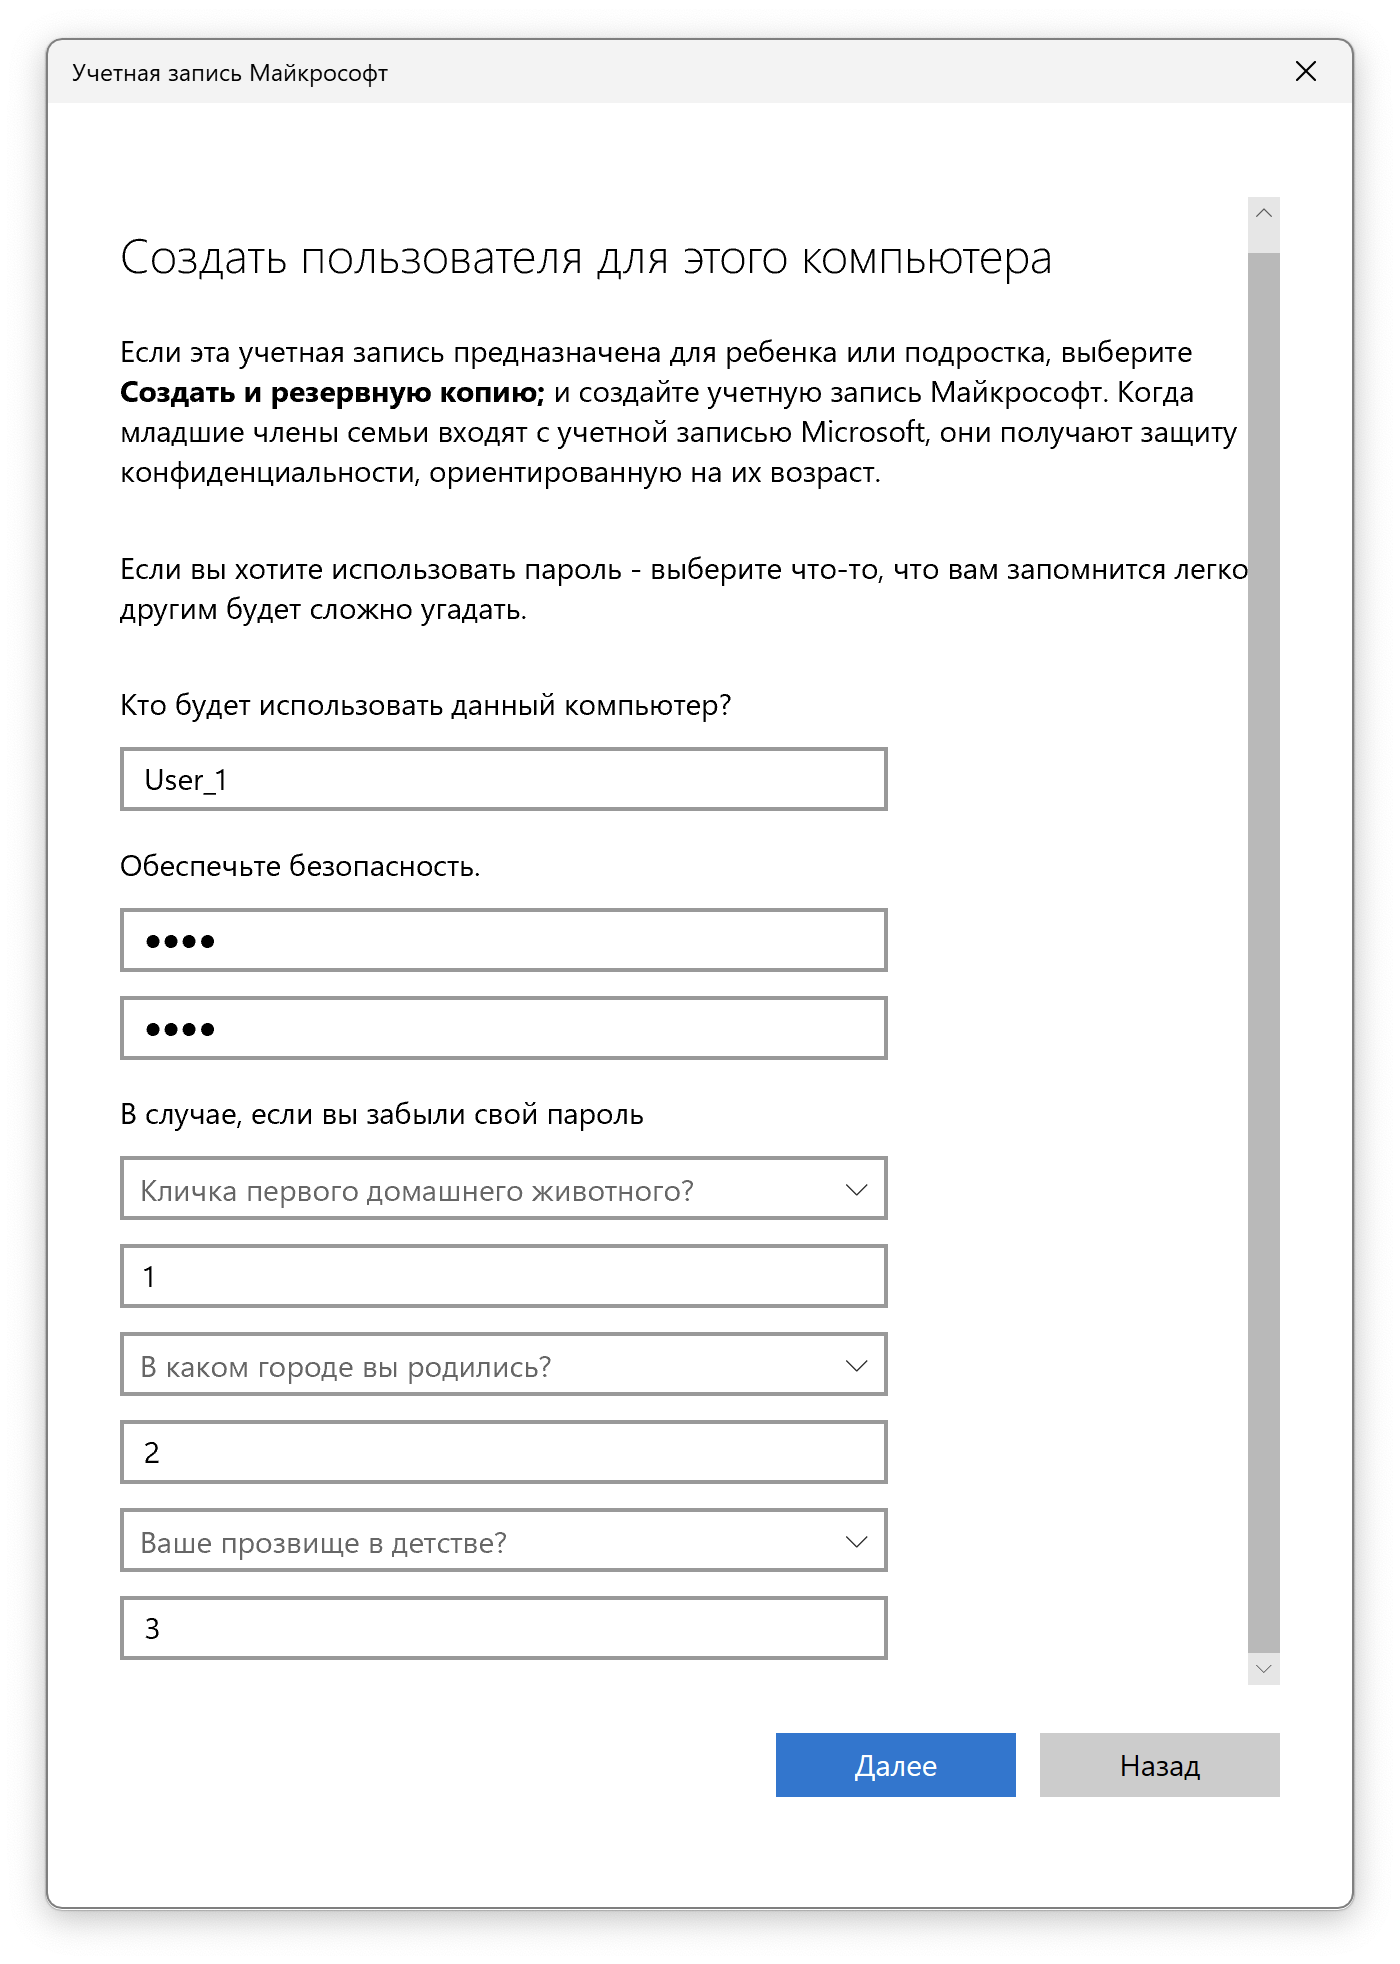
\includegraphics[width=0.8\textwidth]{../images/create_user.png}
              \caption{Создание пользователя}
          \end{figure}
          }
    \item {Пользователь создан.
          \begin{figure}[H]
              \centering
              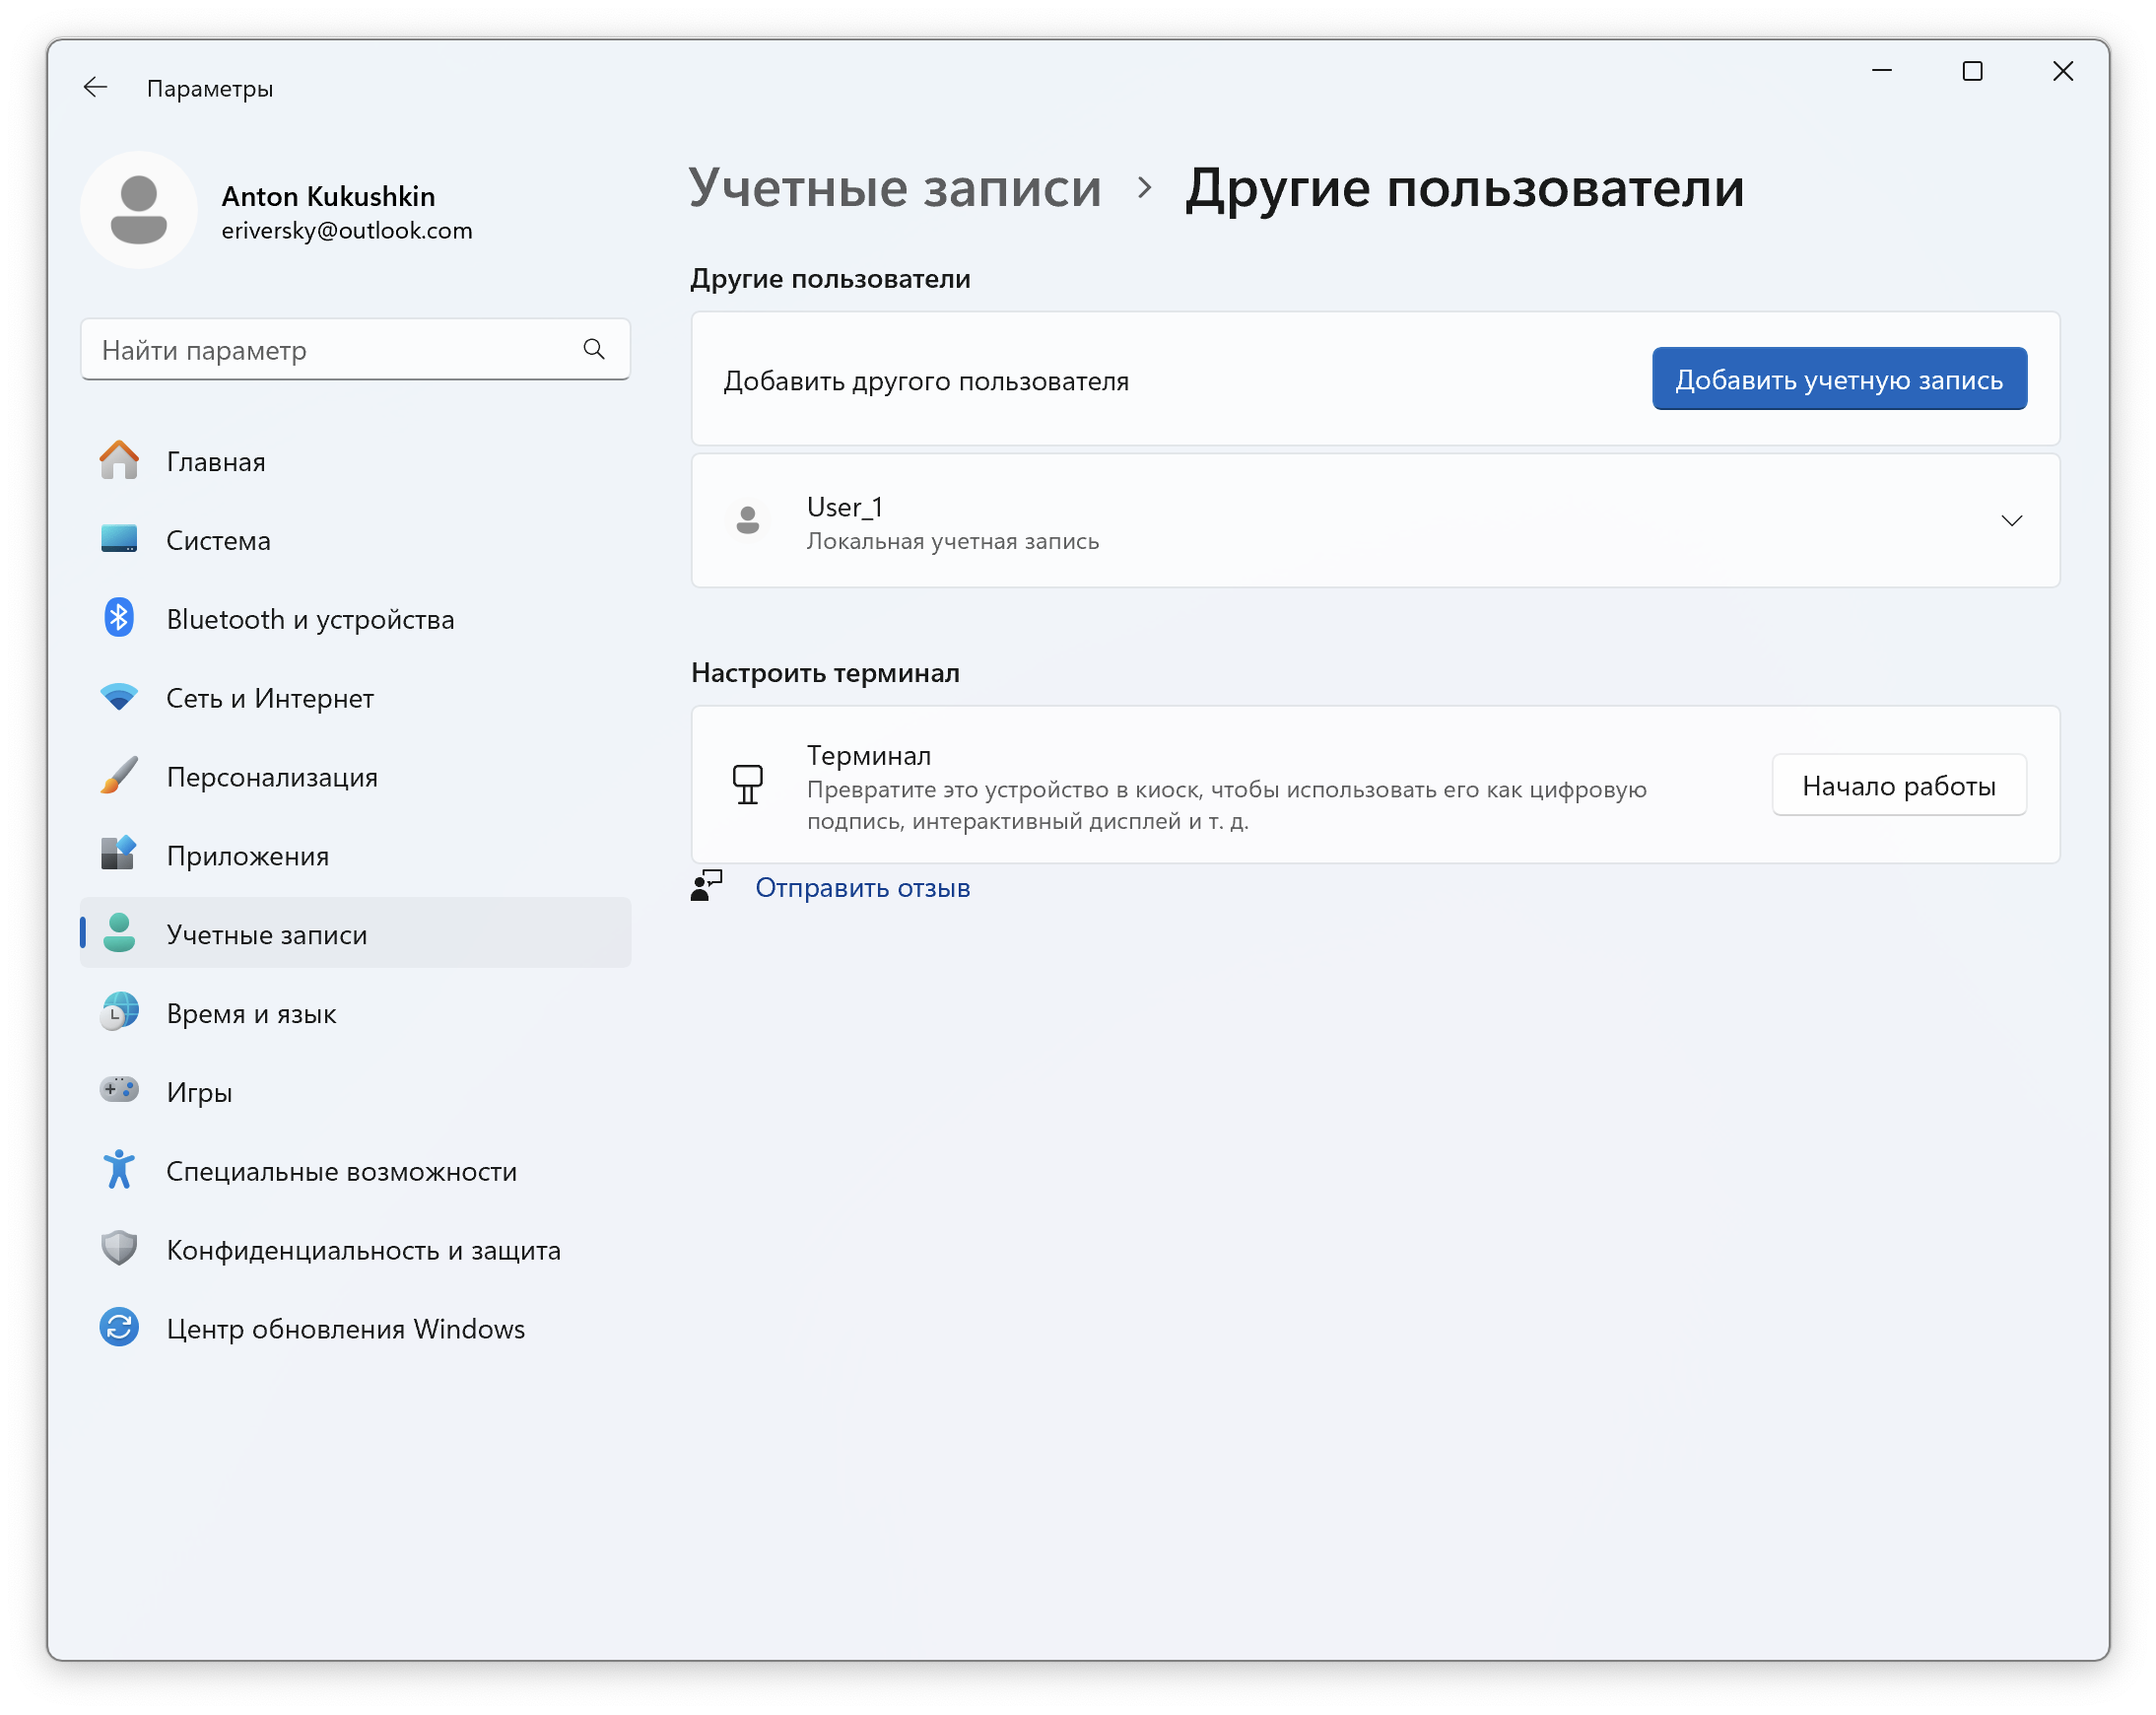
\includegraphics[width=0.8\textwidth]{../images/user_created.png}
              \caption{Пользователь создан}
          \end{figure}
          }
\end{enumerate}


\nsubsection{Вариант 2. Создание нового пользователя в Панели управления}
\begin{enumerate}
    \item {Переходим в Панель управления > Изменение типа учетной записи > Управление учетными записями > Добавить нового пользователя в окне "Параметры компьютера".
          \begin{figure}[H]
              \centering
              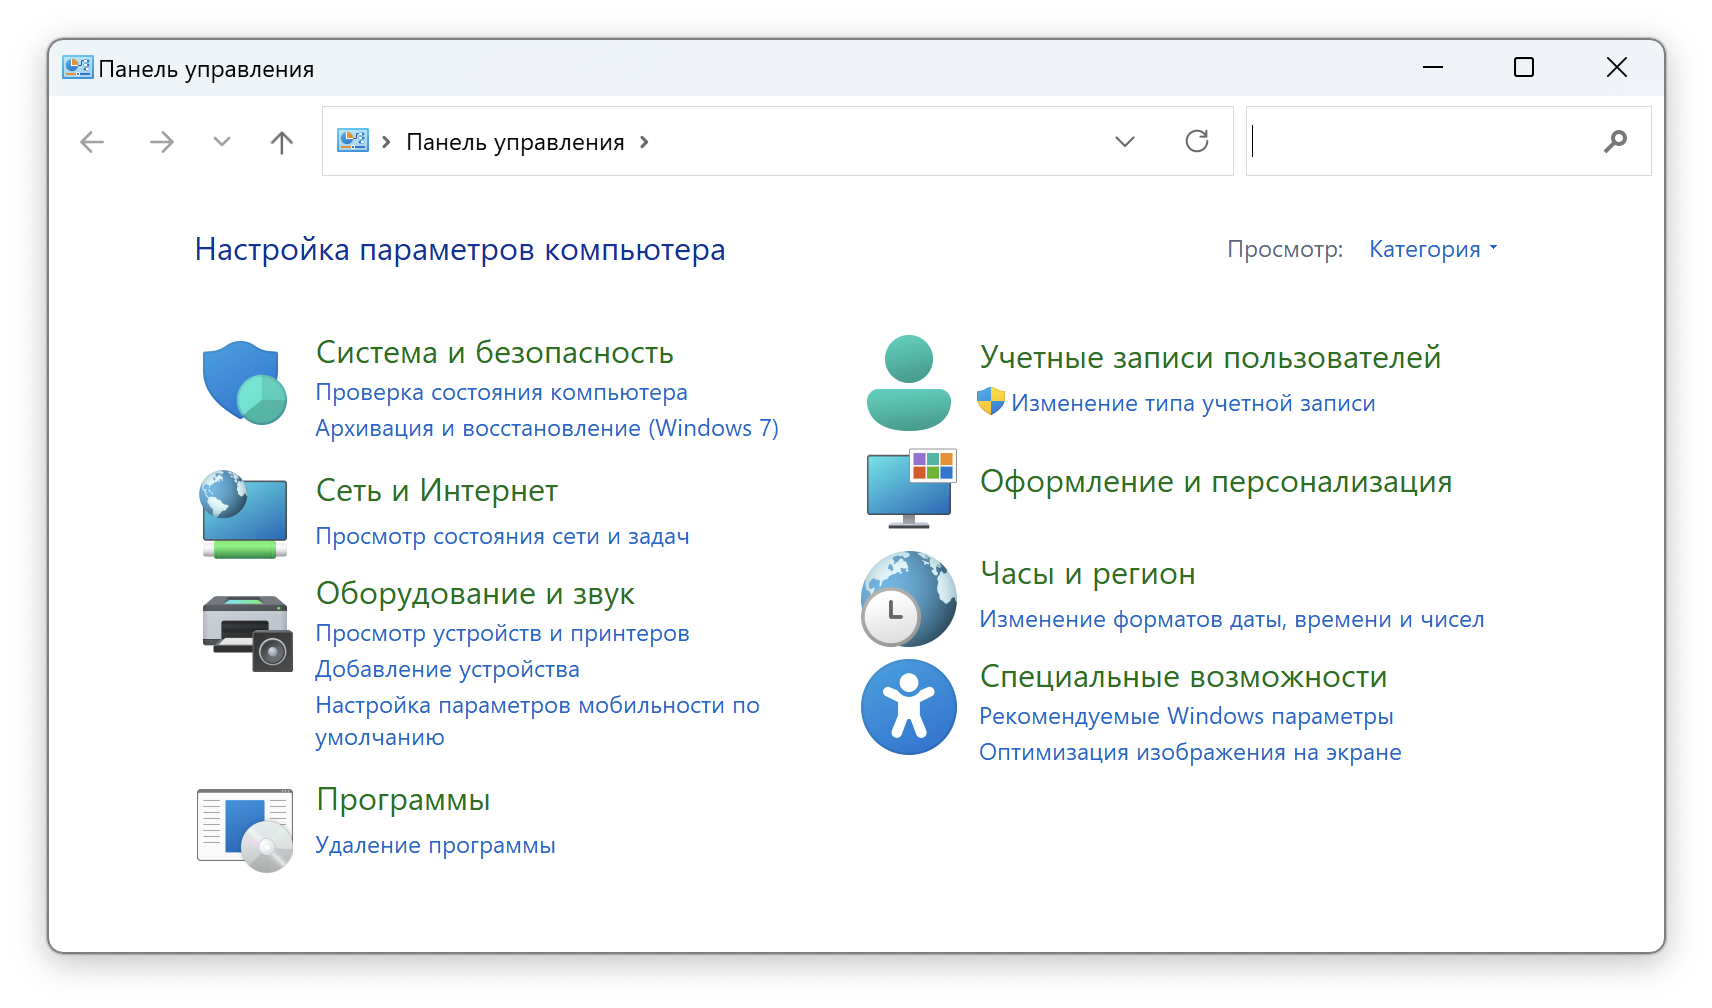
\includegraphics[width=0.8\textwidth]{../images/control_panel.png}
              \caption{Панель управления}
          \end{figure}
          \begin{figure}[H]
              \centering
              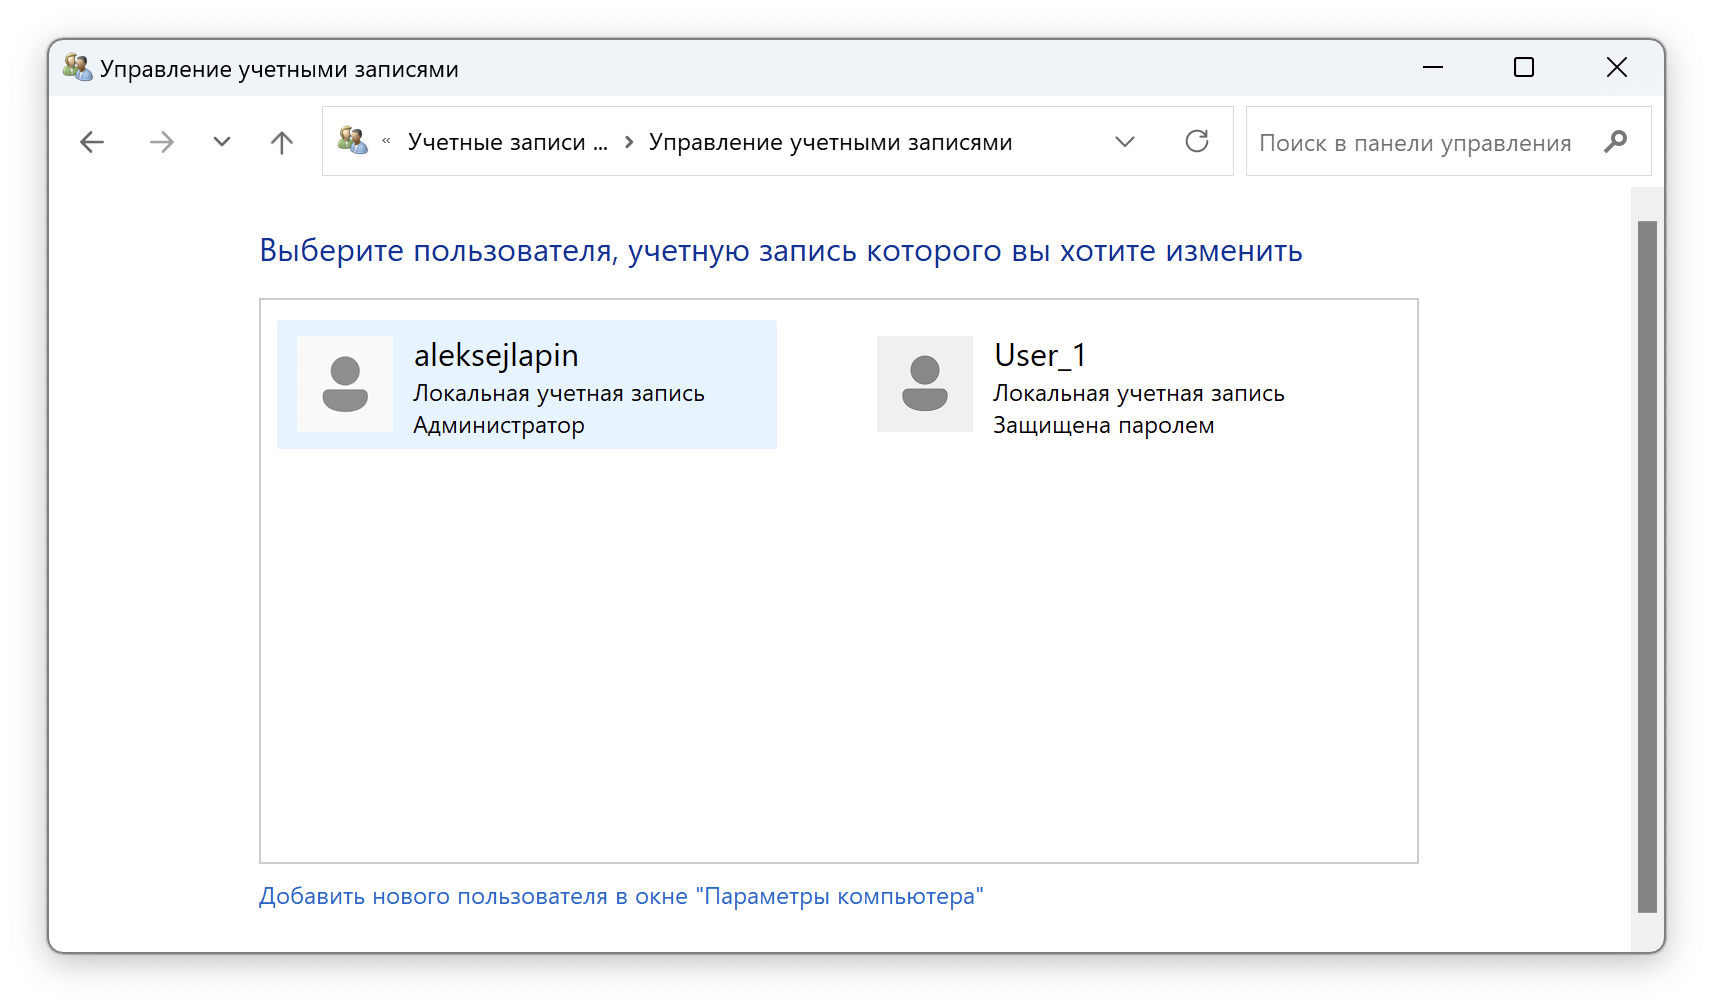
\includegraphics[width=0.8\textwidth]{../images/account_management.png}
              \caption{Управление учетными записями}
          \end{figure}
          }
    \item {Дальше все действия аналогичны варианту 1.
          \begin{figure}[H]
              \centering
              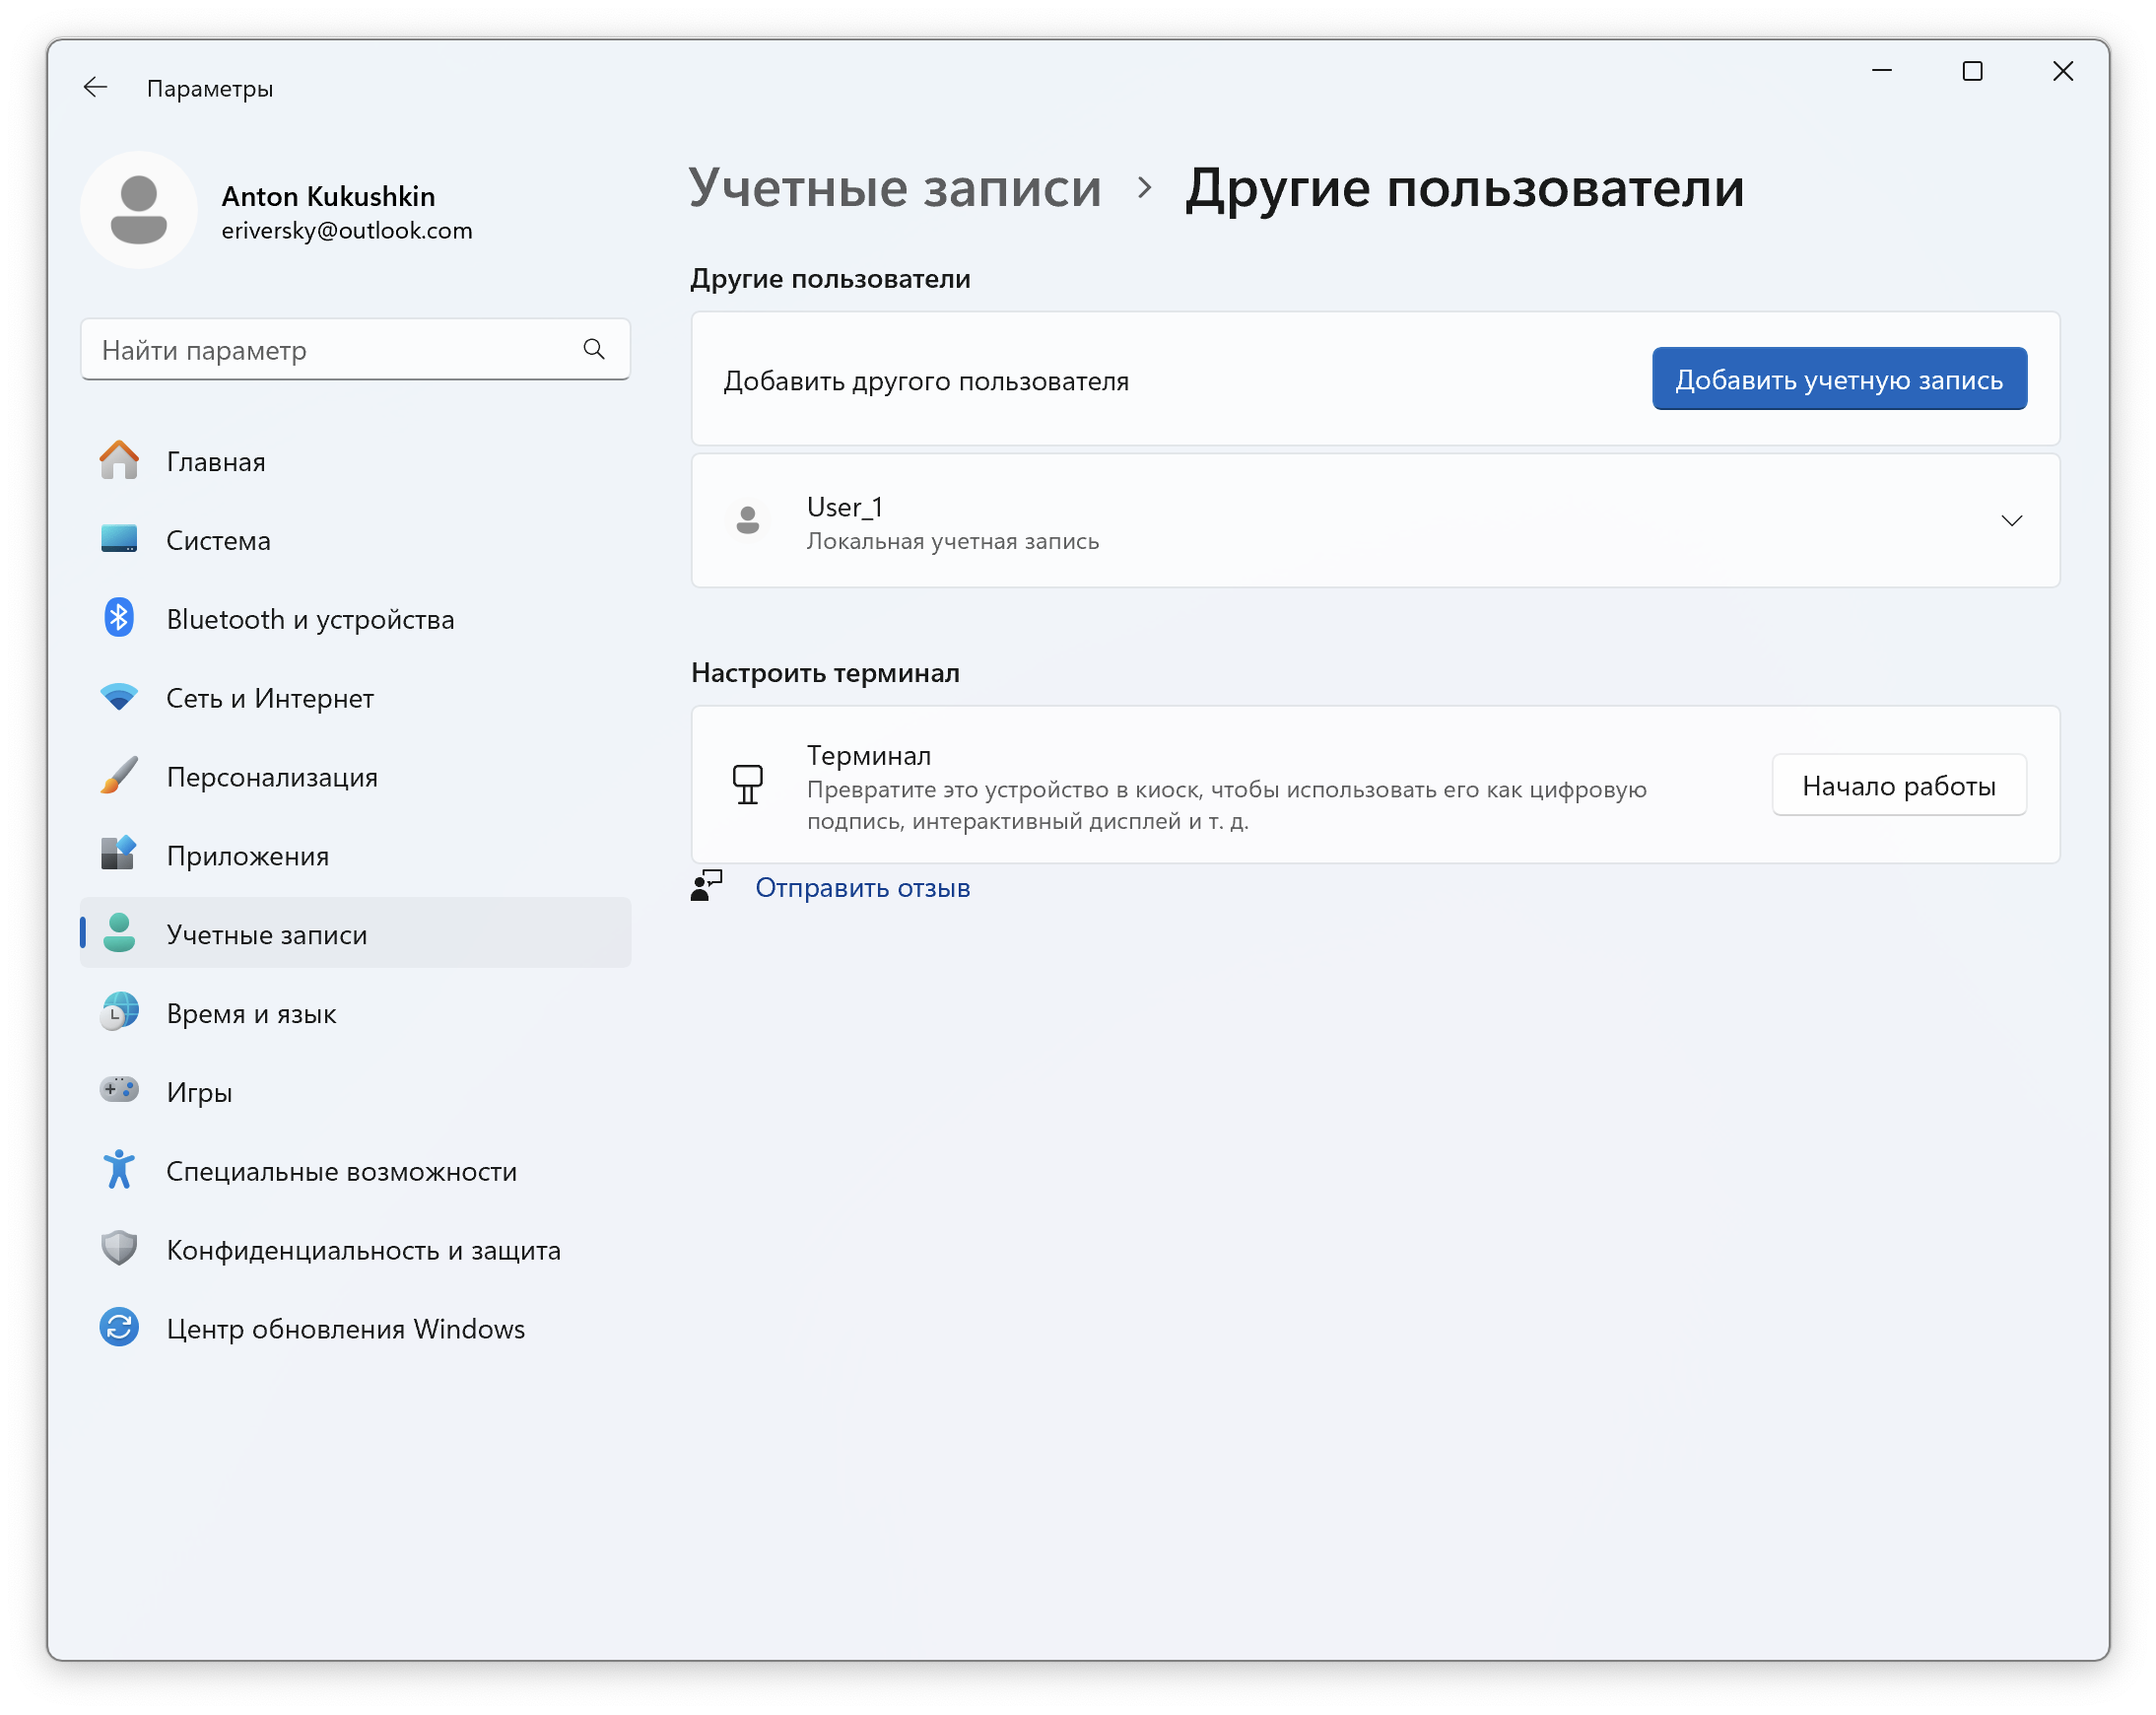
\includegraphics[width=0.8\textwidth]{../images/user_created.png}
              \caption{Другие пользователи}
          \end{figure}
          }
\end{enumerate}

\nsubsection{Вариант 3. Создание пользователя в окне управления учетными записями пользователей}
\begin{enumerate}
    \item { Нажмите Ctrl + R, введите \texttt{control userpasswords2} и нажмите Enter.
          \begin{figure}[H]
              \centering
              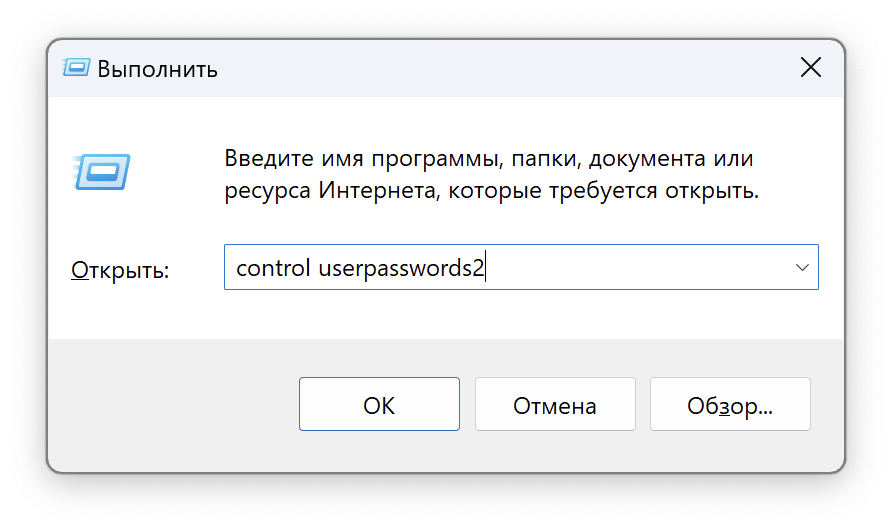
\includegraphics[width=0.8\textwidth]{../images/execute_command.png}
              \caption{Выполнение команды}
          \end{figure}
          \begin{figure}[H]
              \centering
              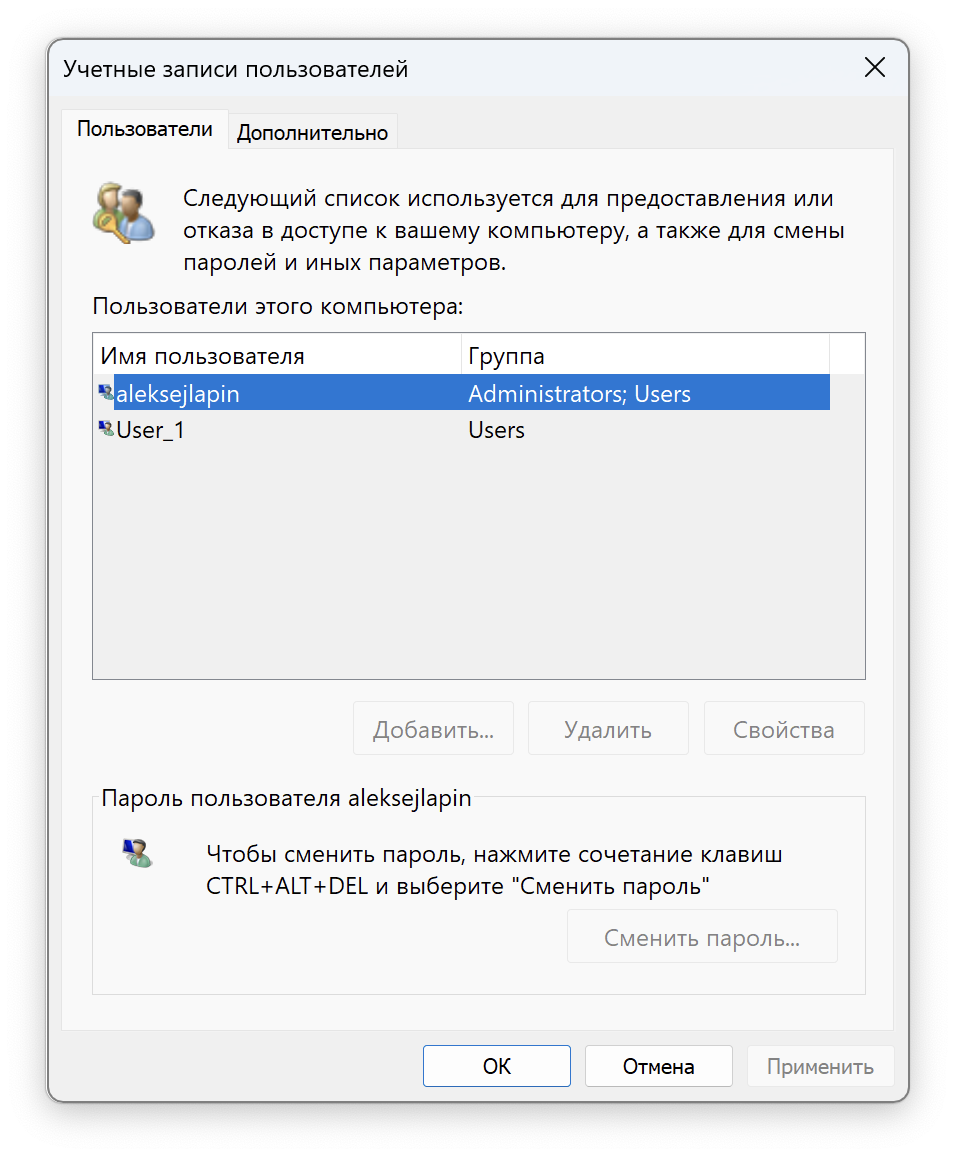
\includegraphics[width=0.8\textwidth]{../images/control_userpasswords2.png}
              \caption{Управление учетными записями пользователей}
          \end{figure}
          }
    \item {Переходим в раздел «Дополнительно».
          \begin{figure}[H]
              \centering
              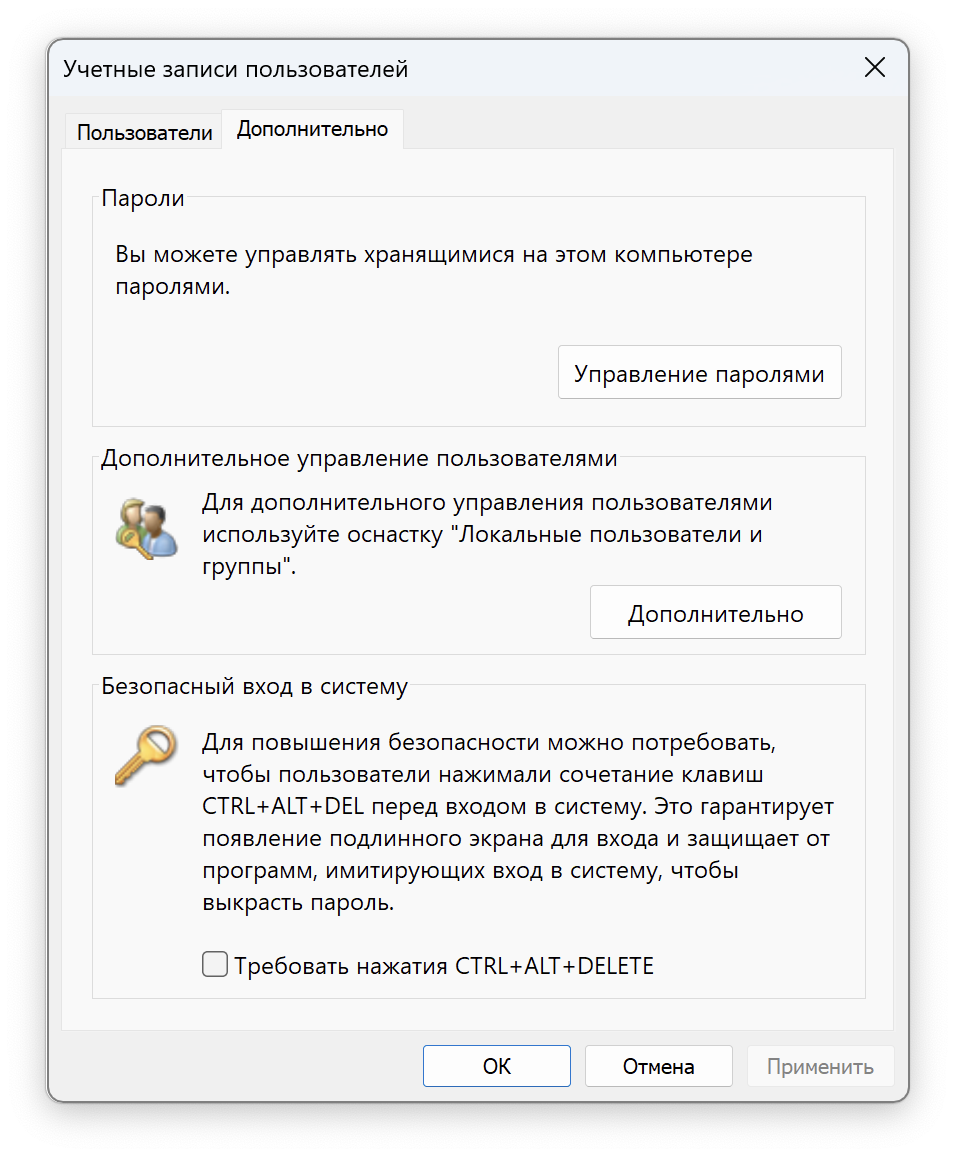
\includegraphics[width=0.8\textwidth]{../images/control_userpasswords2_extra.png}
              \caption{Управление учетными записями пользователей (дополнительные параметры)}
          \end{figure}
          }
    \item {Открывается окно управления локальными пользователями и группами.
          \begin{figure}[H]
              \centering
              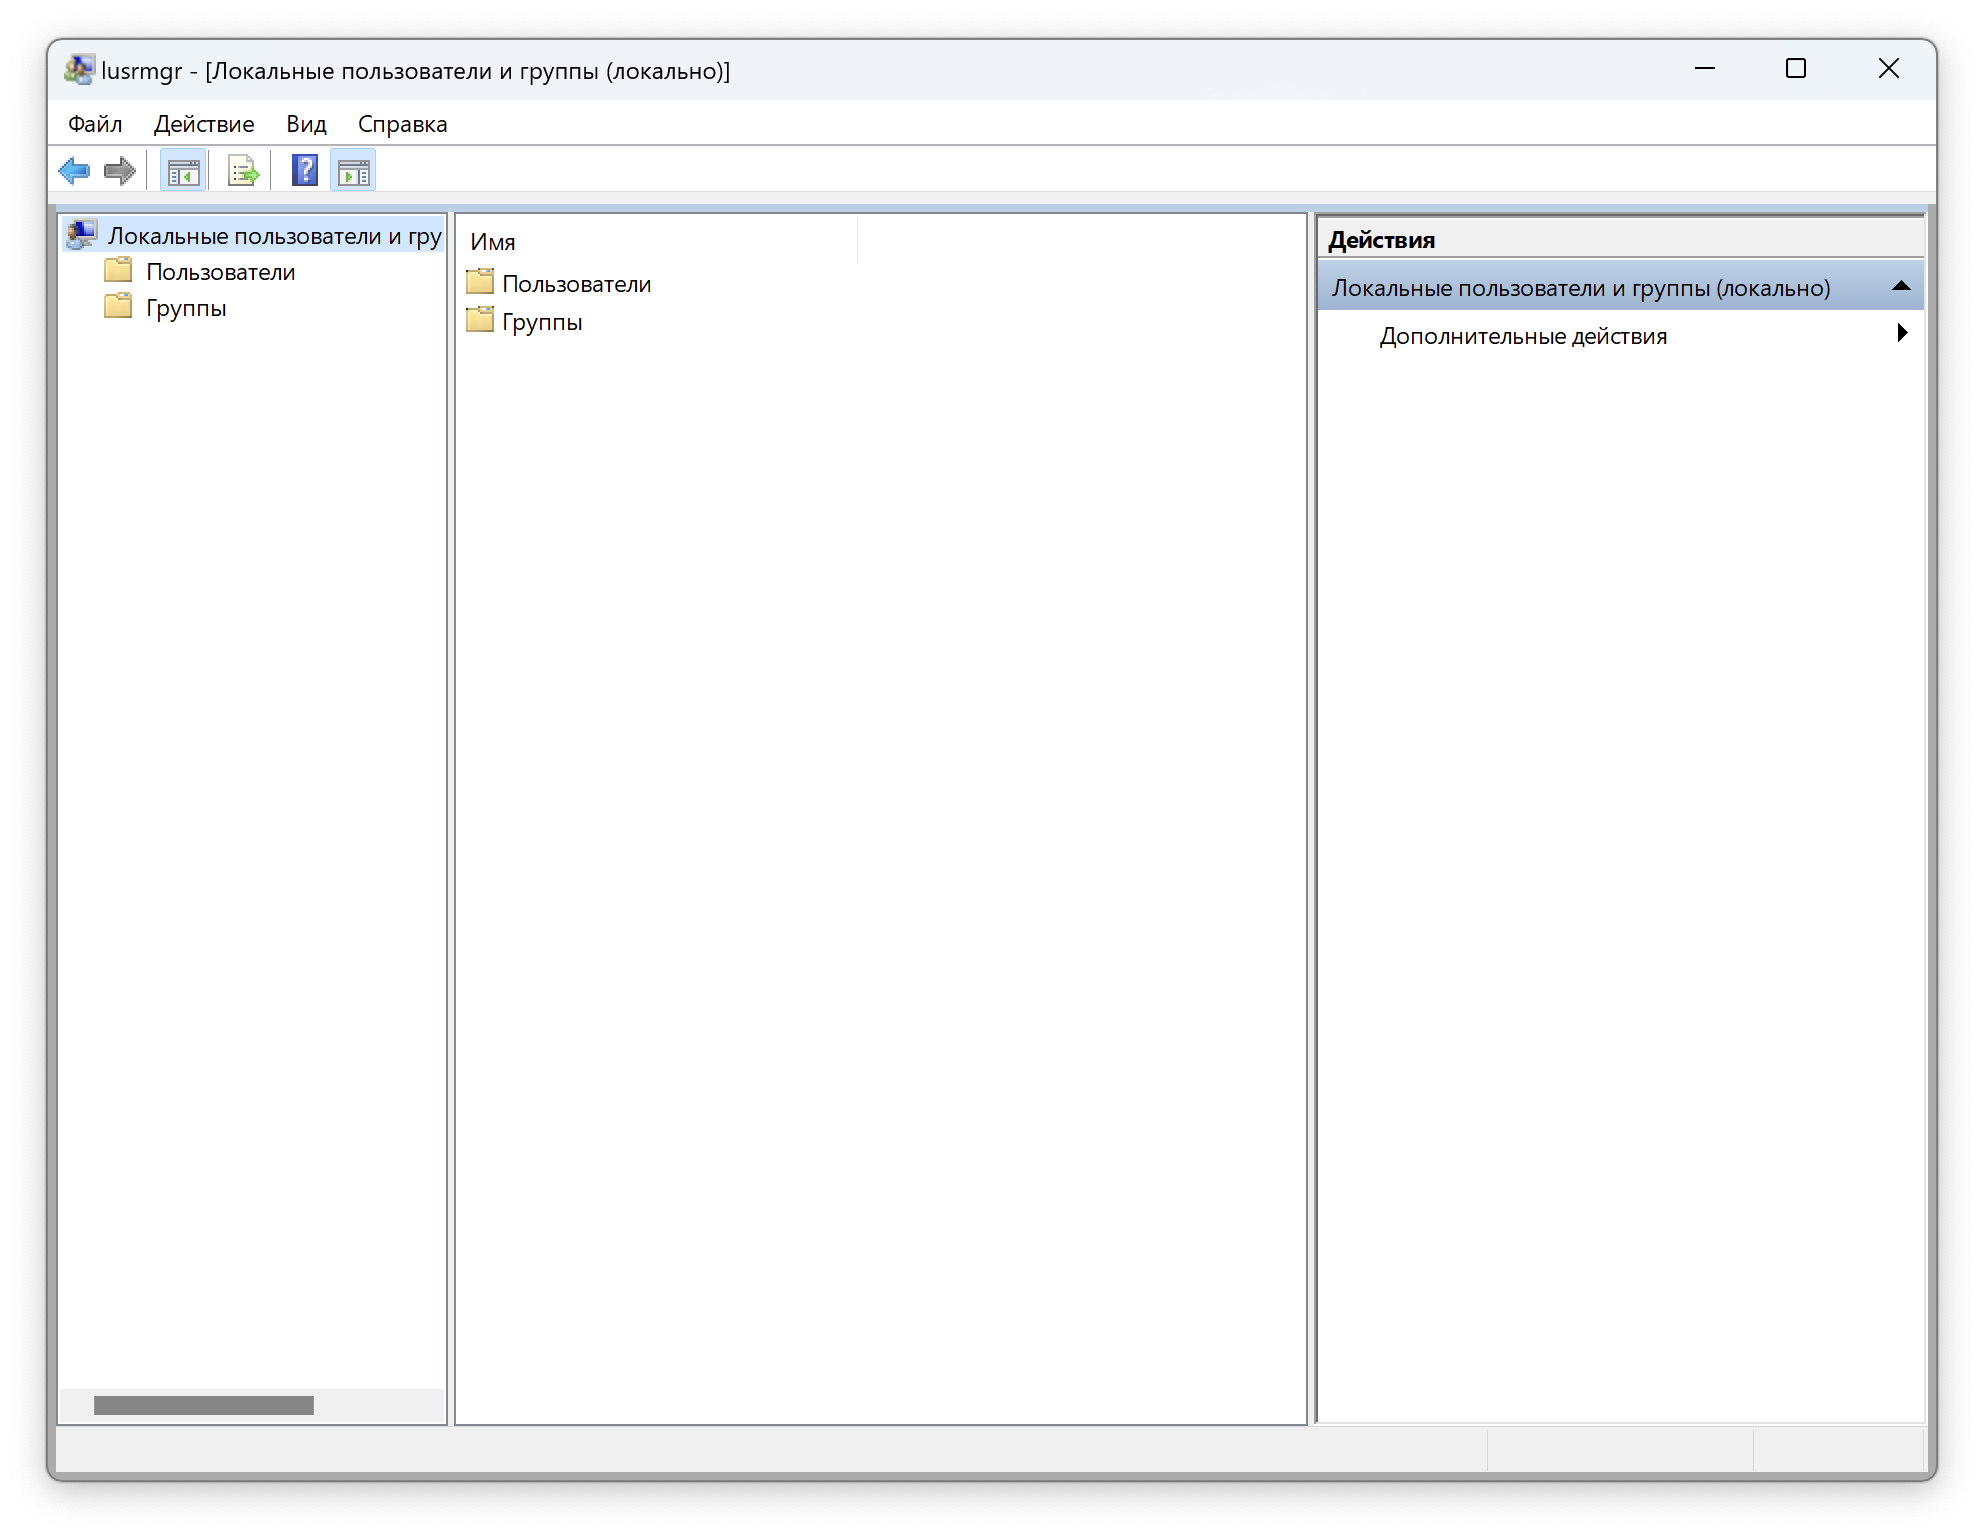
\includegraphics[width=0.8\textwidth]{../images/lusrmgr.png}
              \caption{Управление локальными пользователями и группами}
          \end{figure}
          }
    \item {Нажимаем правой кнопкой мыши на «Пользователи» и выбираем «Новый пользователь...»
          \begin{figure}[H]
              \centering
              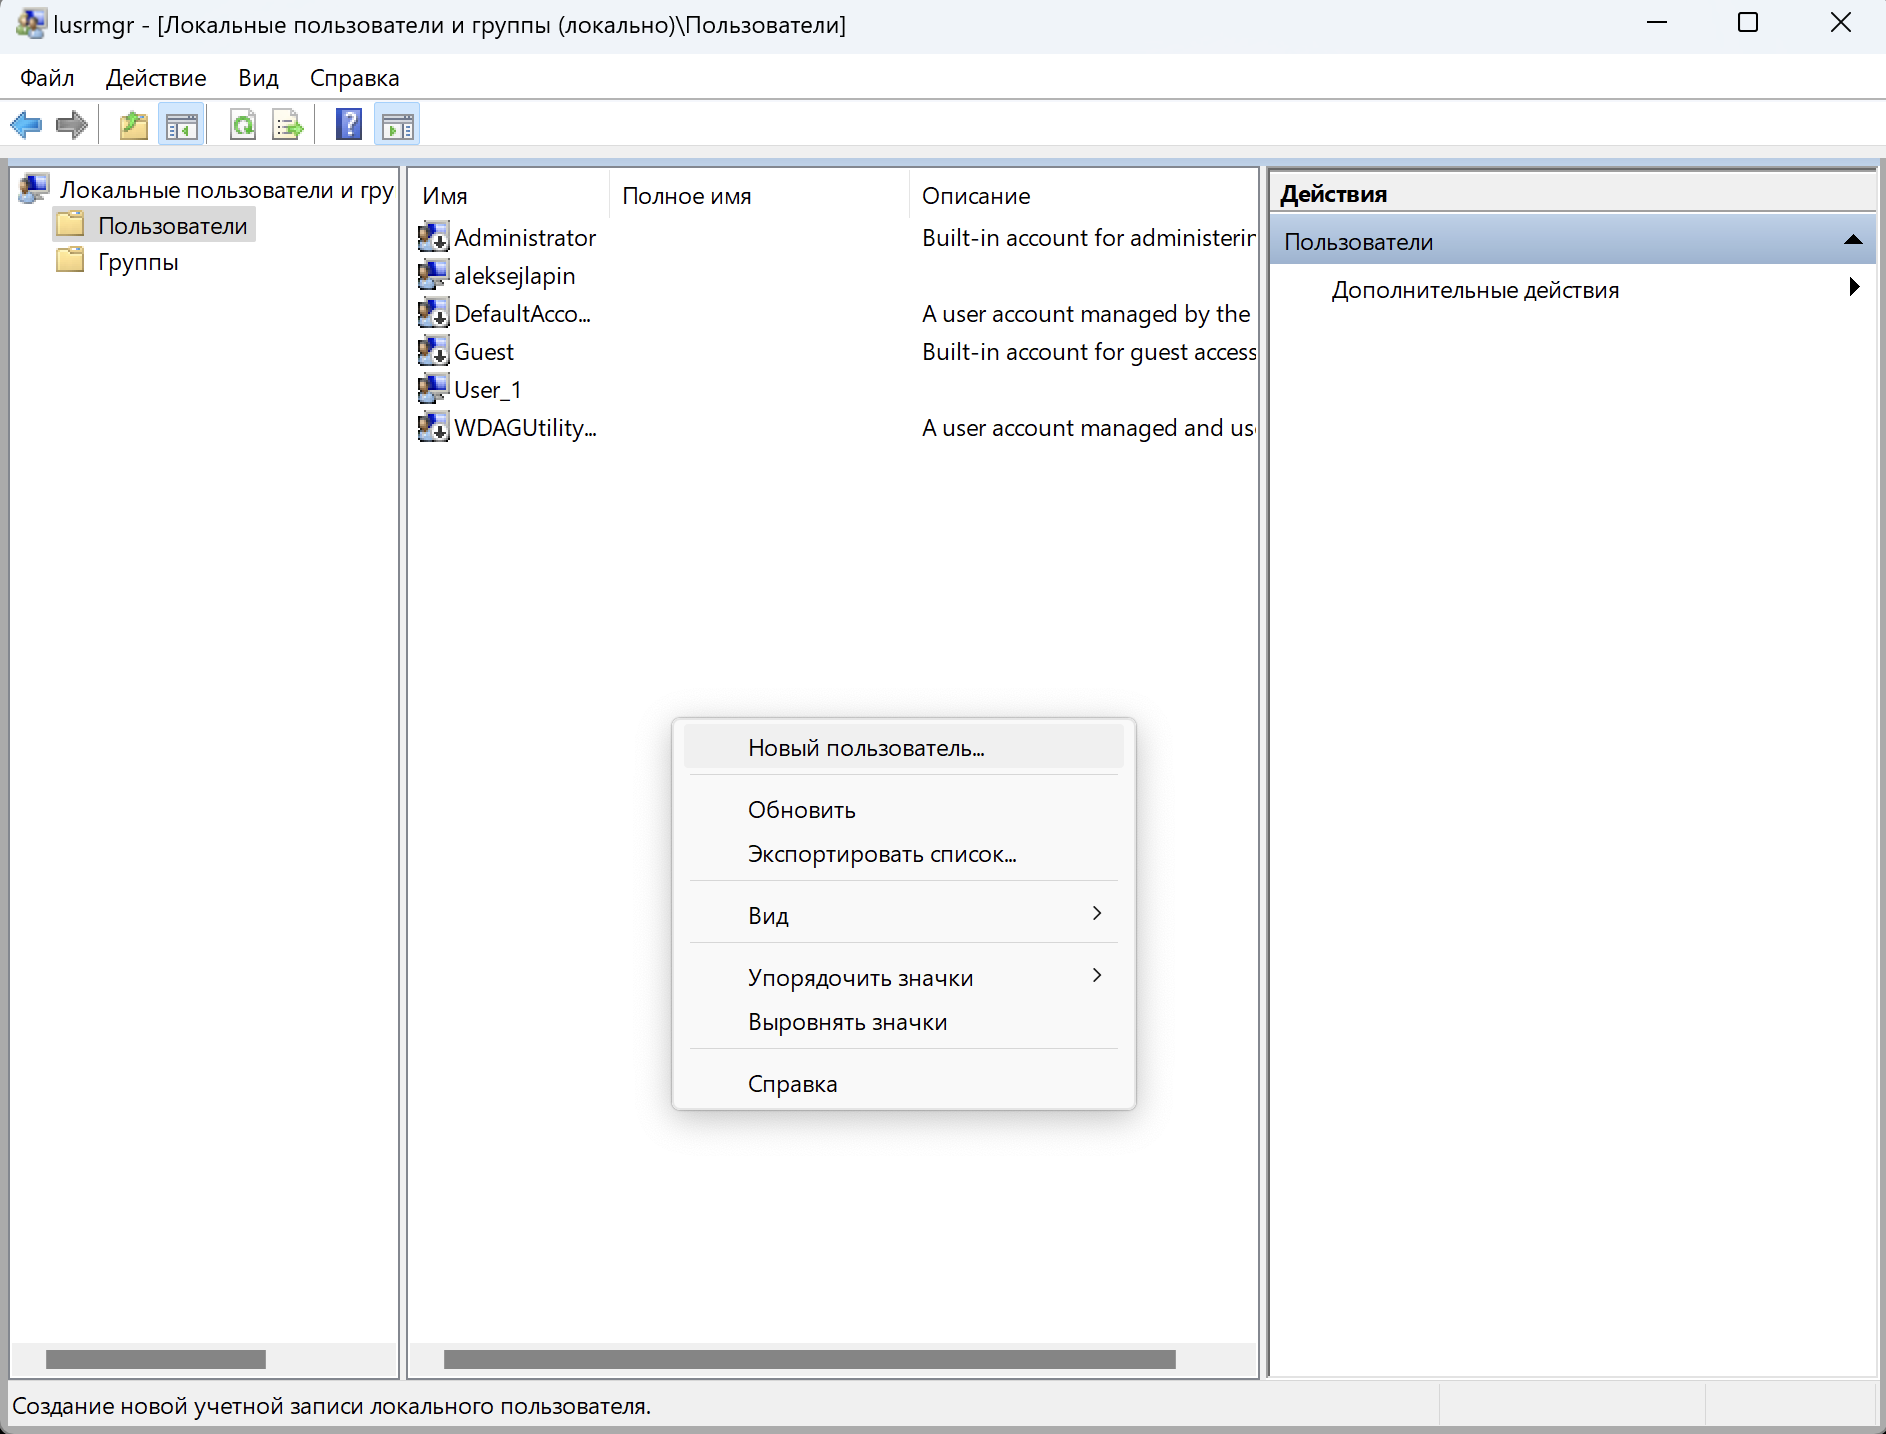
\includegraphics[width=0.8\textwidth]{../images/lusrmgr_users.png}
              \caption{Управление локальными пользователями и группами (пользователи)}
          \end{figure}
          }
    \item {Вводим имя пользователя, полное имя и пароль.
          \begin{figure}[H]
              \centering
              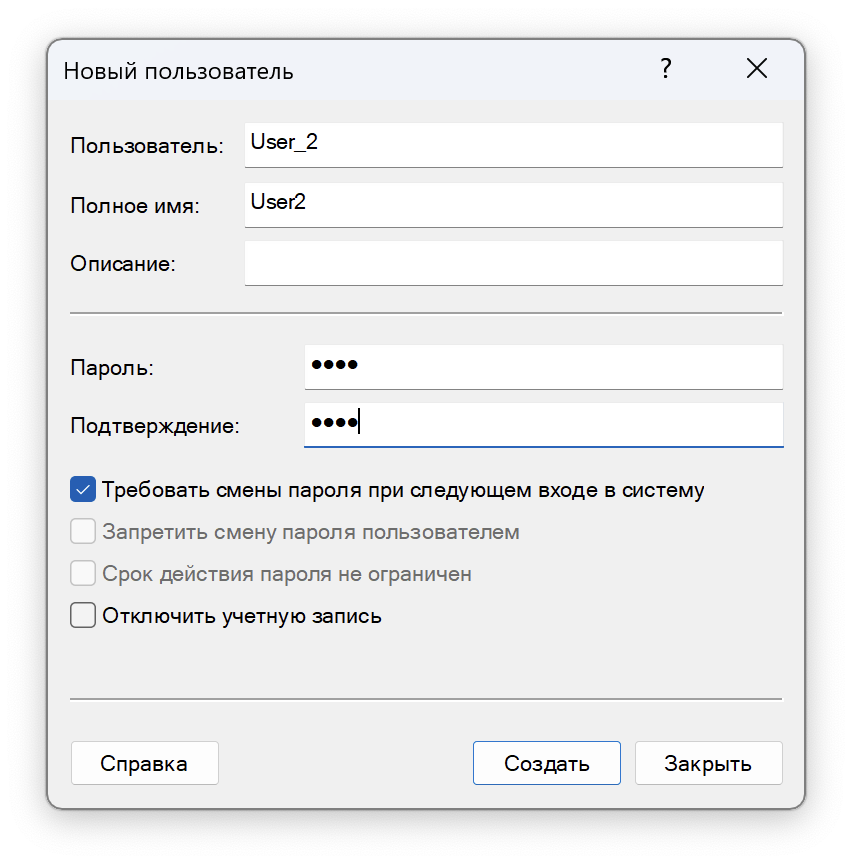
\includegraphics[width=0.8\textwidth]{../images/lusrmgr_create_user.png}
              \caption{Создание нового пользователя}
          \end{figure}
          }
    \item {Новый пользователь создан.
          \begin{figure}[H]
              \centering
              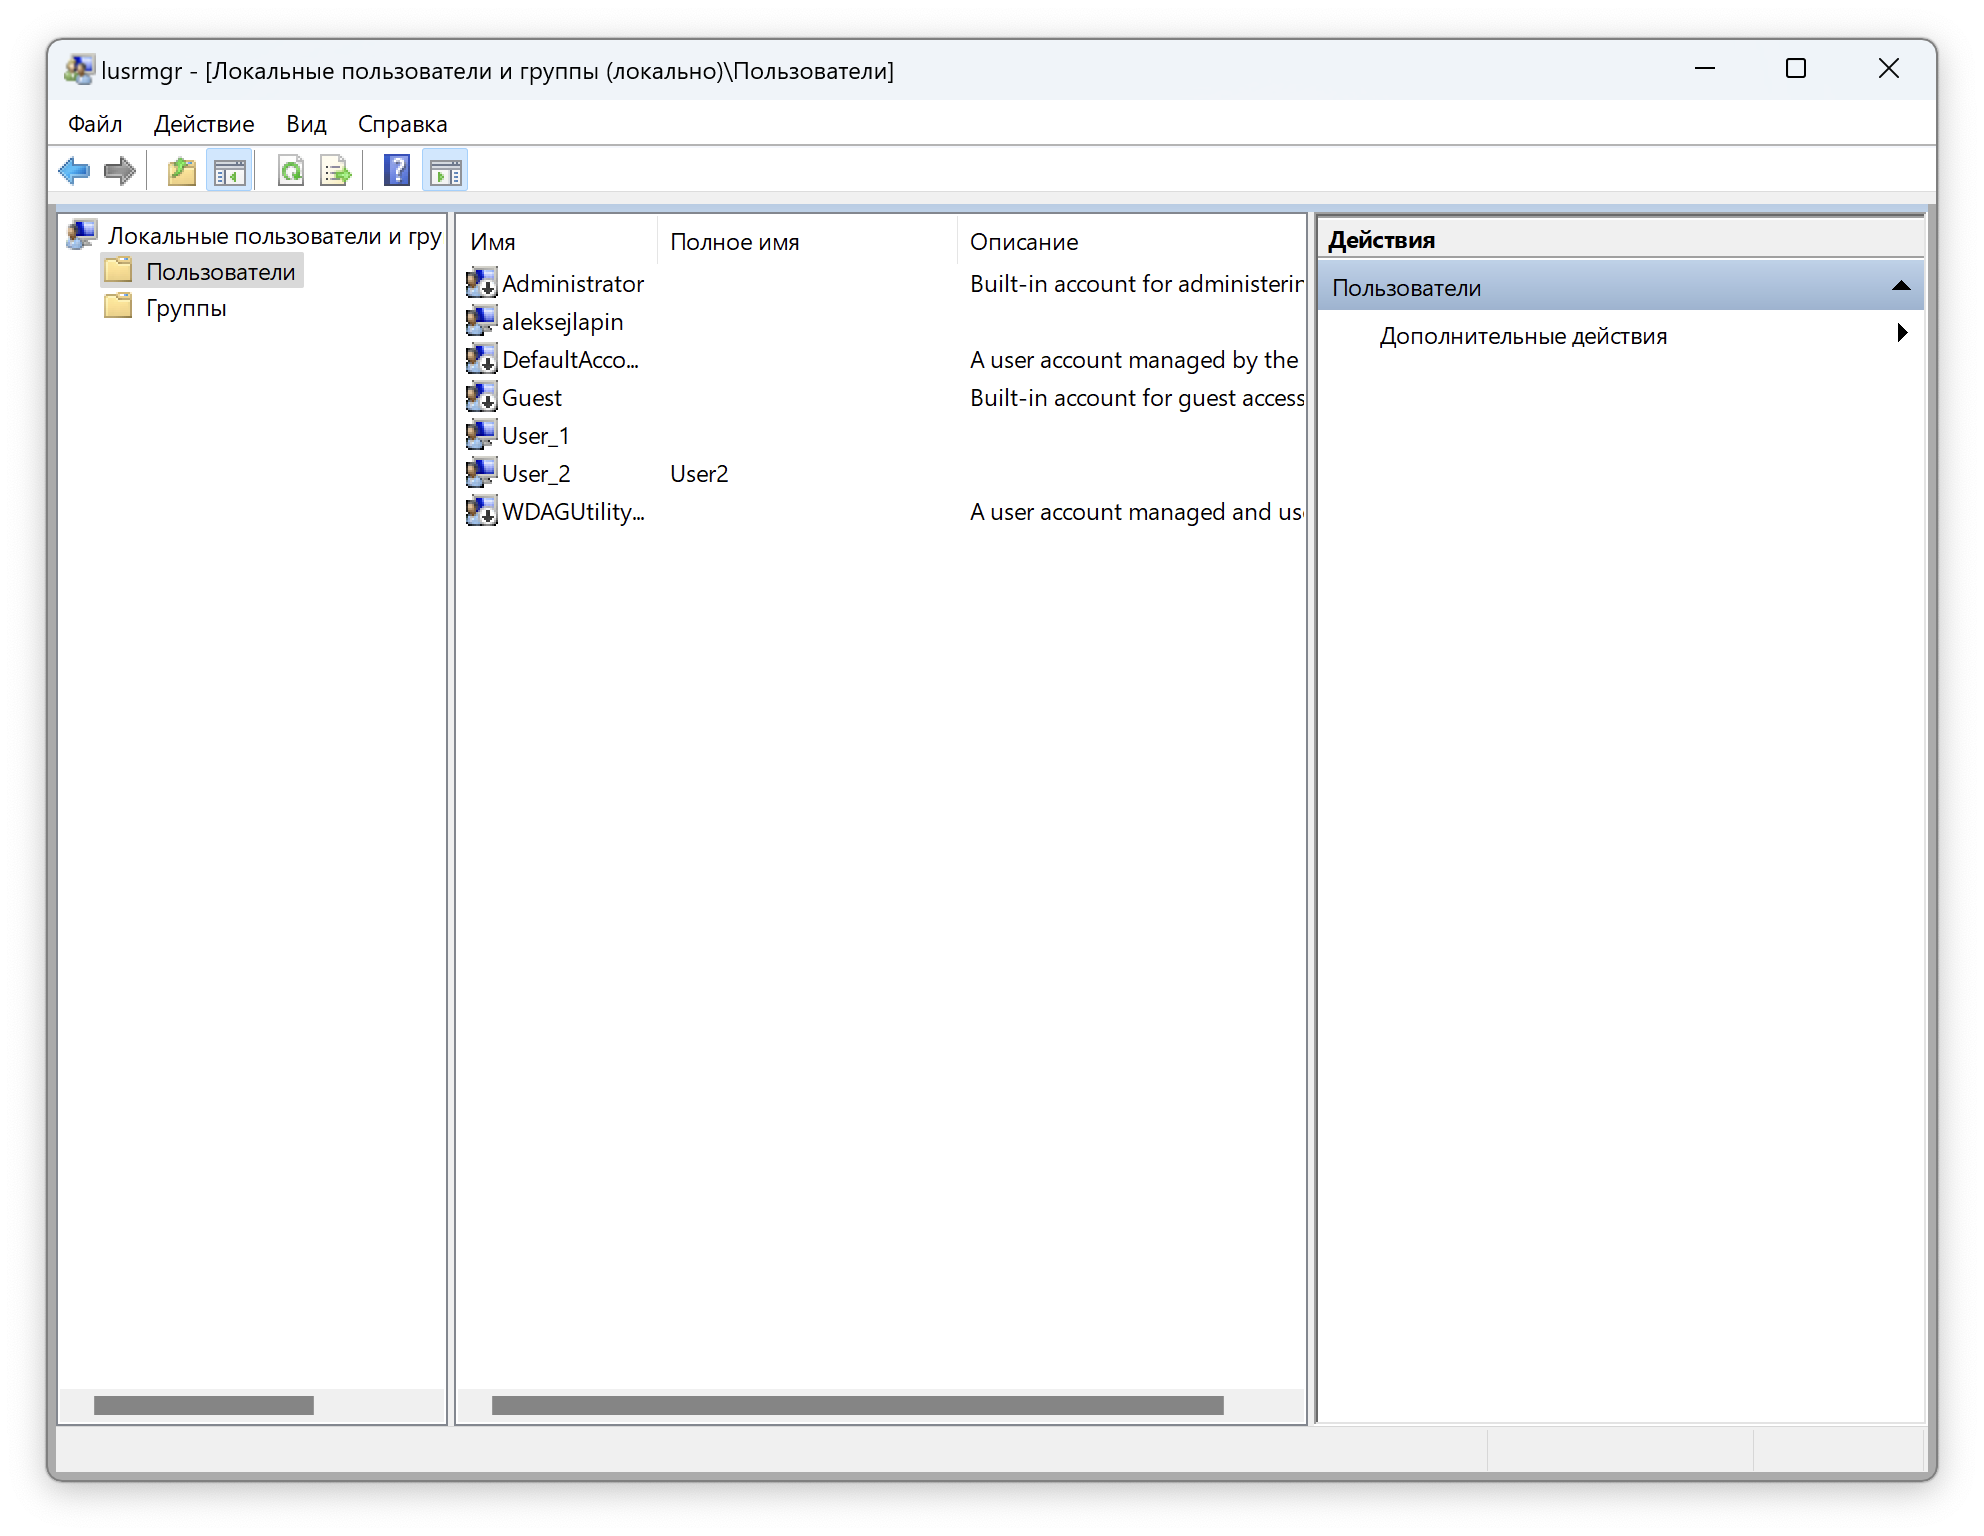
\includegraphics[width=0.8\textwidth]{../images/lusrmgr_new_user.png}
              \caption{Новый пользователь}
          \end{figure}
          }
\end{enumerate}

\nsubsection{Вариант 4. Создание пользователя с помощью командной строки}
\begin{enumerate}
    \item {Откроем командную строку от имени администратора.}
    \item {Введем команду \texttt{net user <имя пользователя> <пароль> /add}}
    \item {Если пользователь создан, то появится сообщение: \texttt{Команда выполнена успешно.}
          \begin{figure}[H]
              \centering
              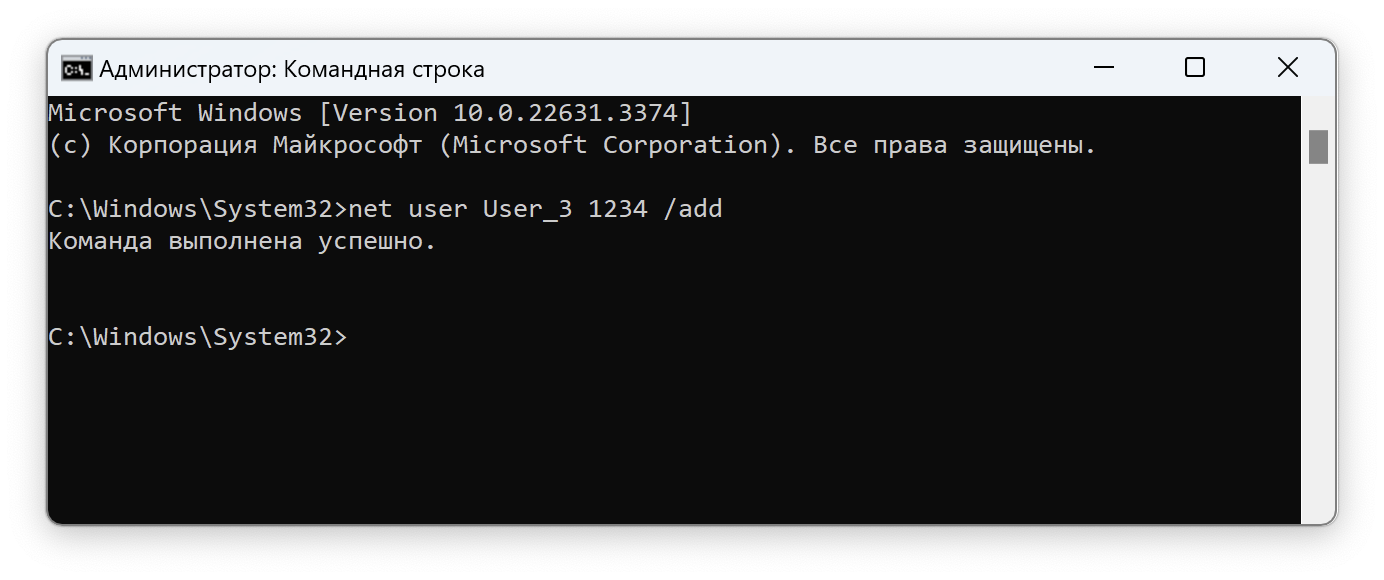
\includegraphics[width=0.8\textwidth]{../images/cmd_create_user.png}
              \caption{Создание пользователя с помощью командной строки}
          \end{figure}
          }
    \item \textbf{Описание команды NET USER}
          \begin{enumerate}
              \item Команда \texttt{NET USER} предназначена для добавления, редактирования или просмотра учетных записей пользователей на компьютерах. При выполнении команды в командной строке без параметров отображается список учетных записей пользователей Windows, присутствующих на компьютере.
              \item \textbf{Возможности команды Net User}
                    \begin{itemize}
                        \item Добавить учетную запись;
                        \item Добавить пароль учетной записи;
                        \item Изменить пароль учетной записи;
                        \item Отключить учетную запись;
                        \item Удалить учетную запись.
                    \end{itemize}
          \end{enumerate}
\end{enumerate}

\nsubsection{Вариант 5. Создание пользователя с помощью PowerShell}

\begin{enumerate}
    \item {Откроем PowerShell от имени администратора.}
    \item {Введем команду \texttt{New-LocalUser}}
    \item {Введем имя пользователя и пароль.}
    \item {Если пользователь создан, то появится сообщение: \texttt{True}}
    \item {Пользователь создан.
          \begin{figure}[H]
              \centering
              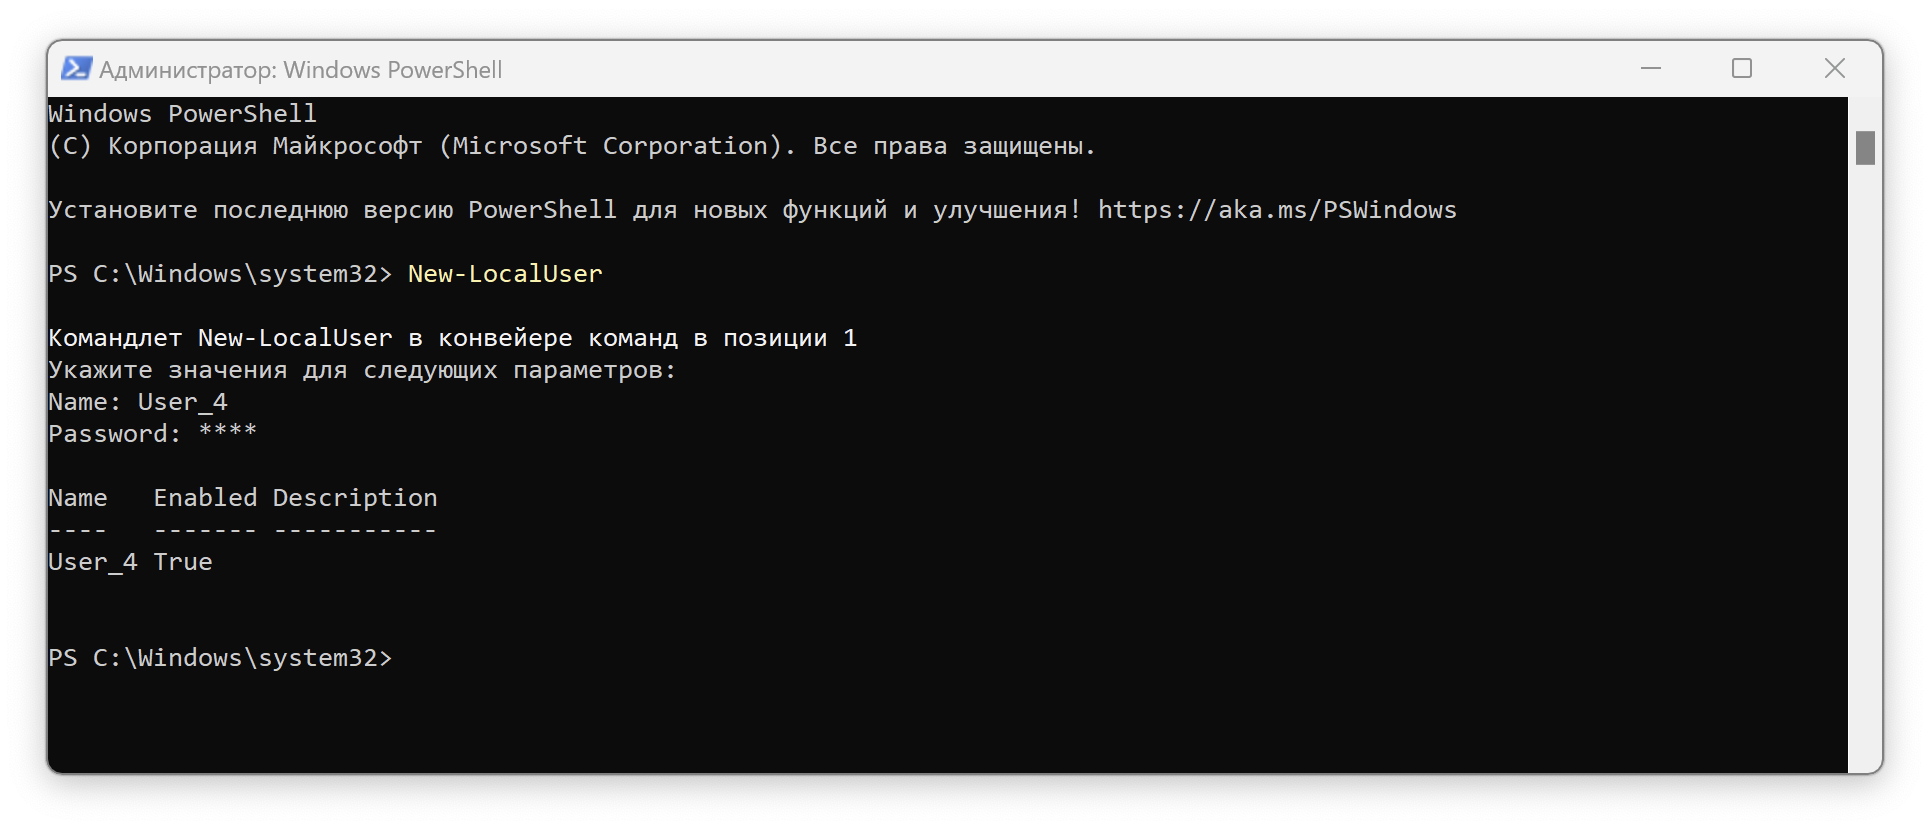
\includegraphics[width=0.8\textwidth]{../images/powershell_create_user.png}
              \caption{Создание пользователя с помощью PowerShell}
          \end{figure}}
\end{enumerate}

\nsubsection{Возможности пользователя по изменению конфигурации системы}
\begin{enumerate}
    \item {Пользователь может менять настройки региона и языка.
          \begin{figure}[H]
              \centering
              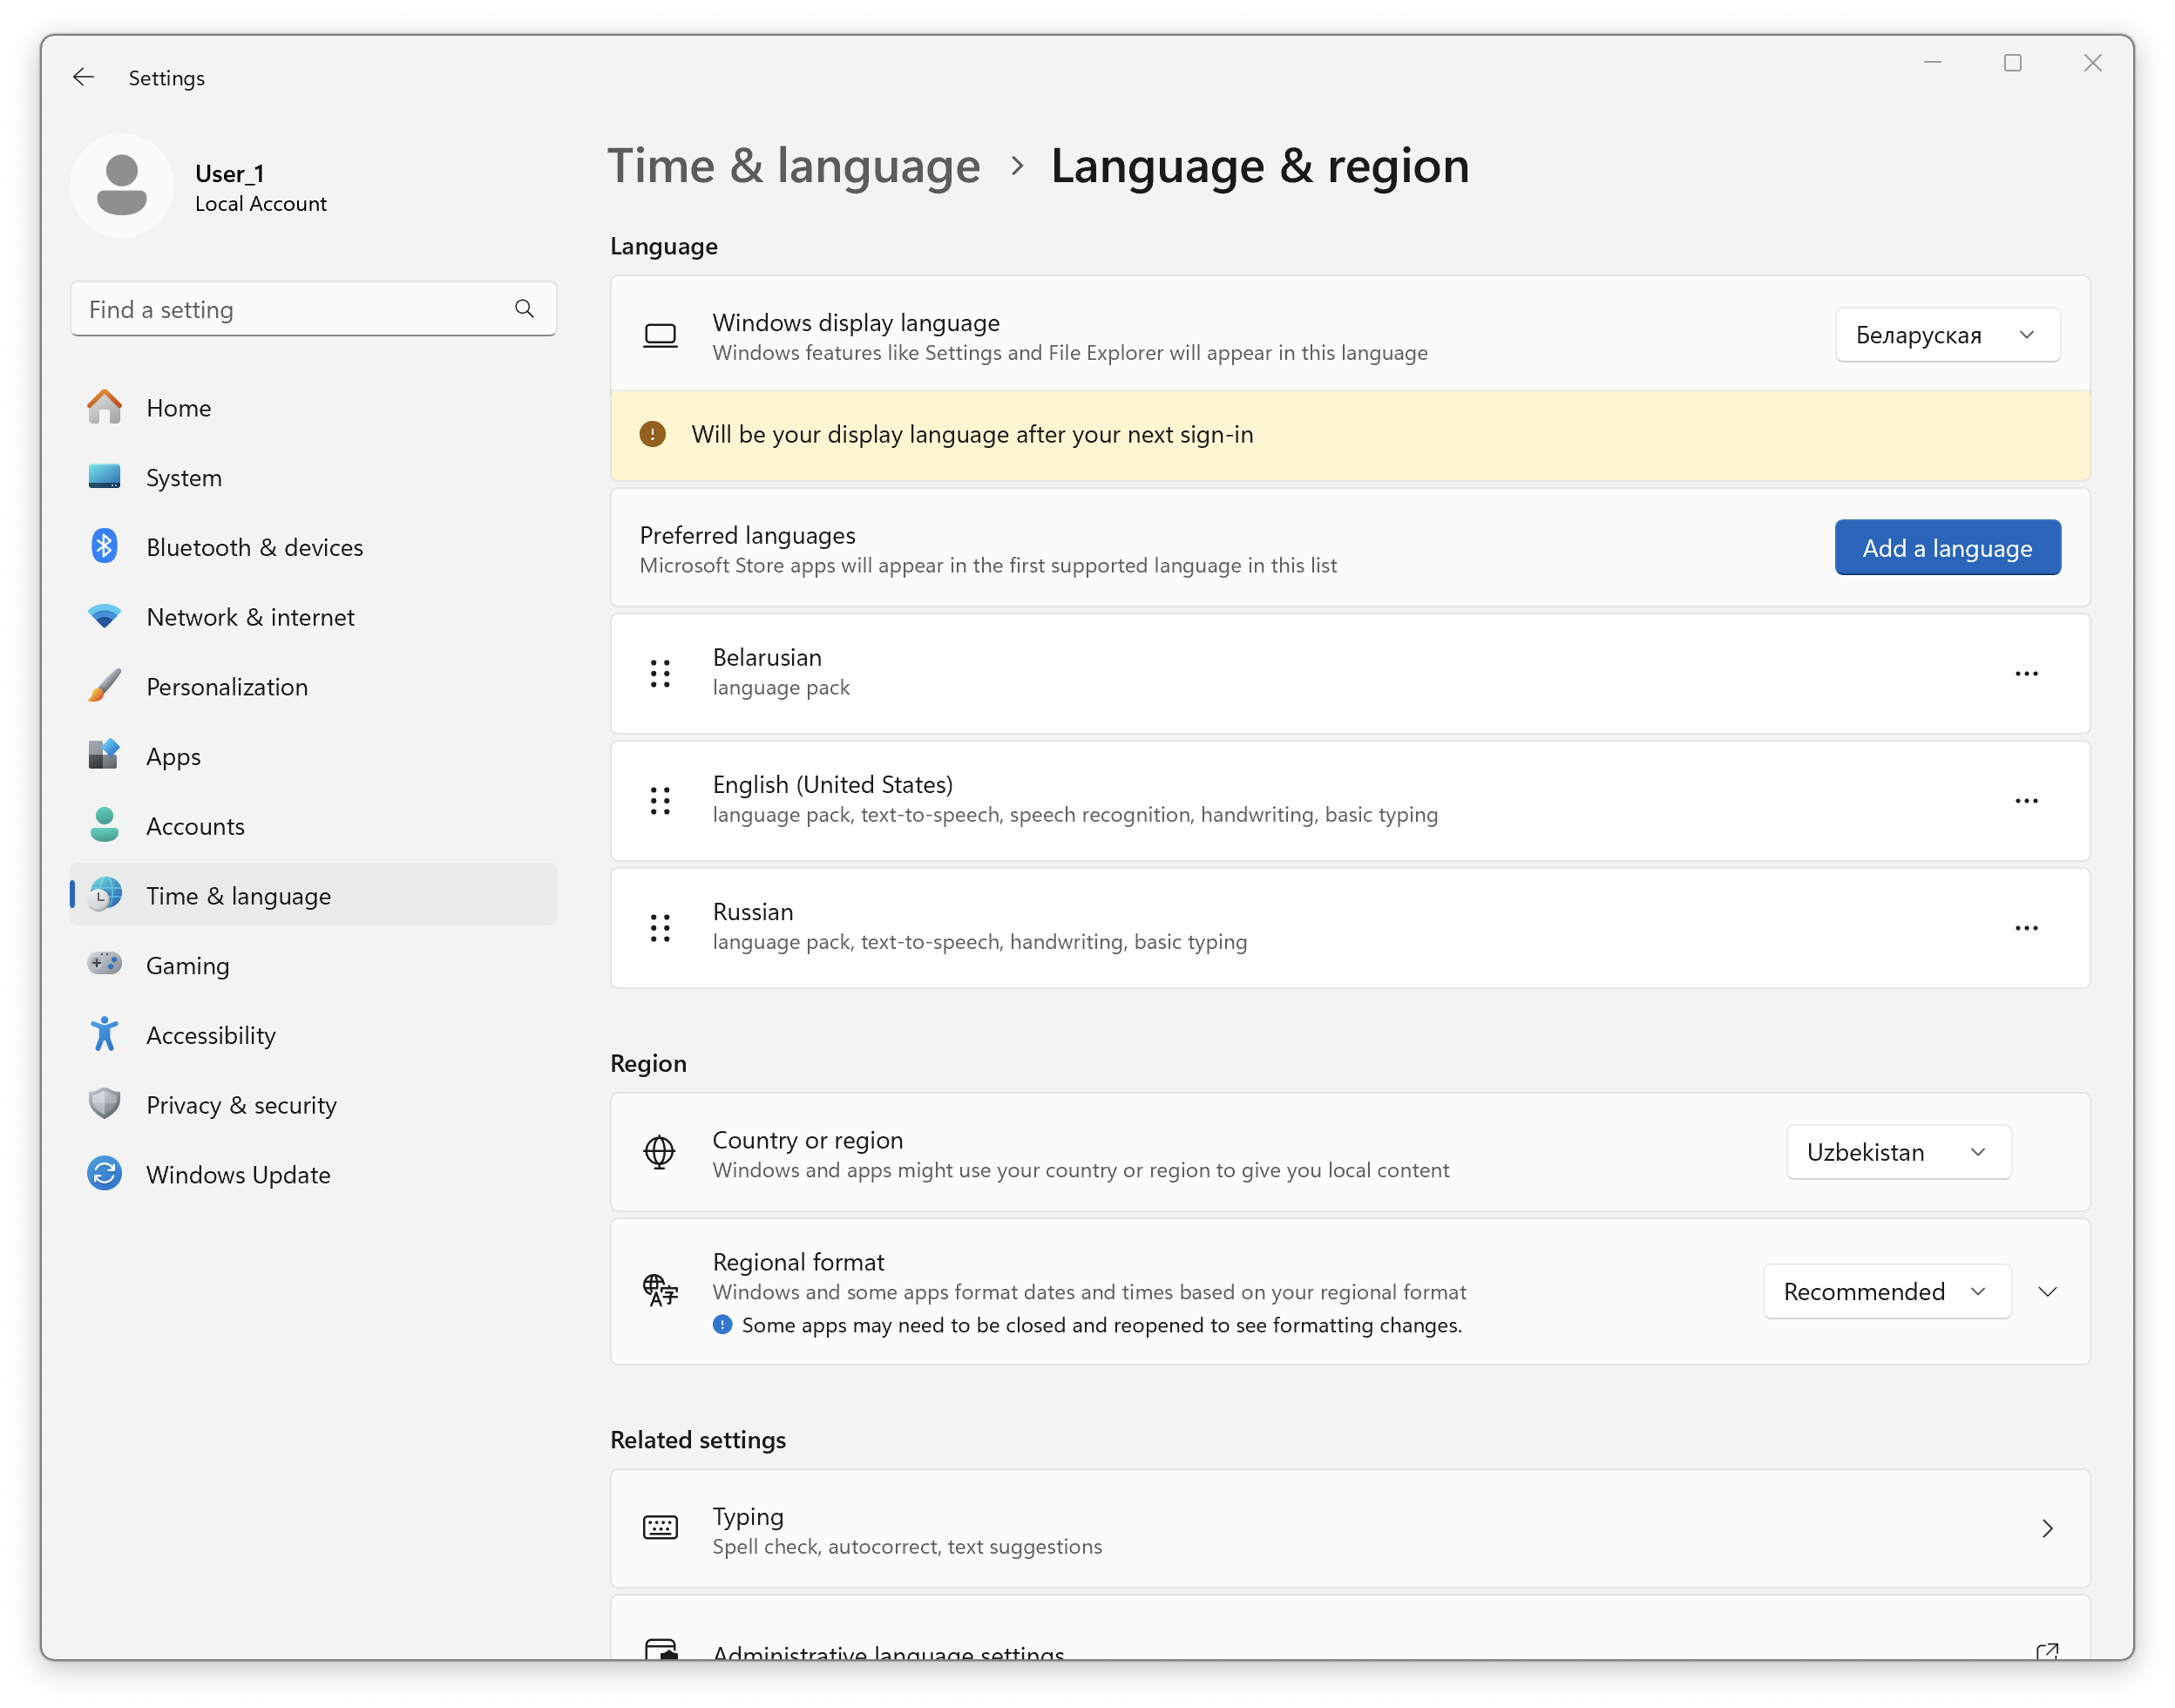
\includegraphics[width=0.8\textwidth]{../images/region_language.png}
              \caption{Настройки региона и языка}
          \end{figure}
          }
    \item {Пользователь может менять параметры персонализации. Например изменить тему оформления.
          \begin{figure}[H]
              \centering
              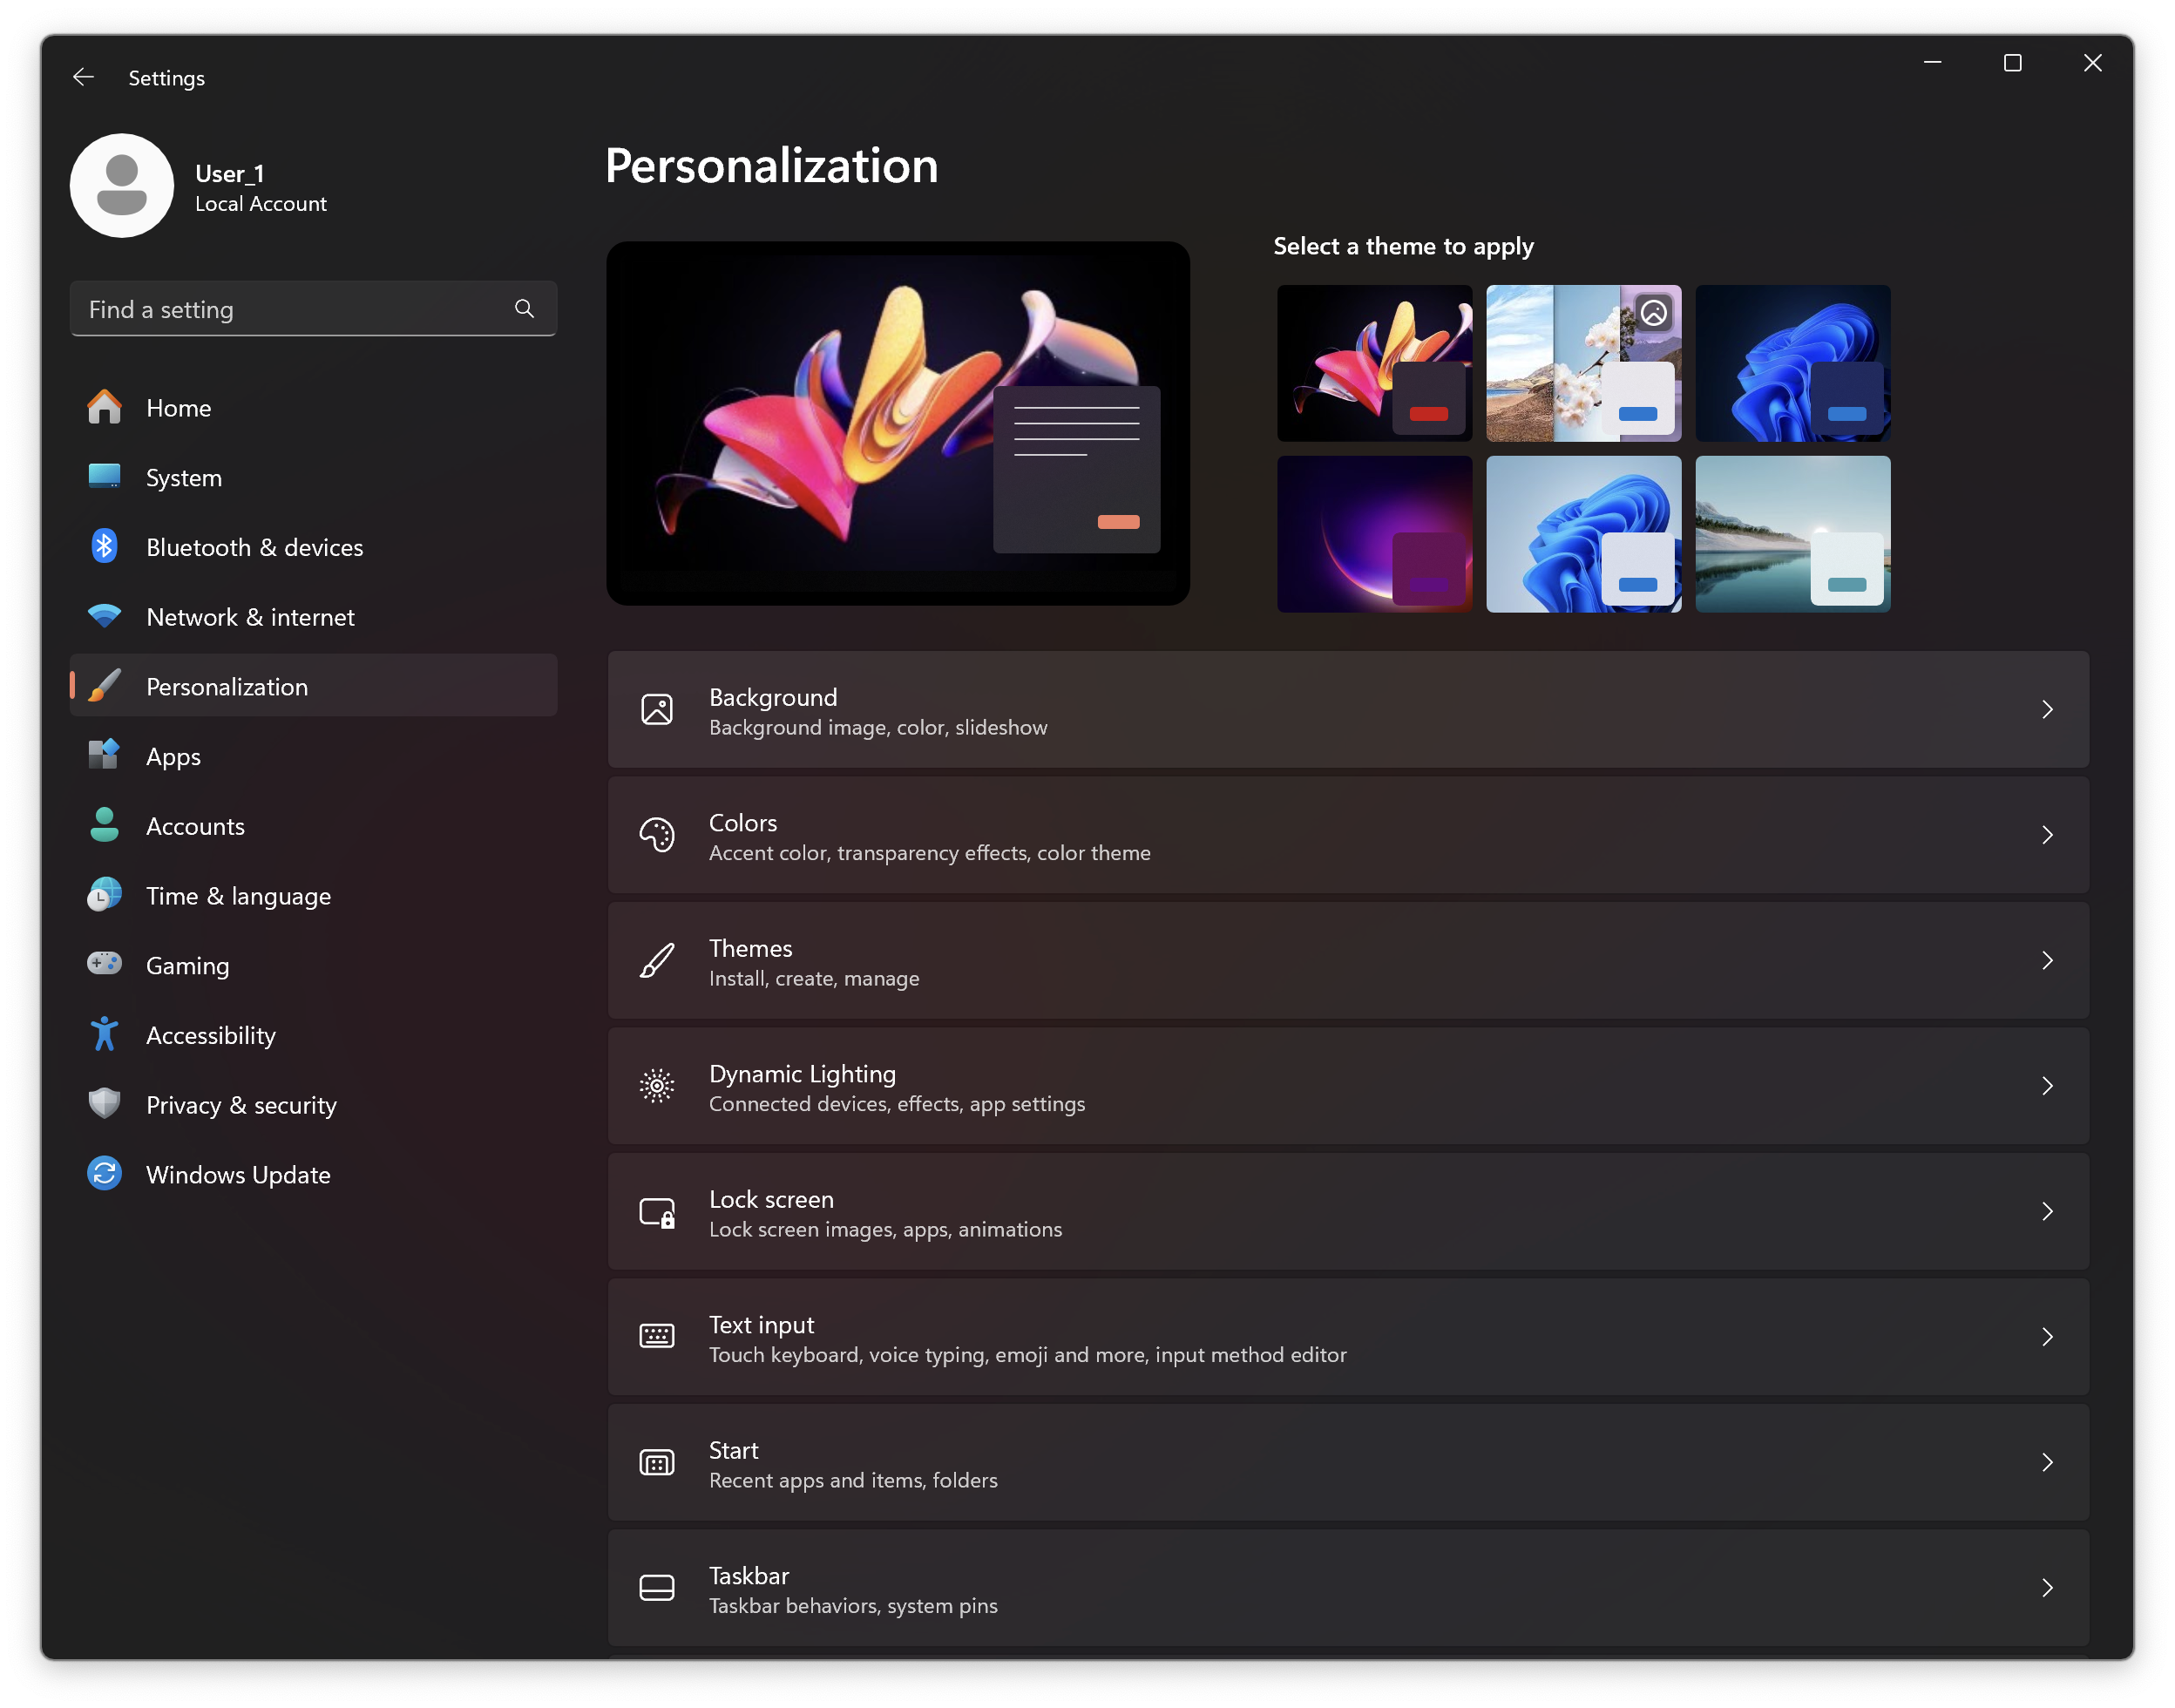
\includegraphics[width=0.8\textwidth]{../images/personalization.png}
              \caption{Персонализация}
          \end{figure}
          }
    \item {Пользователь может изменять параметры Accessibility. Например увеличить шрифт.
          \begin{figure}[H]
              \centering
              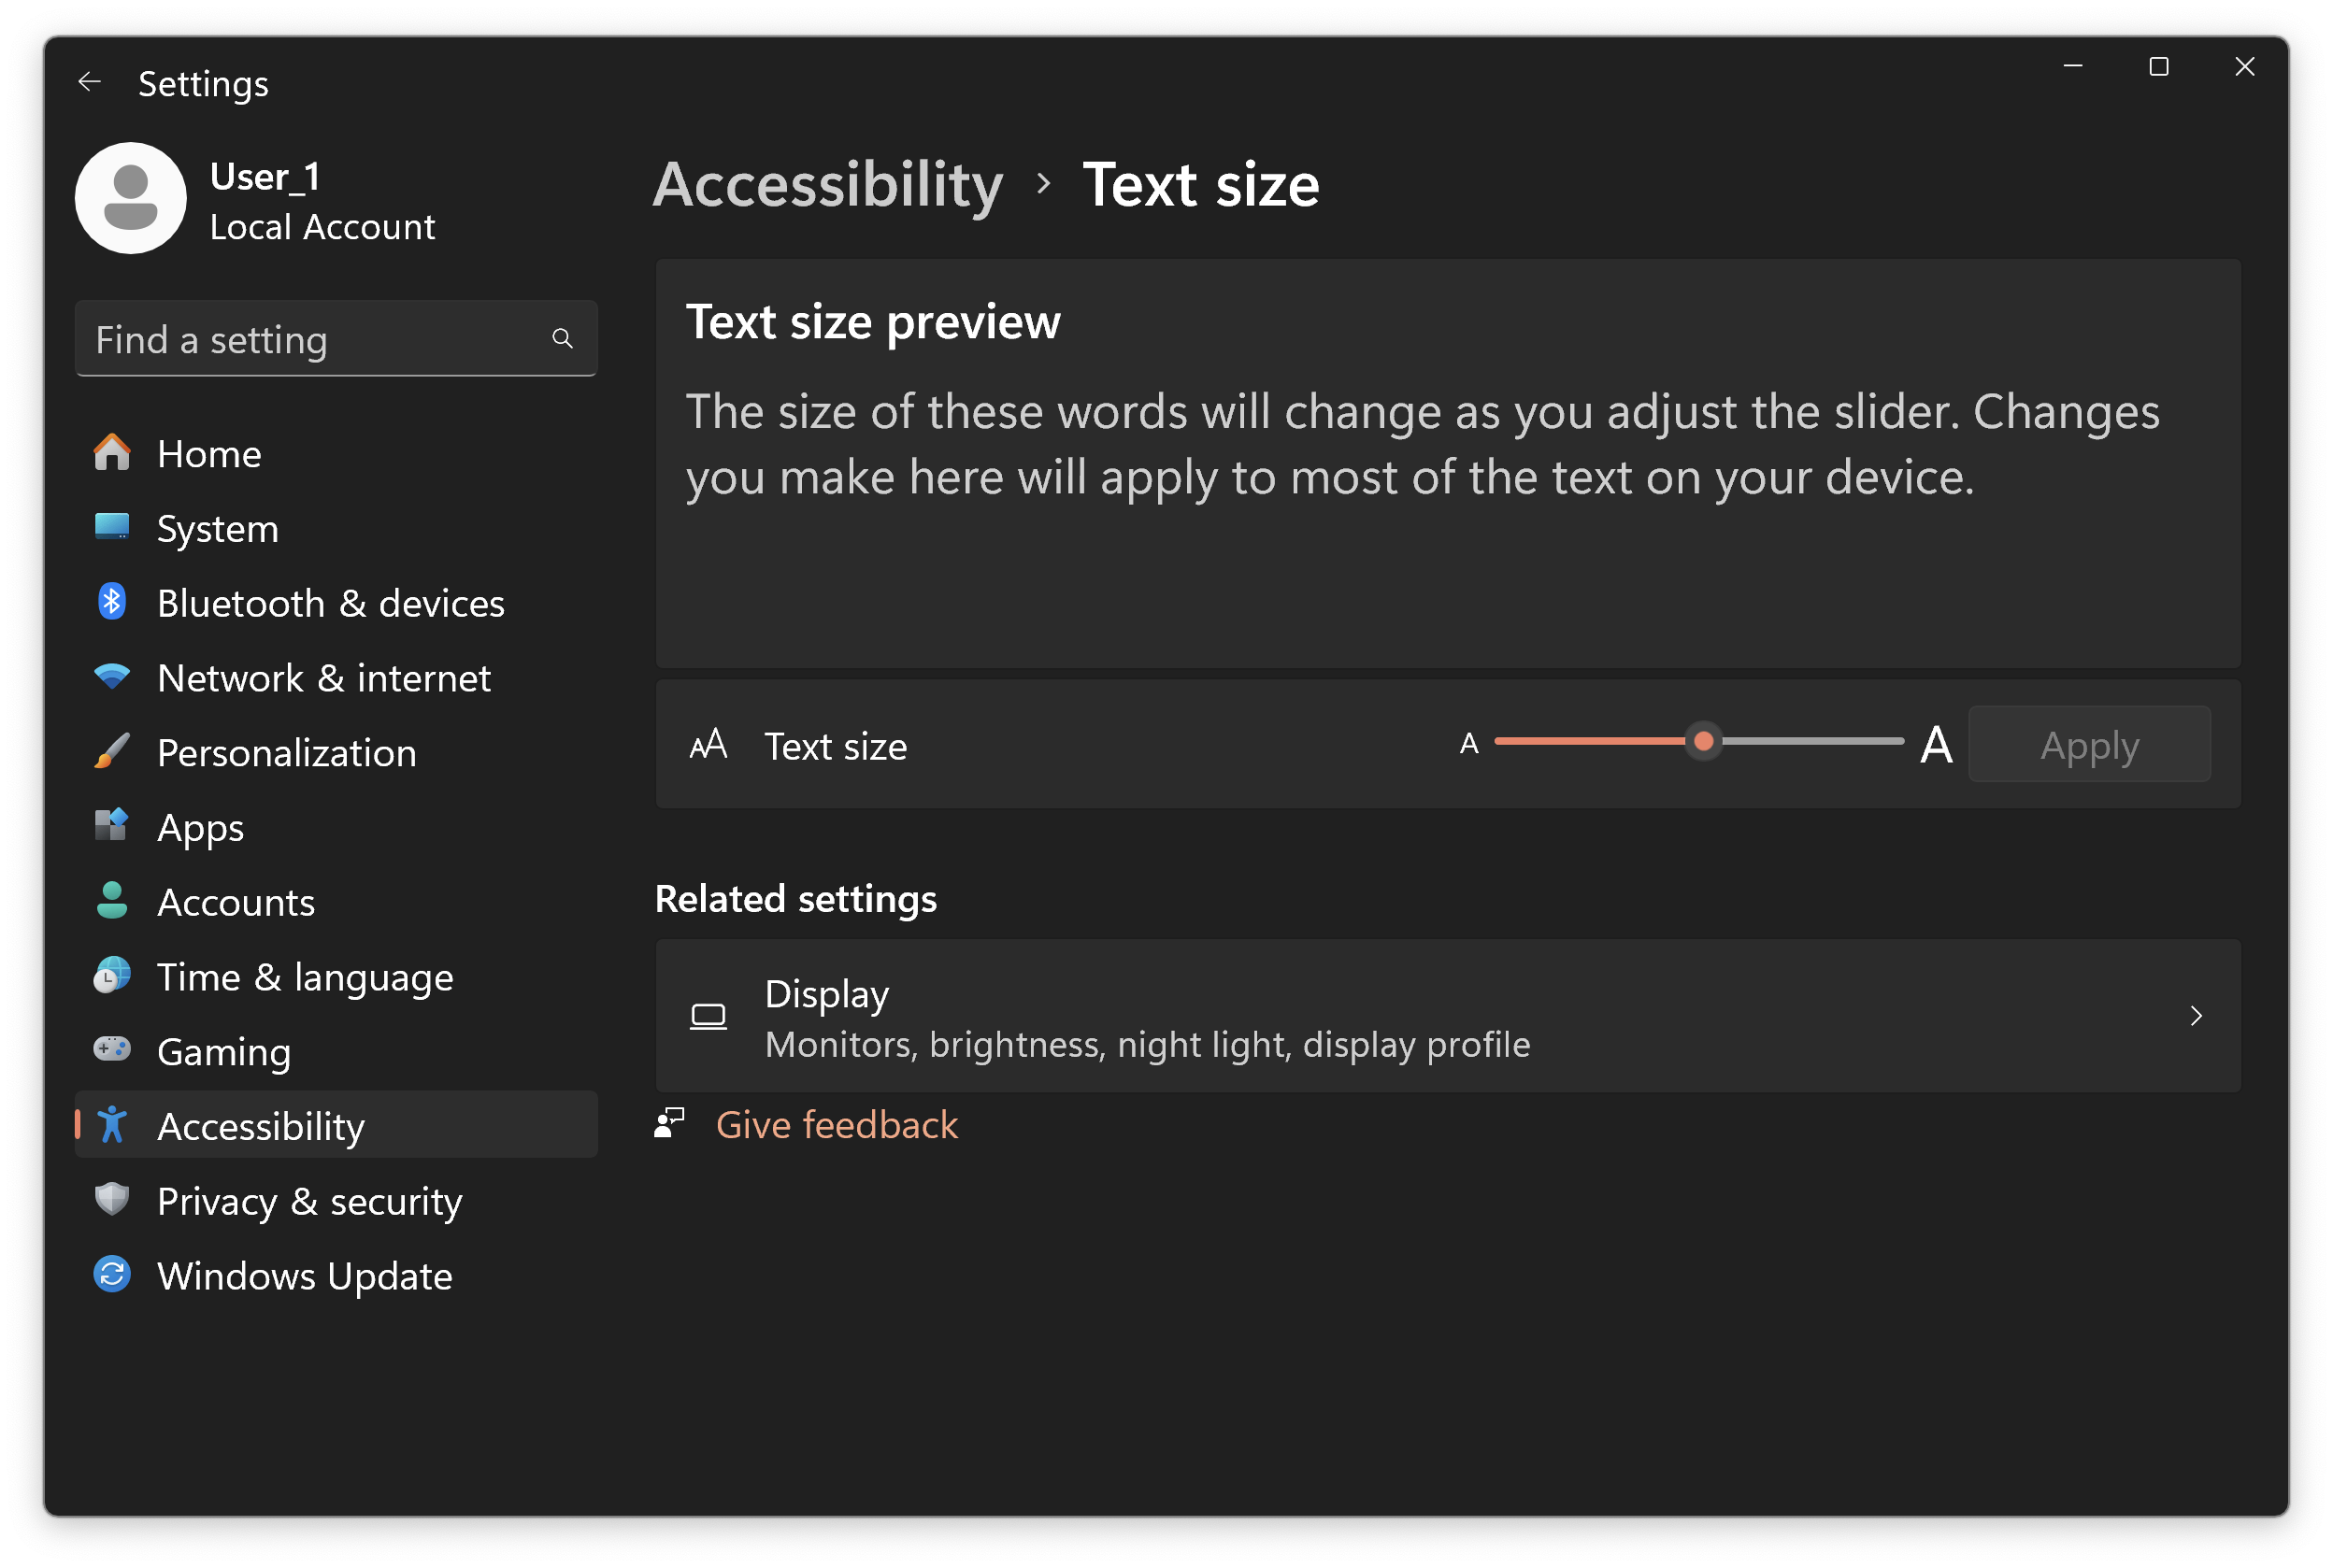
\includegraphics[width=0.8\textwidth]{../images/accessibility.png}
              \caption{Accessibility}
          \end{figure}
          }
    \item {Пользователь может удалять приложения, установленные на компьютере.
          \begin{figure}[H]
              \centering
              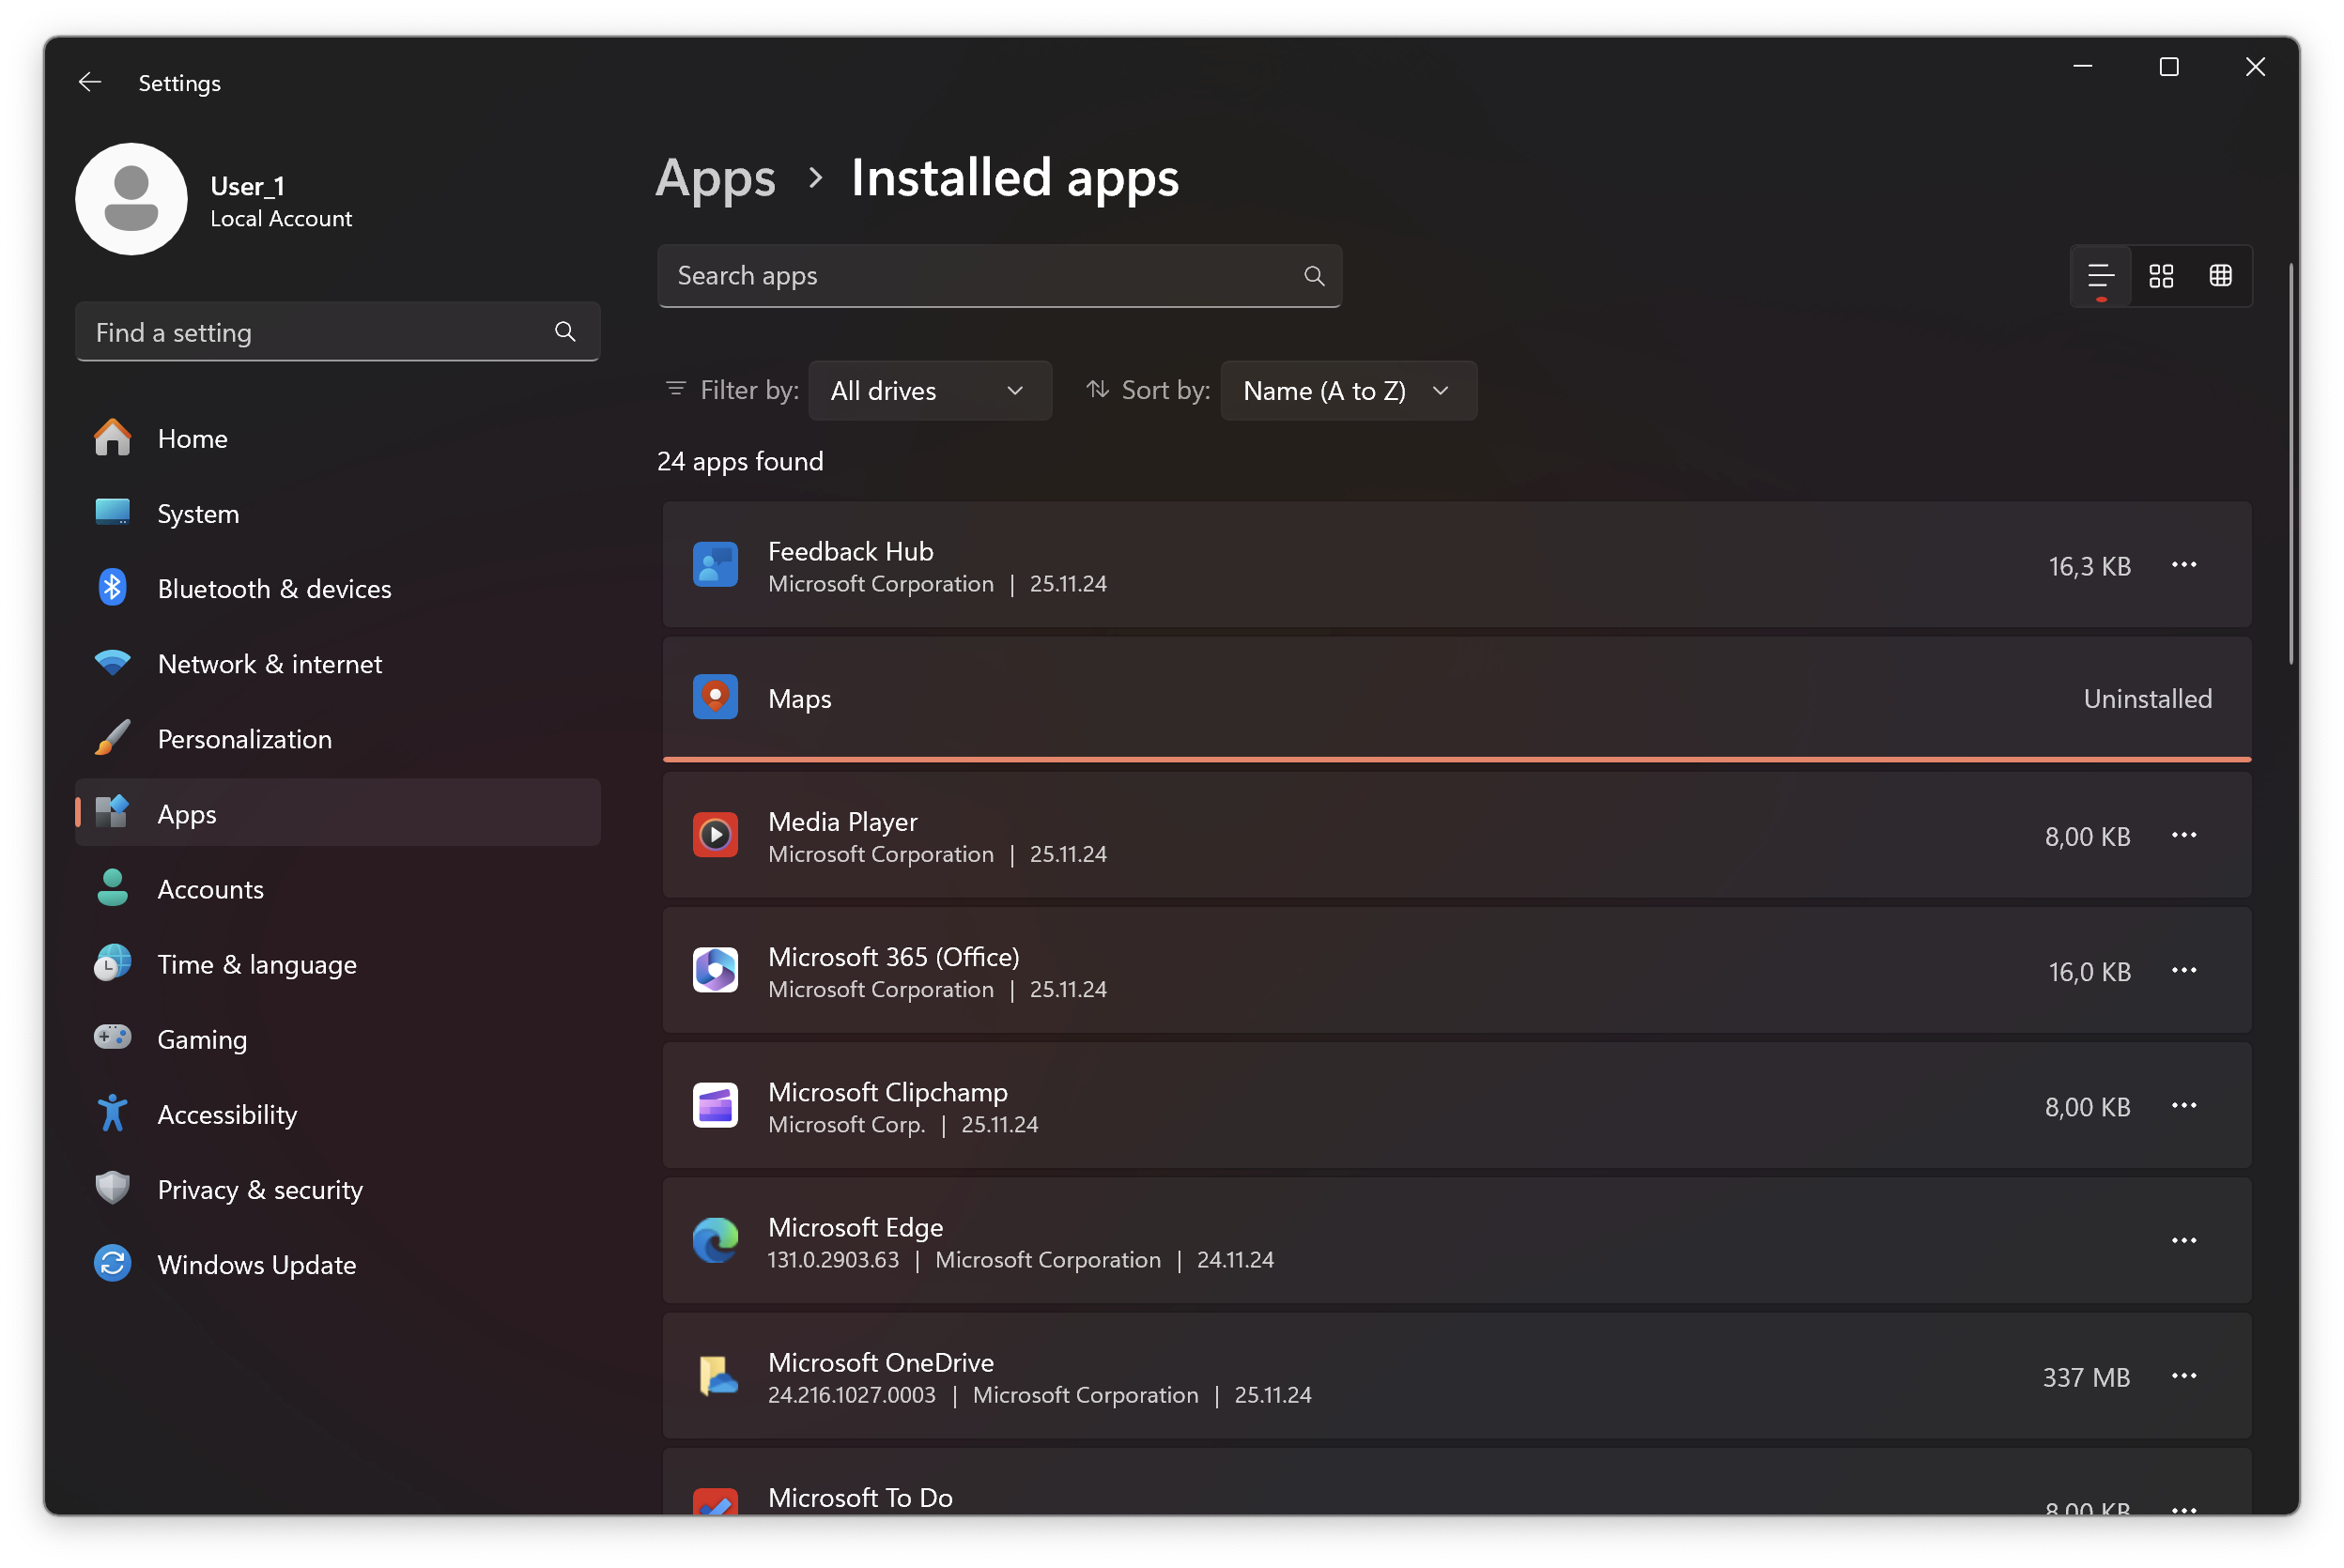
\includegraphics[width=0.8\textwidth]{../images/uninstall_standart_app.png}
              \caption{Удаление приложения}
          \end{figure}
          Однако, пользователь не может удалять приложения, требующие выполнения скриптов.
          \begin{figure}[H]
              \centering
              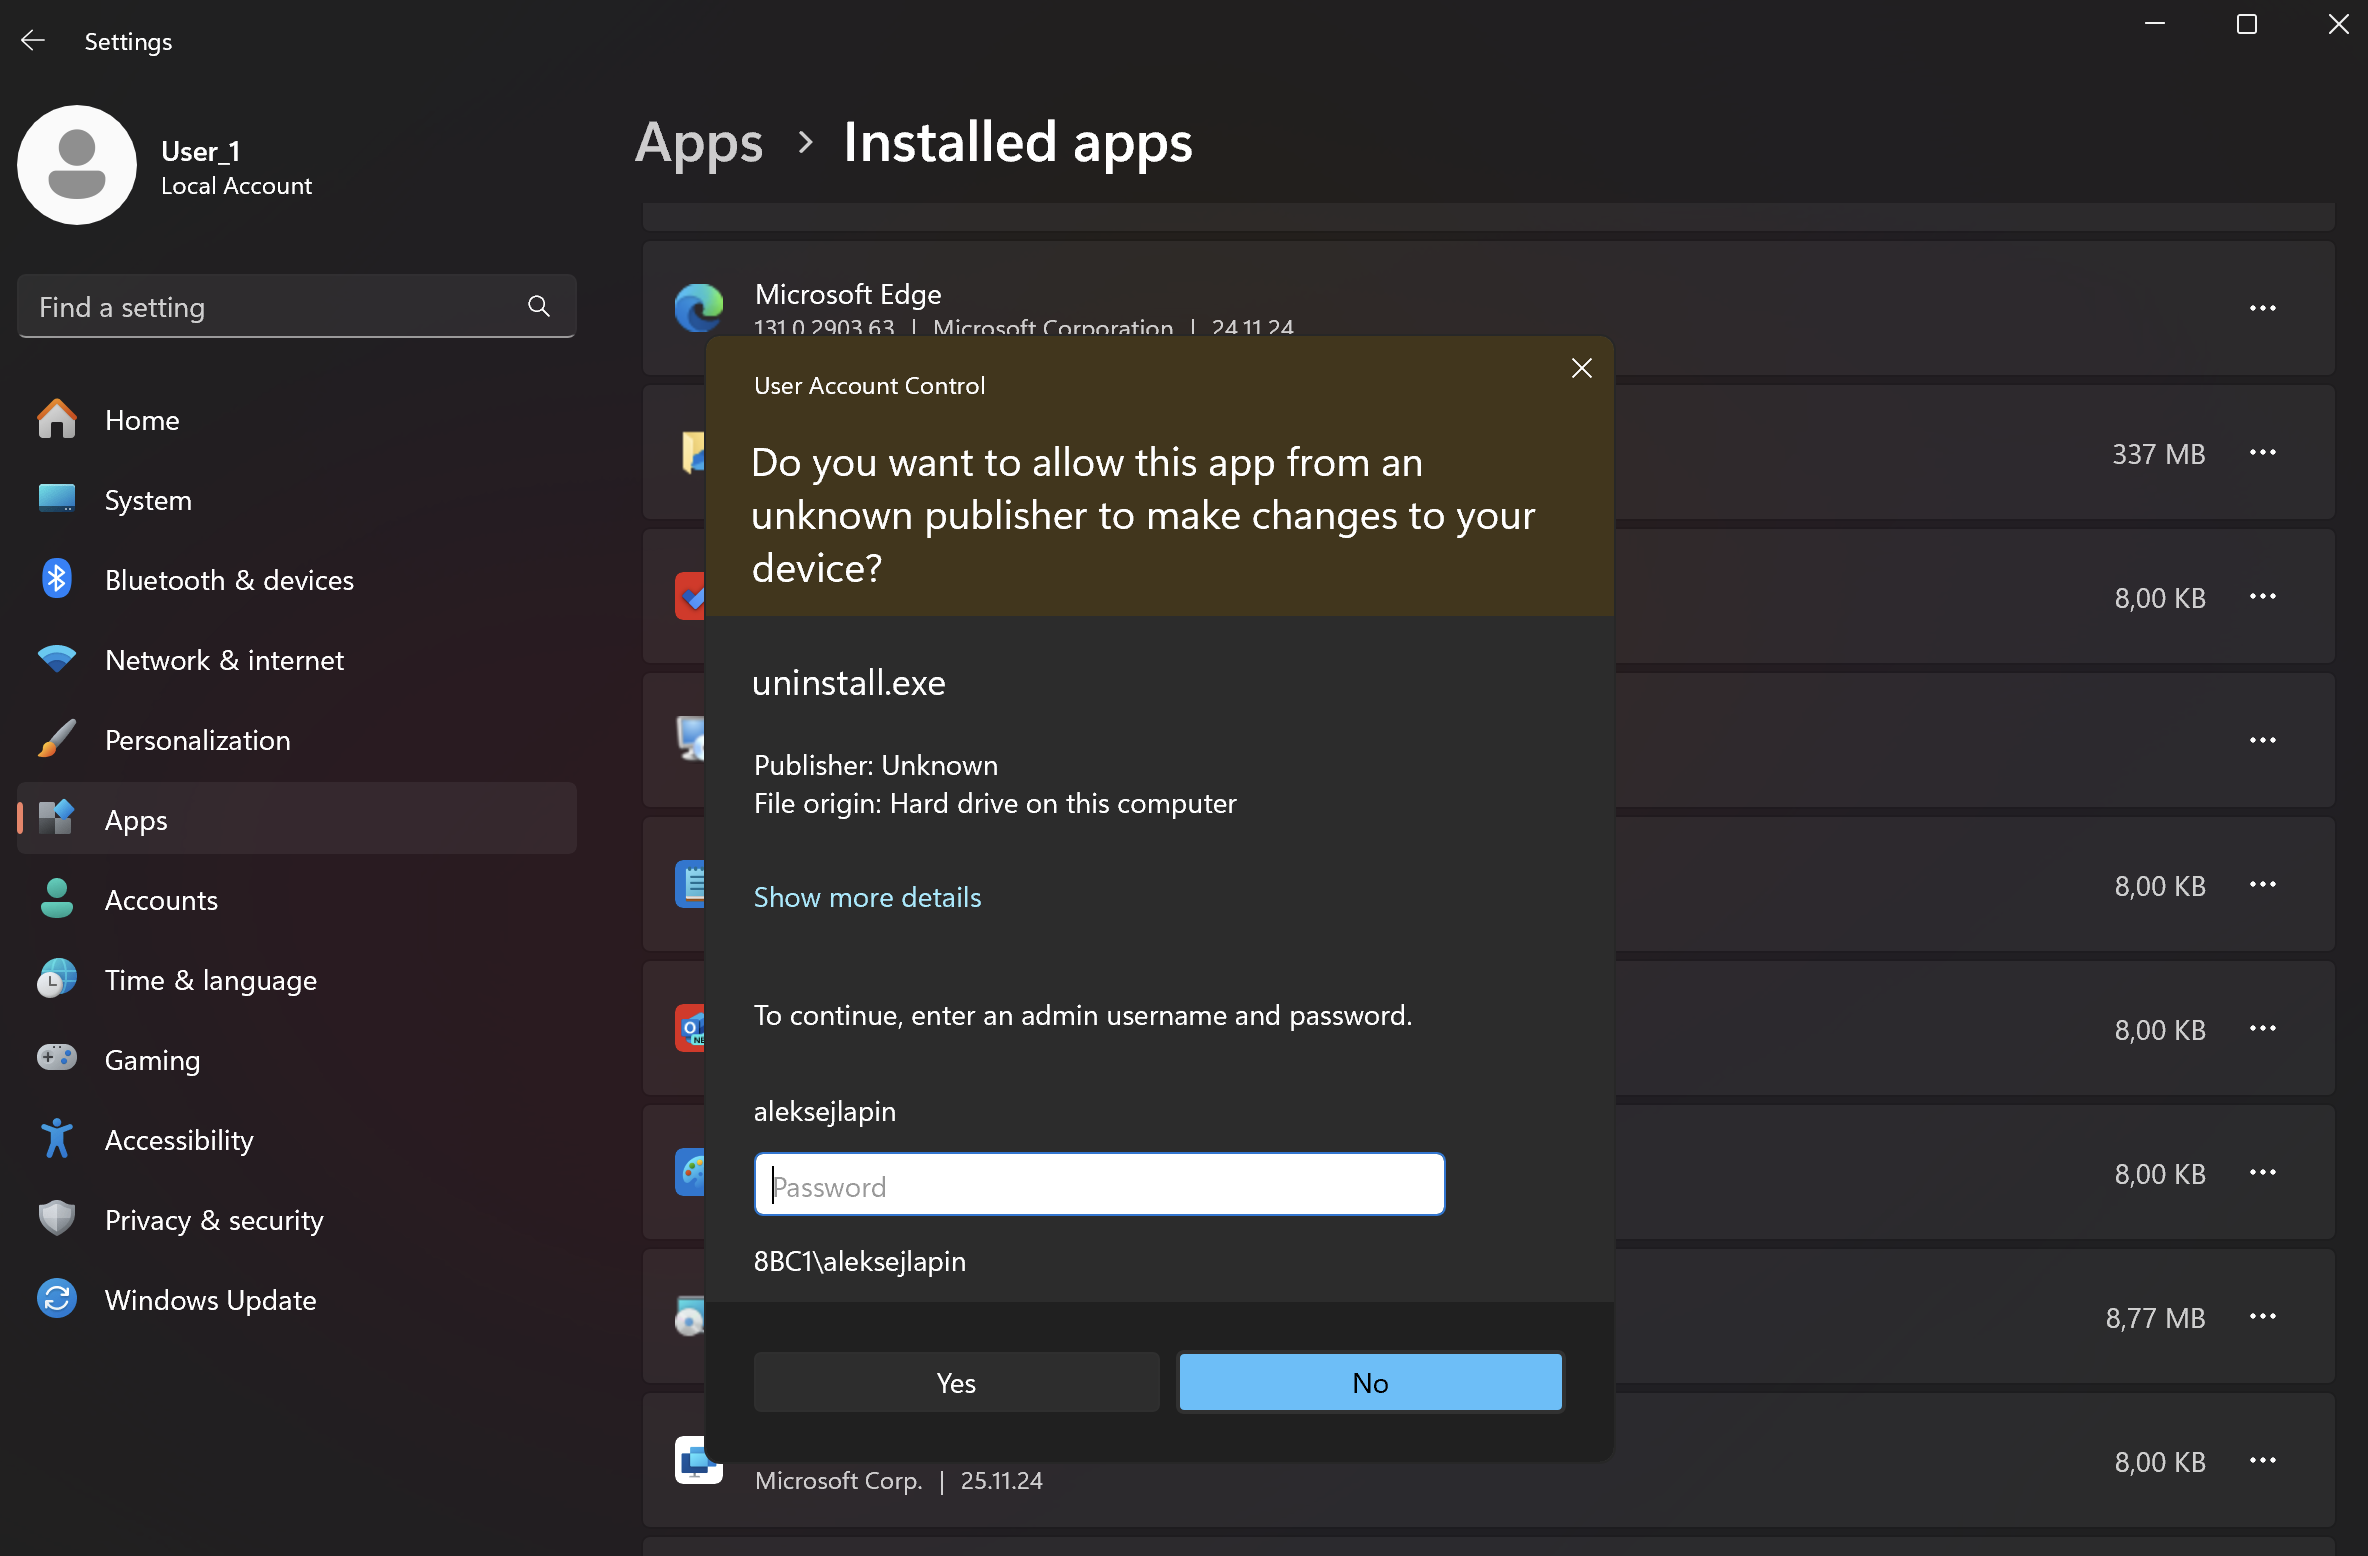
\includegraphics[width=0.8\textwidth]{../images/uninstall_script_app.png}
              \caption{Удаление приложения, требующего выполнения скриптов}
          \end{figure}
          Также, пользователь не может получить доступ к папкам, других пользователей.
          \begin{figure}[H]
              \centering
              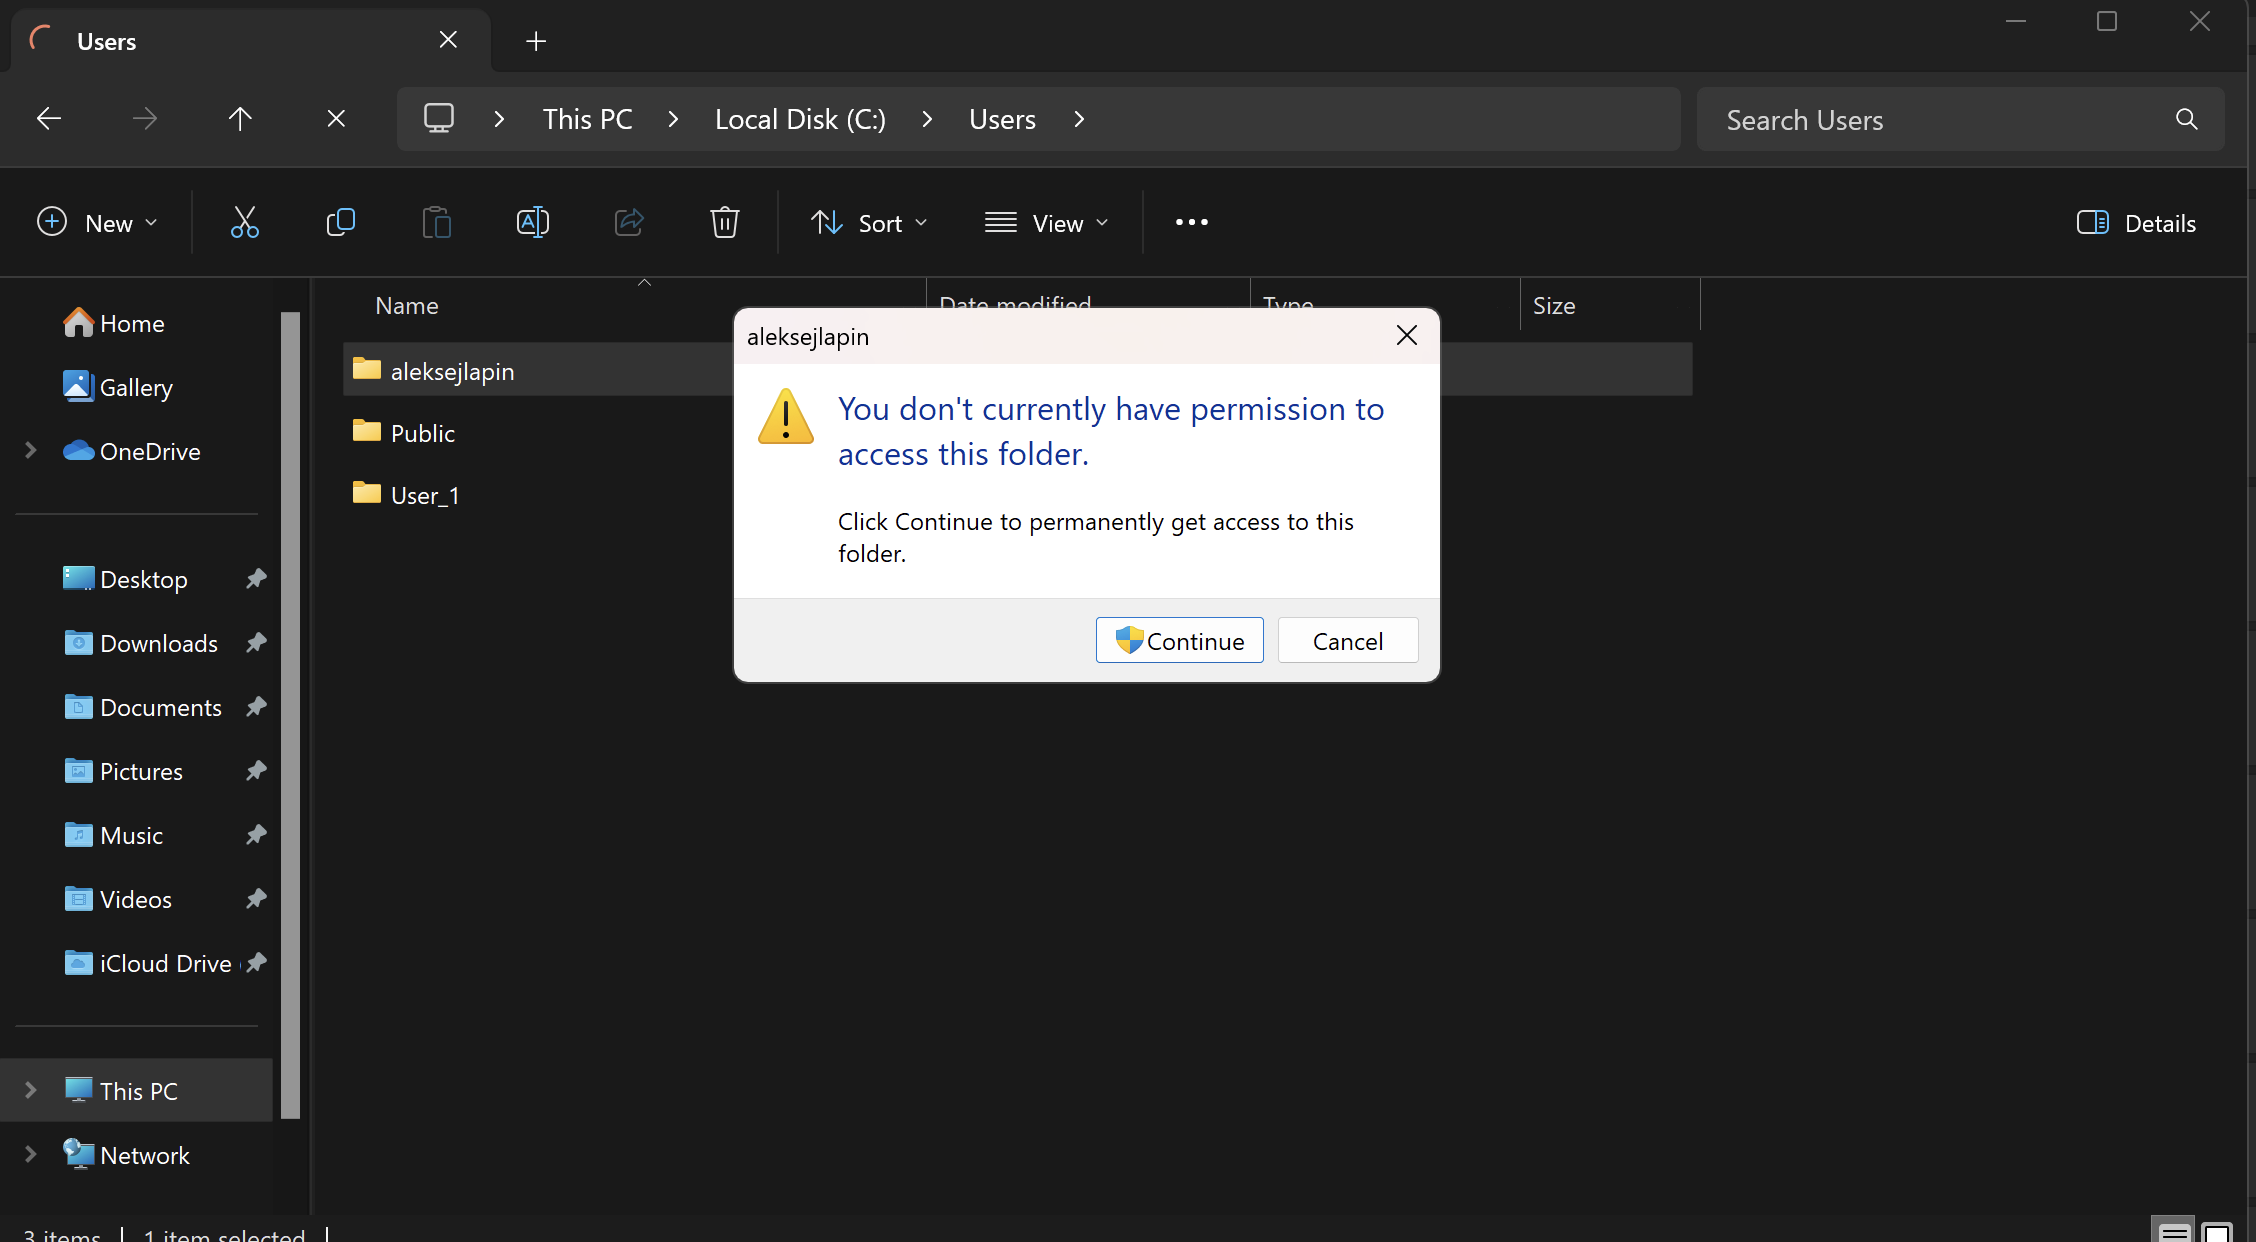
\includegraphics[width=0.8\textwidth]{../images/others_folder.png}
              \caption{Доступ к папкам других пользователей}
          \end{figure}
          Также, пользователь не может получить доступ к некоторым системамным папкам.
          \begin{figure}[H]
              \centering
              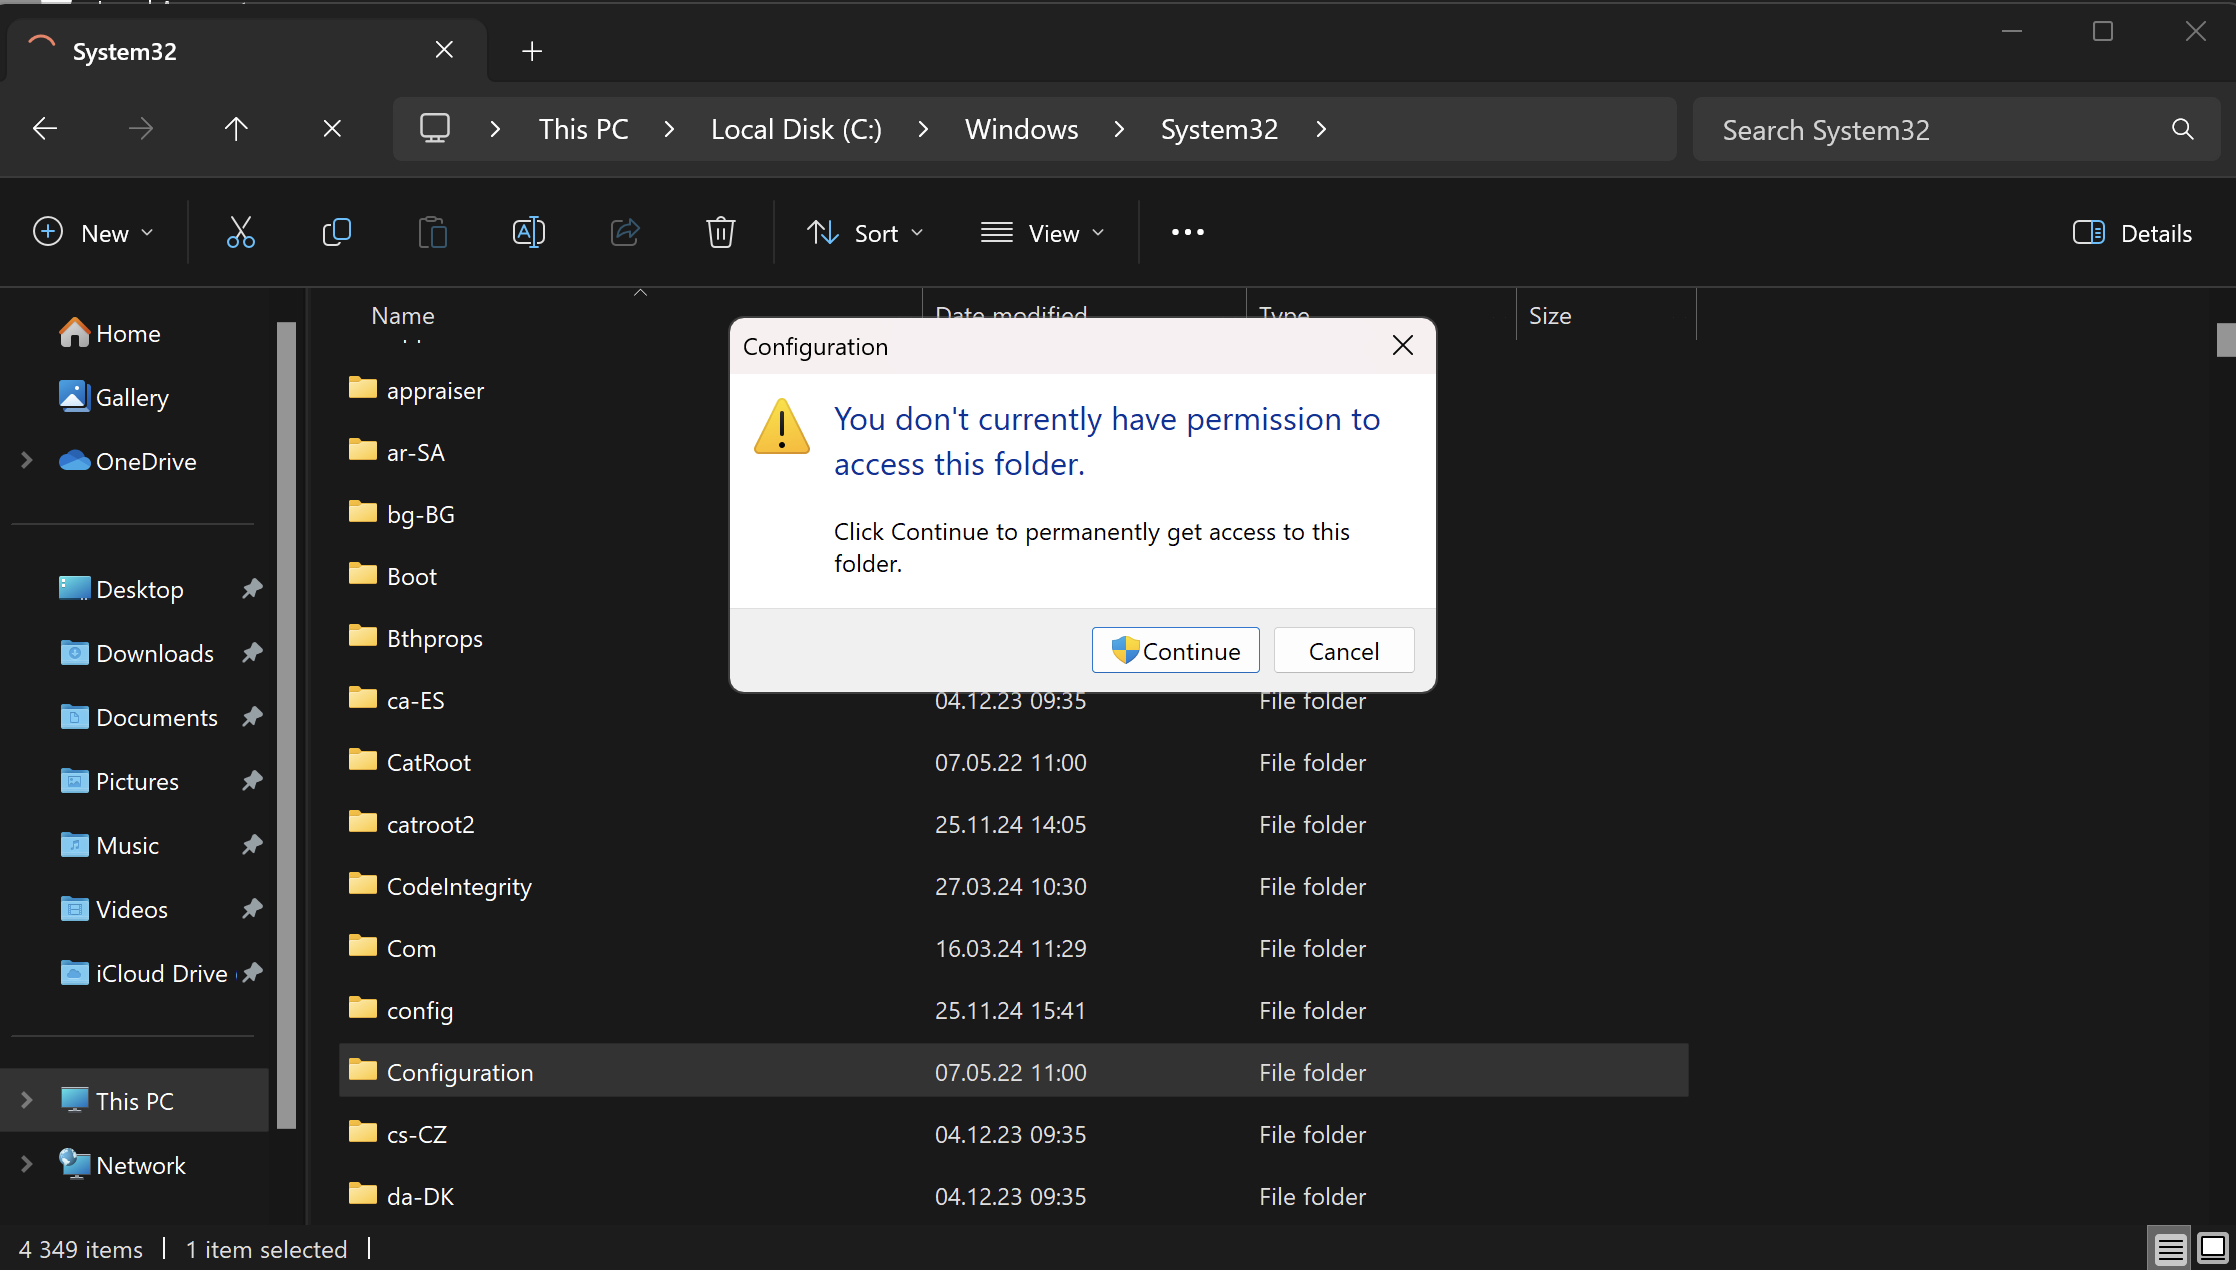
\includegraphics[width=0.8\textwidth]{../images/system_folder.png}
              \caption{Доступ к системной папке}
          \end{figure}
          }
\end{enumerate}
\section{Создание администратора}
\nsubsection{Вариант 1. Создание администратора в Параметрах Windows 11}
\begin{enumerate}
    \item Создадим нового пользователя аналогично варианту 1 из предыдущего пункта.
    \item Нажмем правой кнопкой мыши на пользователя и выберем "Изменить учетную запись".
    \item Выберем "Администратор".
          {
          \begin{figure}[H]
              \centering
              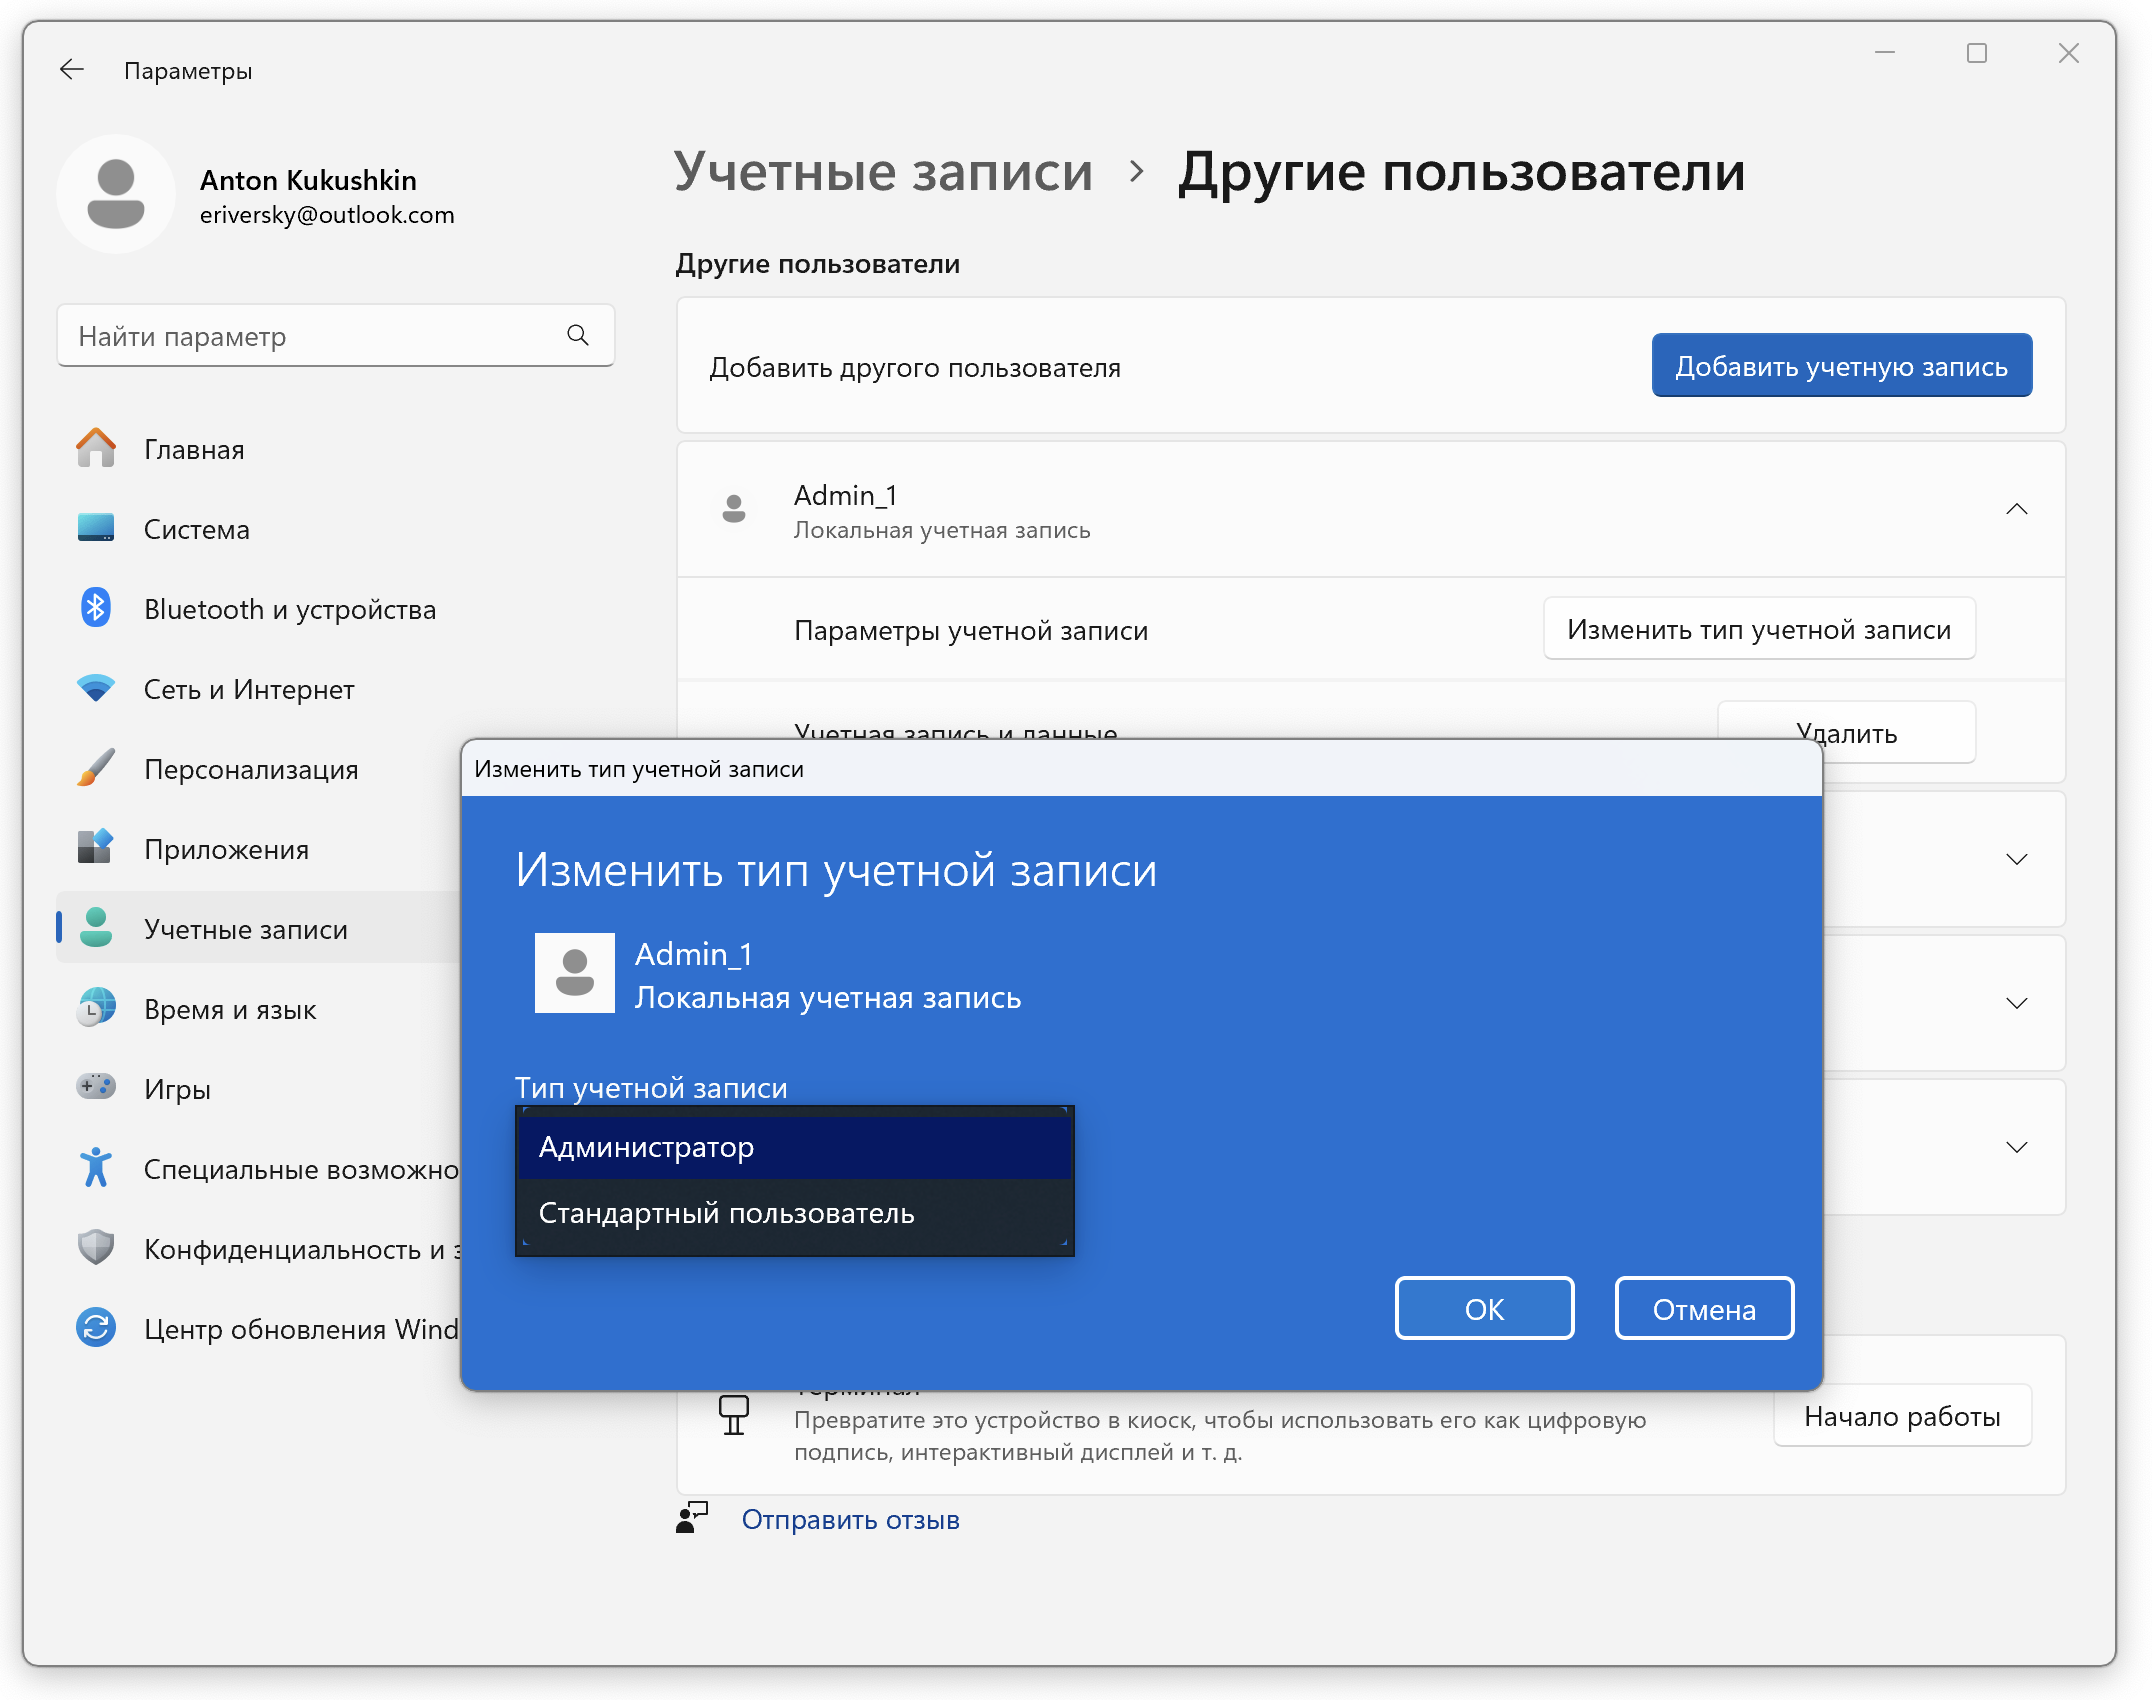
\includegraphics[width=0.8\textwidth]{../images/create_admin.png}
              \caption{Создание администратора}
          \end{figure}
          }
\end{enumerate}
\nsubsection{Вариант 2. Создание администратора в Управлении учетными записями пользователей}
\begin{enumerate}
    \item Создадим нового пользователя аналогично варианту 3 из предыдущего пункта.
    \item Переходим в раздел «Группы».
    \item Нажмем правой кнопкой мыши на группу «Администраторы» и выберем "Добавить в группу".
    \item Выберем «Добавить»
    \item Введем имя пользователя и нажмем «ОК».
          {
          \begin{figure}[H]
              \centering
              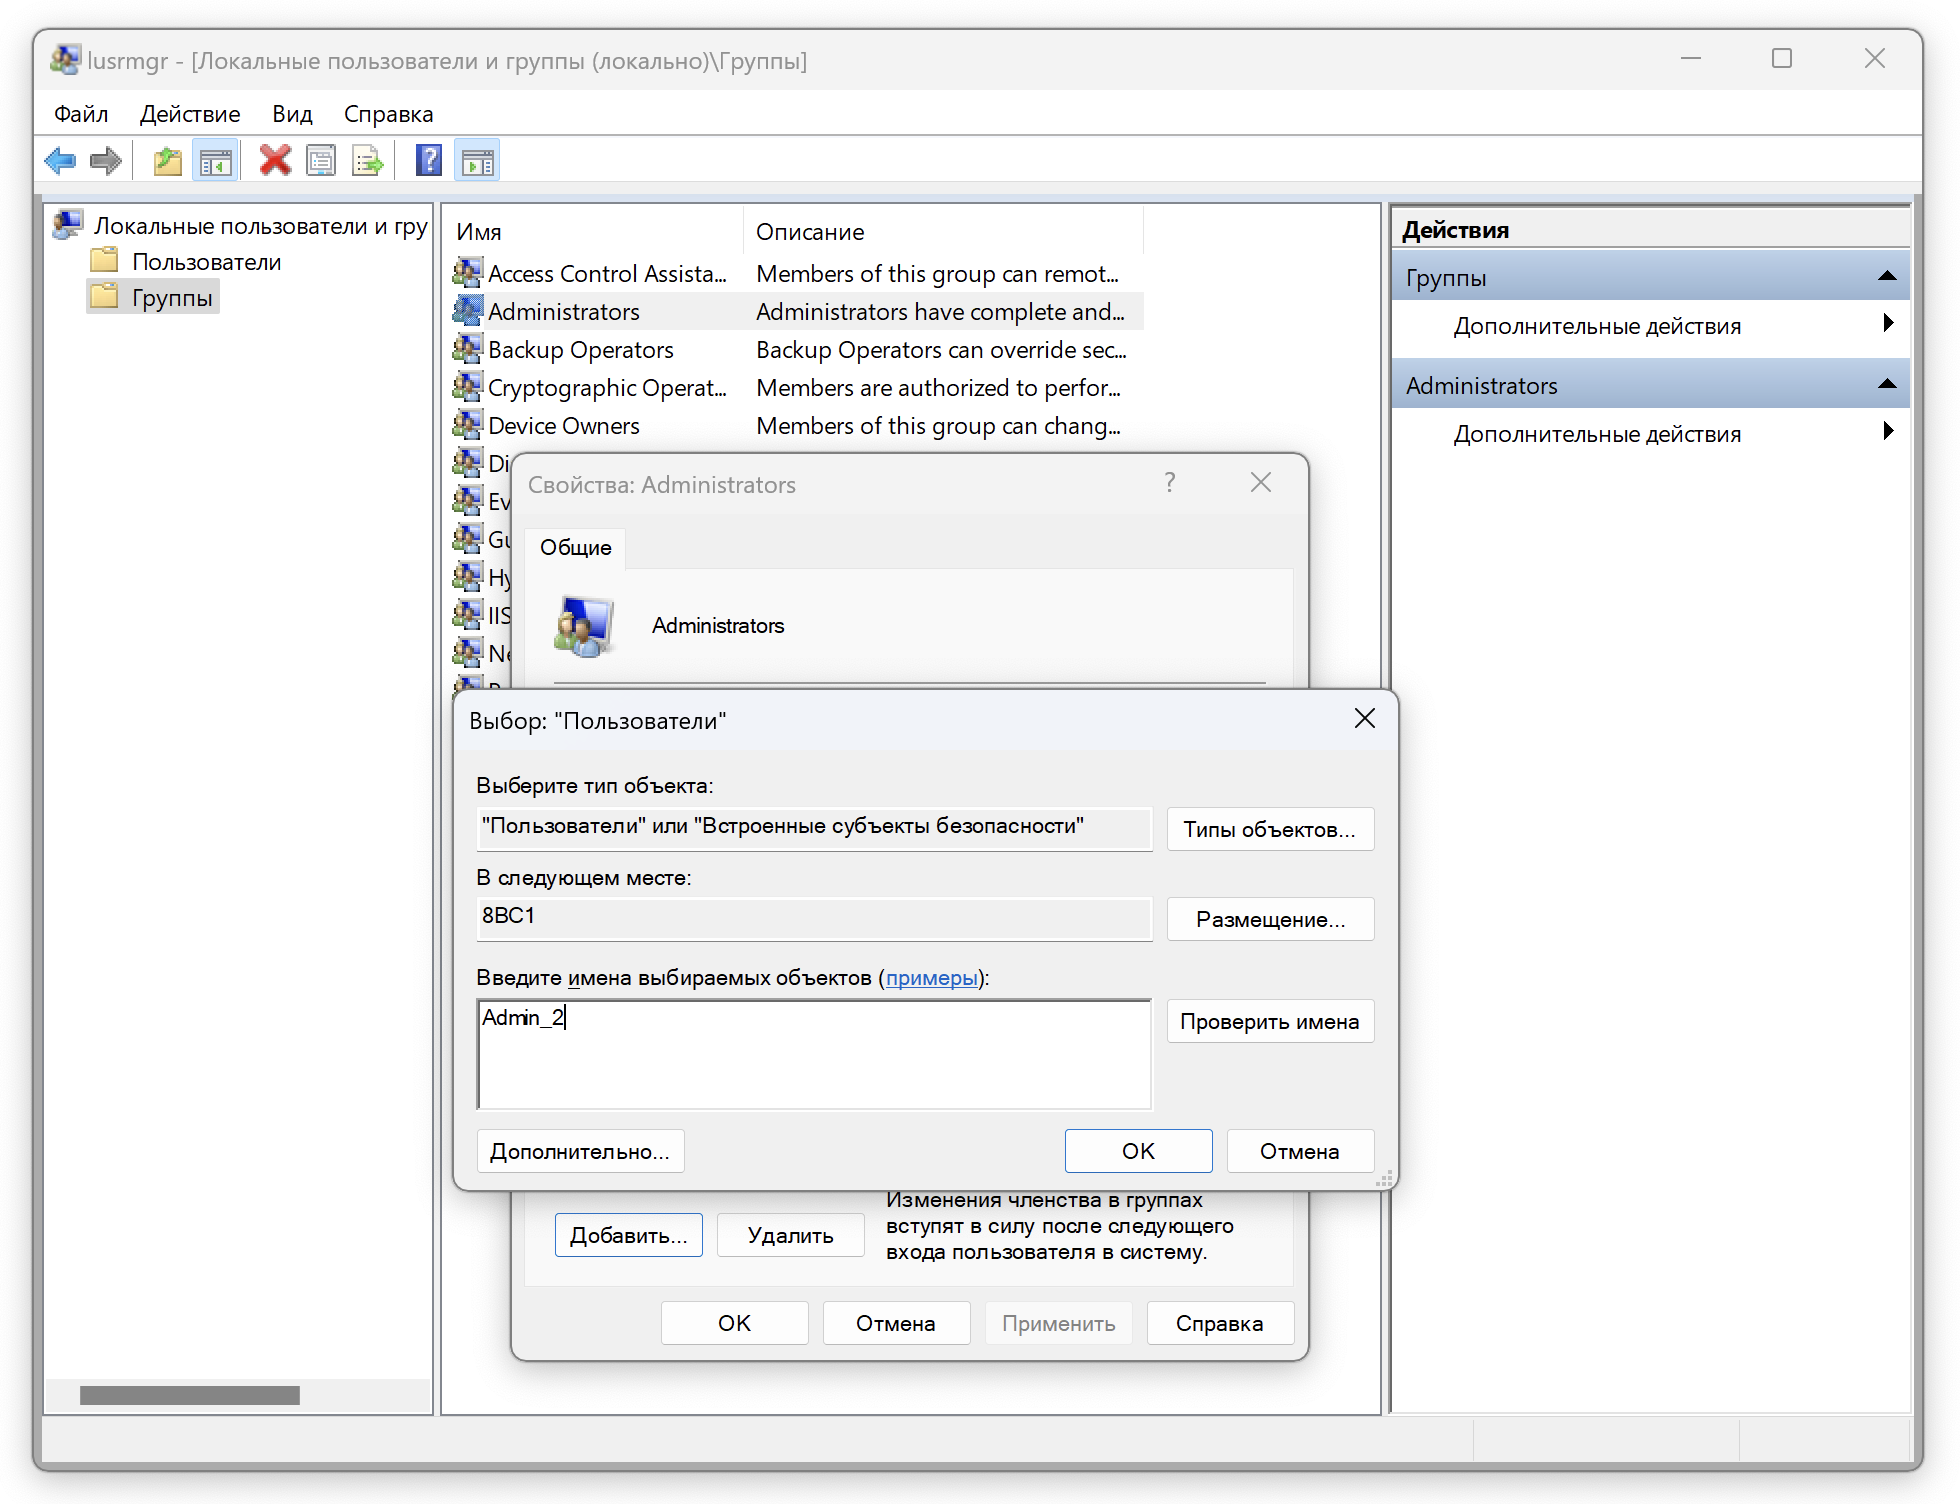
\includegraphics[width=0.8\textwidth]{../images/lusrmgr_create_admin.png}
              \caption{Создание администратора}
          \end{figure}
          }
\end{enumerate}
\nsubsection{Вариант 3. Создание администратора с помощью командной строки}
\begin{enumerate}
    \item Откроем командную строку от имени администратора.
    \item Введем команду \texttt{net user <имя пользователя> /add}
    \item Введем команду \texttt{net localgroup}, чтобы посмотреть доступные группы.
    \item Введем команду \texttt{net localgroup "Administrators" <имя пользователя> /add}
    \item {
          \begin{figure}[H]
              \centering
              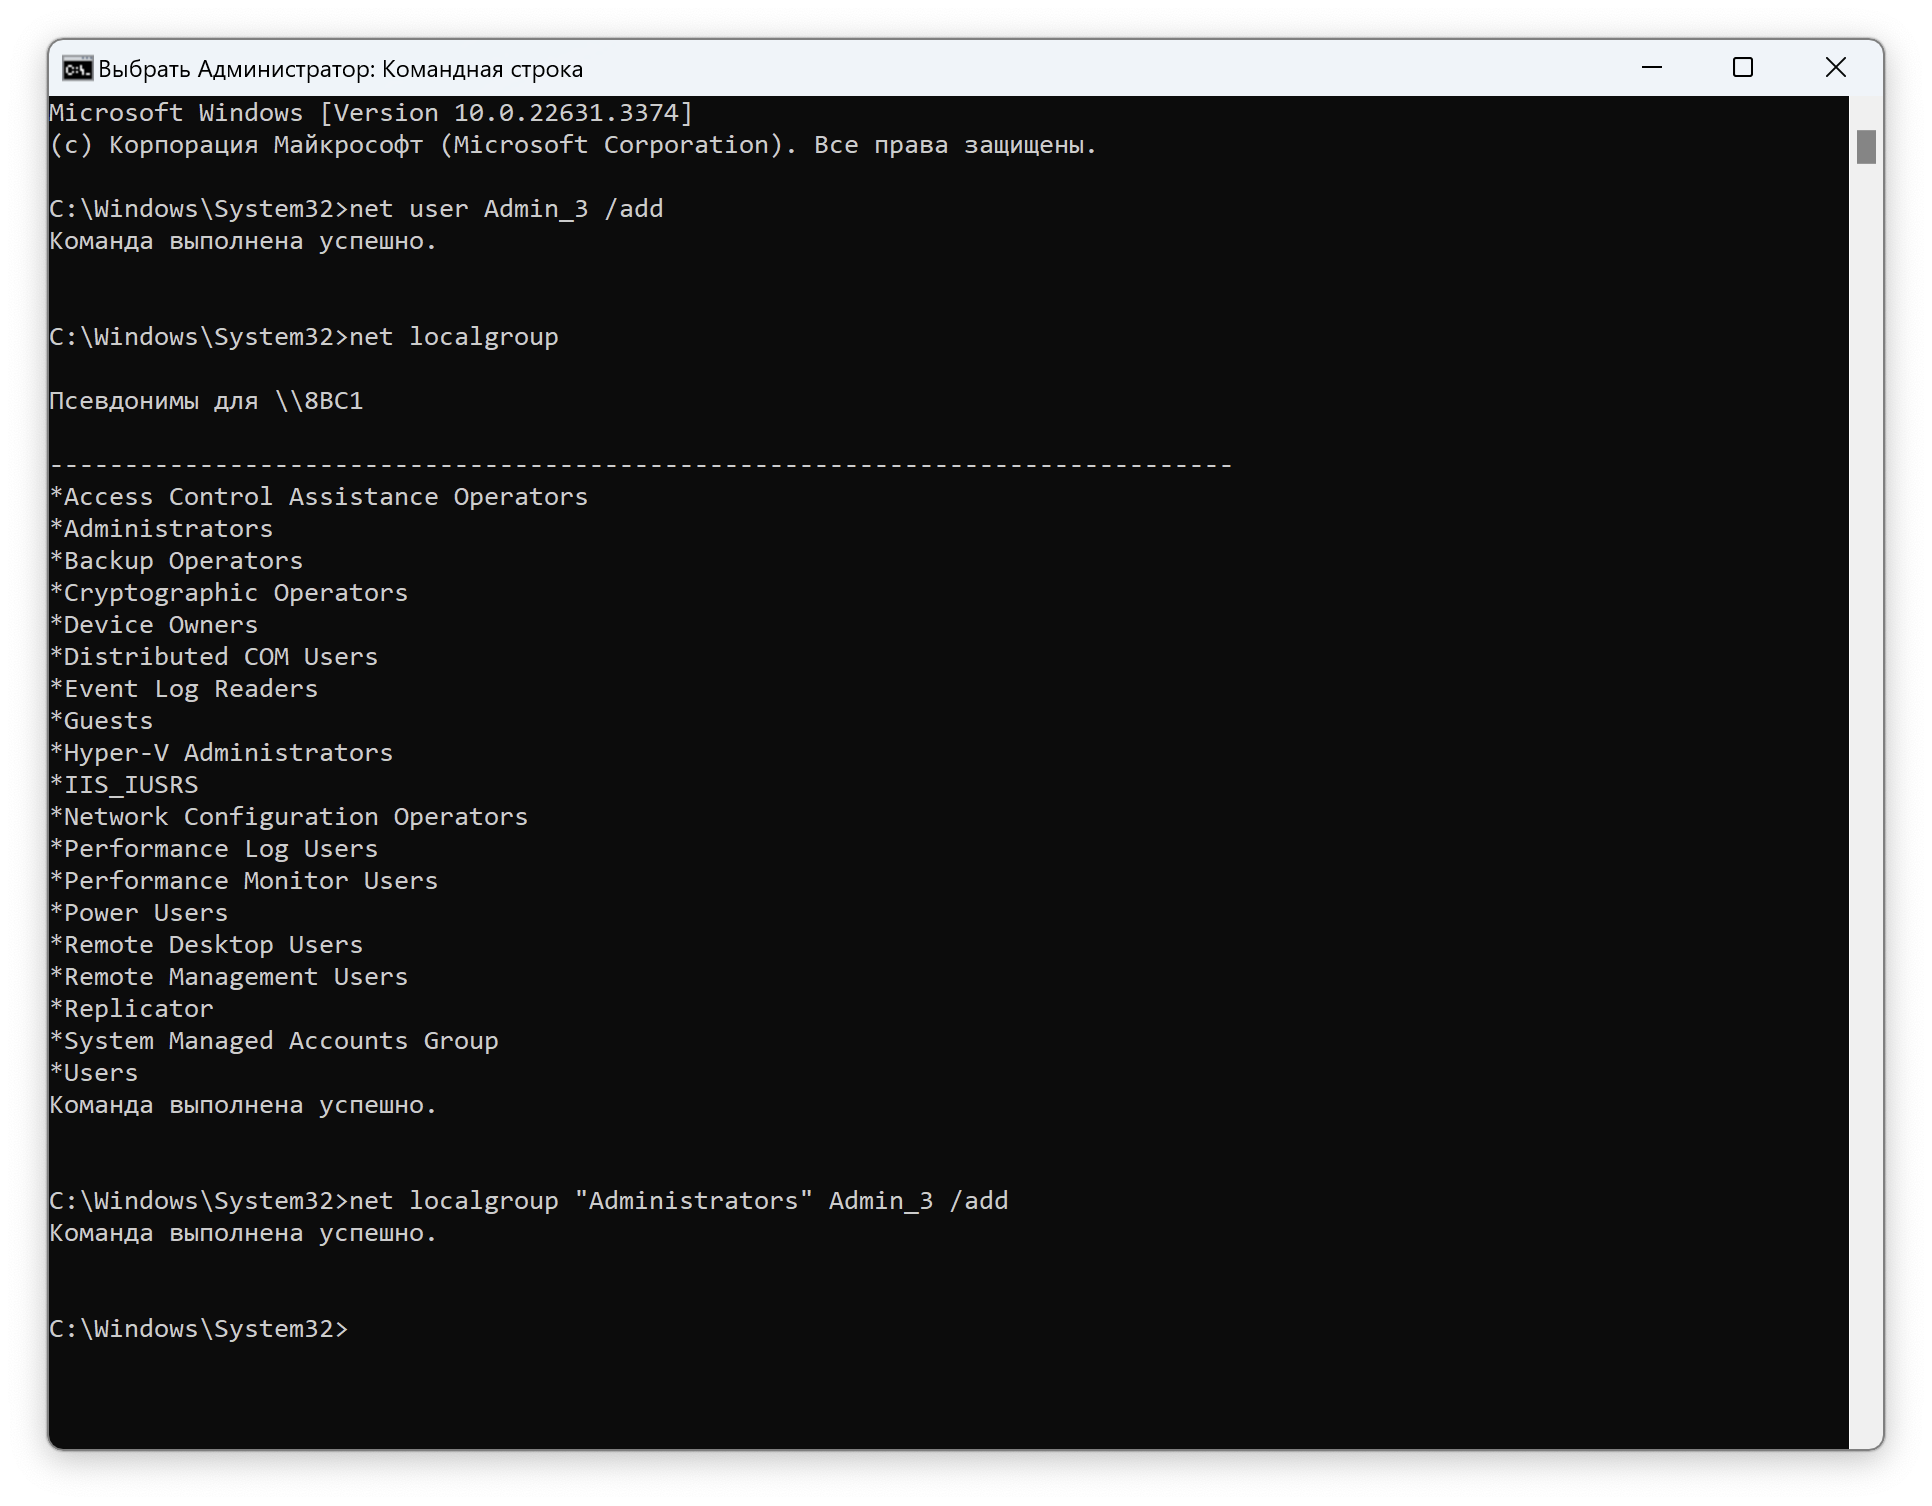
\includegraphics[width=0.8\textwidth]{../images/cmd_create_admin.png}
              \caption{Создание администратора с помощью командной строки}
          \end{figure}
          }
\end{enumerate}
% \nsubsection{Вариант 4. Создание администратора с помощью PowerShell}
% \begin{enumerate}
%     \item Откроем PowerShell от имени администратора.
%     \item Введем команду \texttt{New-LocalUser}
%     \item Введем имя пользователя и пароль.
%     \item Введем команду \texttt{Add-LocalGroupMember -Group "Administrators" -Member <имя пользователя>}
%     \item {
%           \begin{figure}[H]
%               \centering
%               \includegraphics[width=0.8\textwidth]{../images/powershell_create_admin.png}
%               \caption{Создание администратора с помощью PowerShell}
%           \end{figure}
%           }
% \end{enumerate}
\nsubsection{Ограничения администратора по конфигурации системы}
\begin{enumerate}
    \item Администратор может не может удалять некоторые системные приложения.
          \begin{figure}[H]
              \centering
              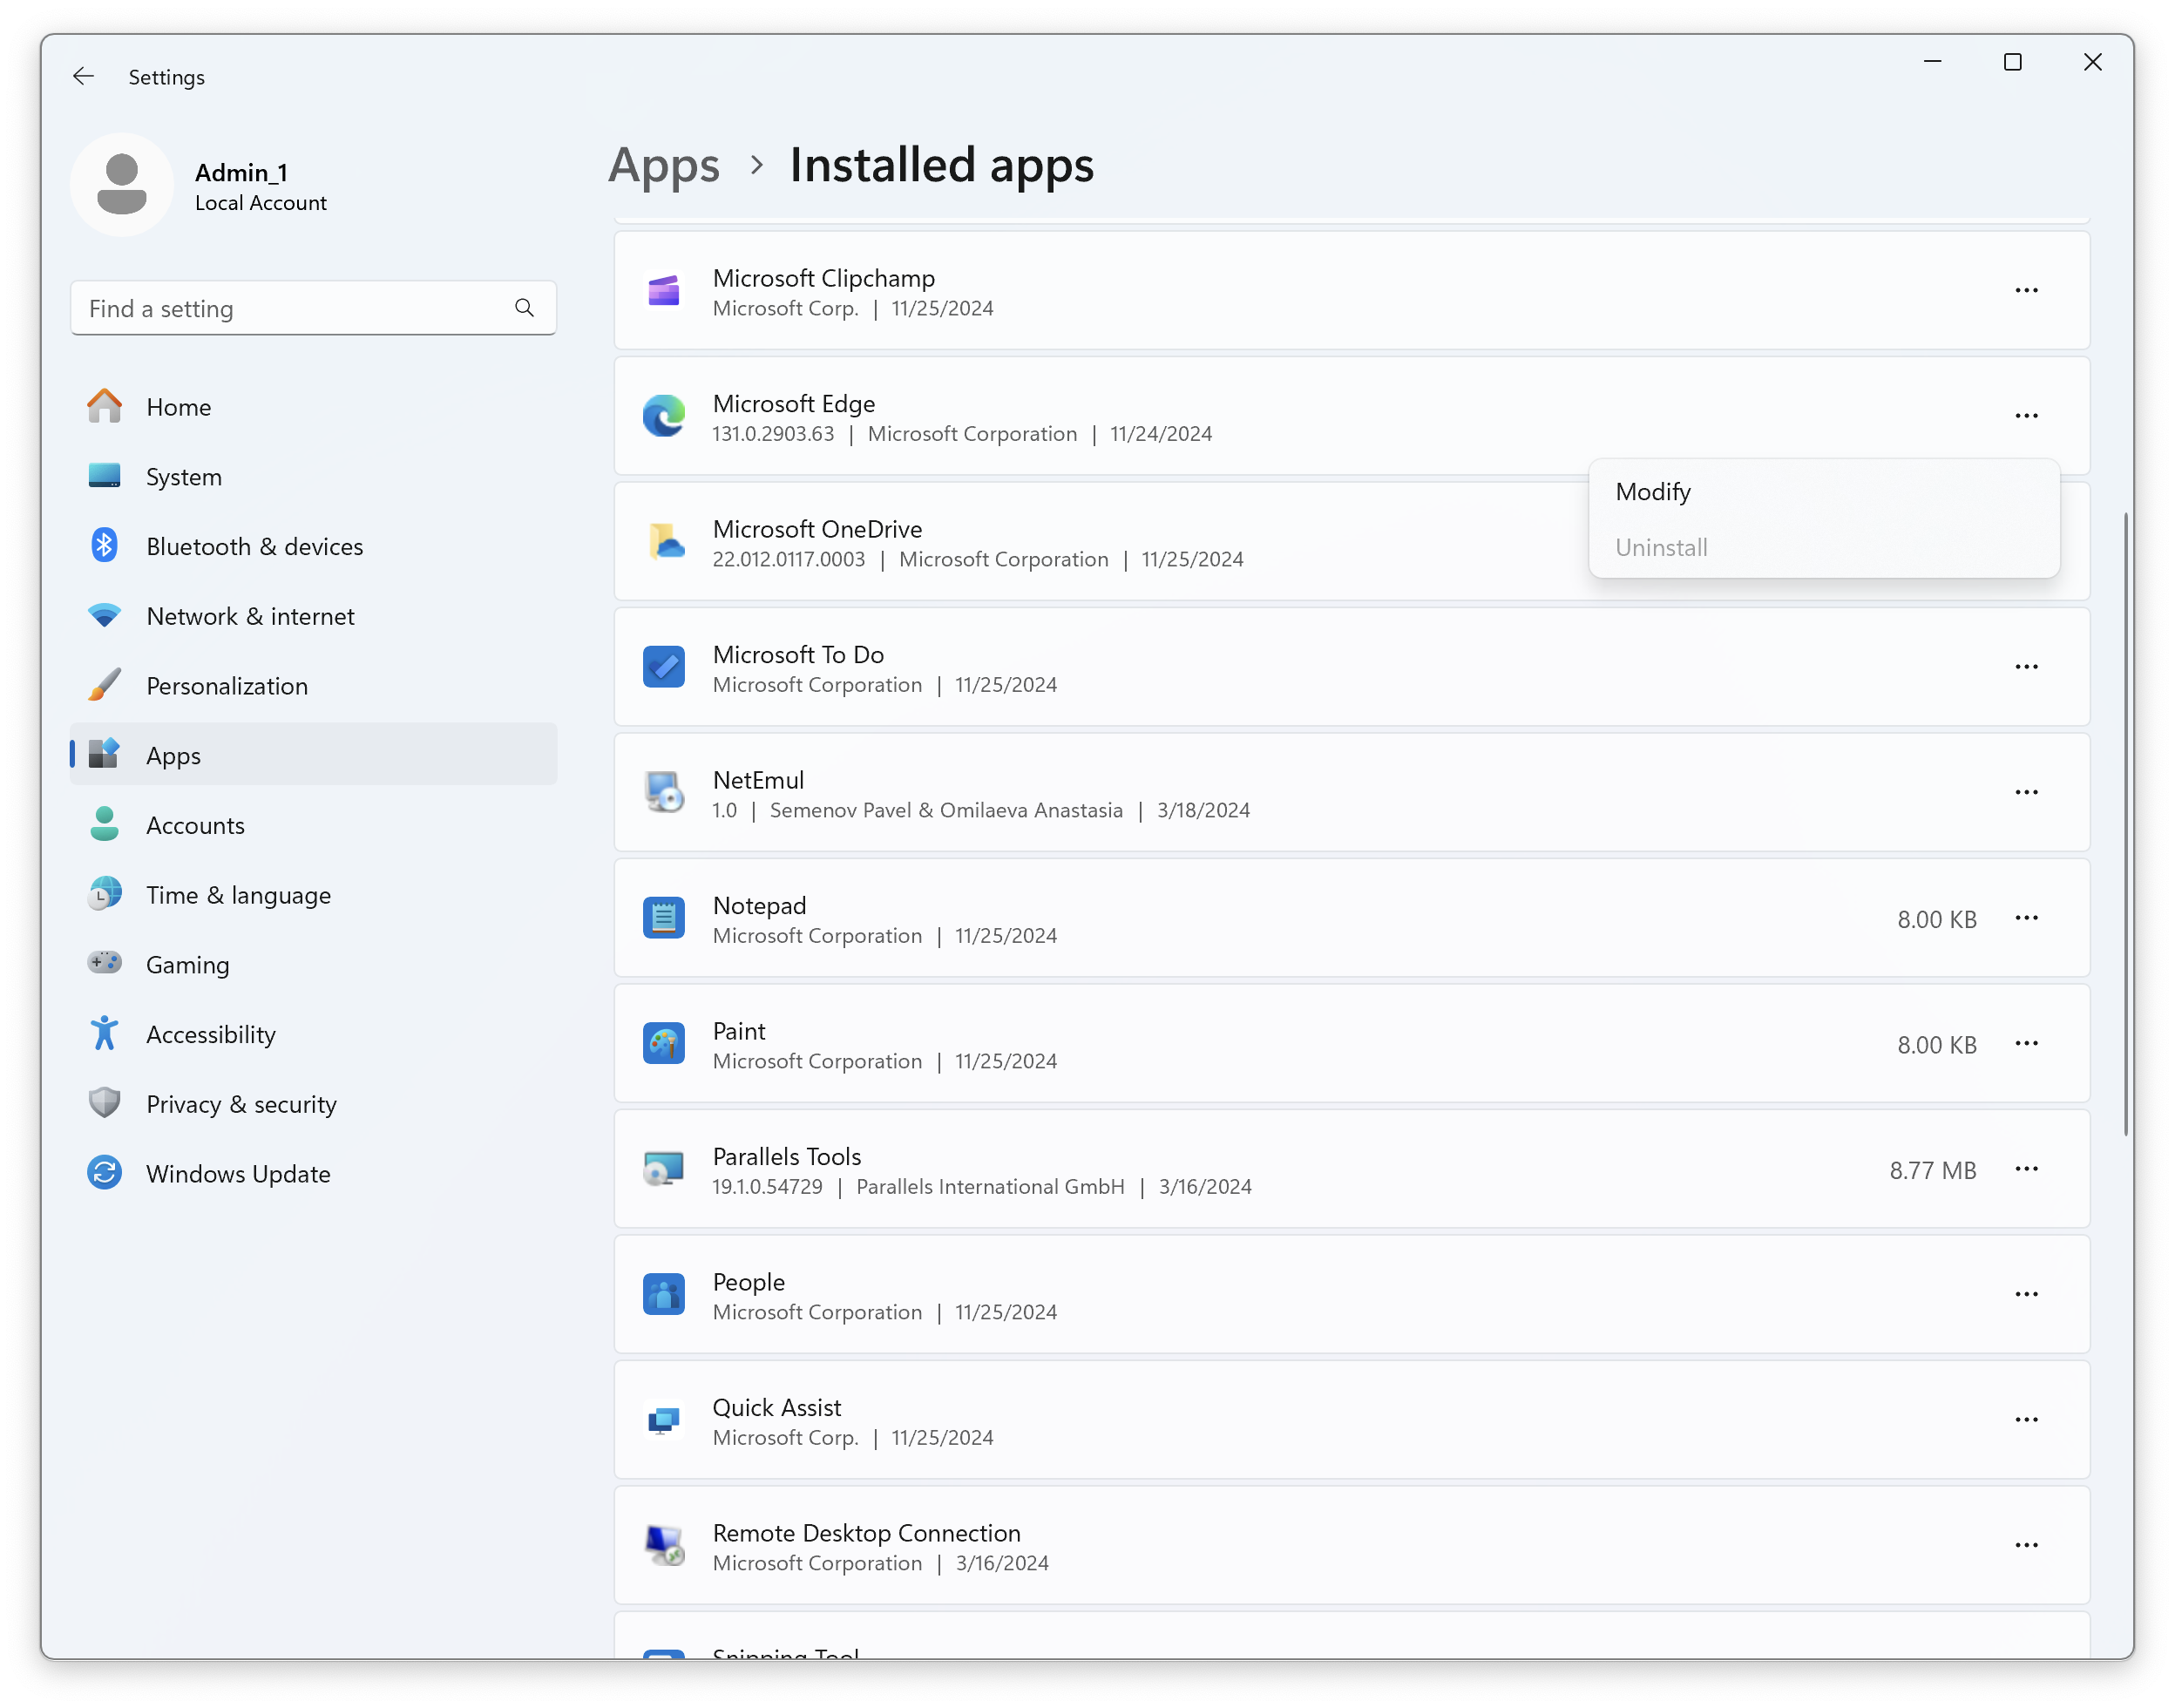
\includegraphics[width=0.8\textwidth]{../images/remove_system_apps.png}
              \caption{Удаление «важного» системного приложения}
          \end{figure}
    \item Администратор не может удалять встроенные группы. К примеру, группу «Guests».
          \begin{figure}[H]
              \centering
              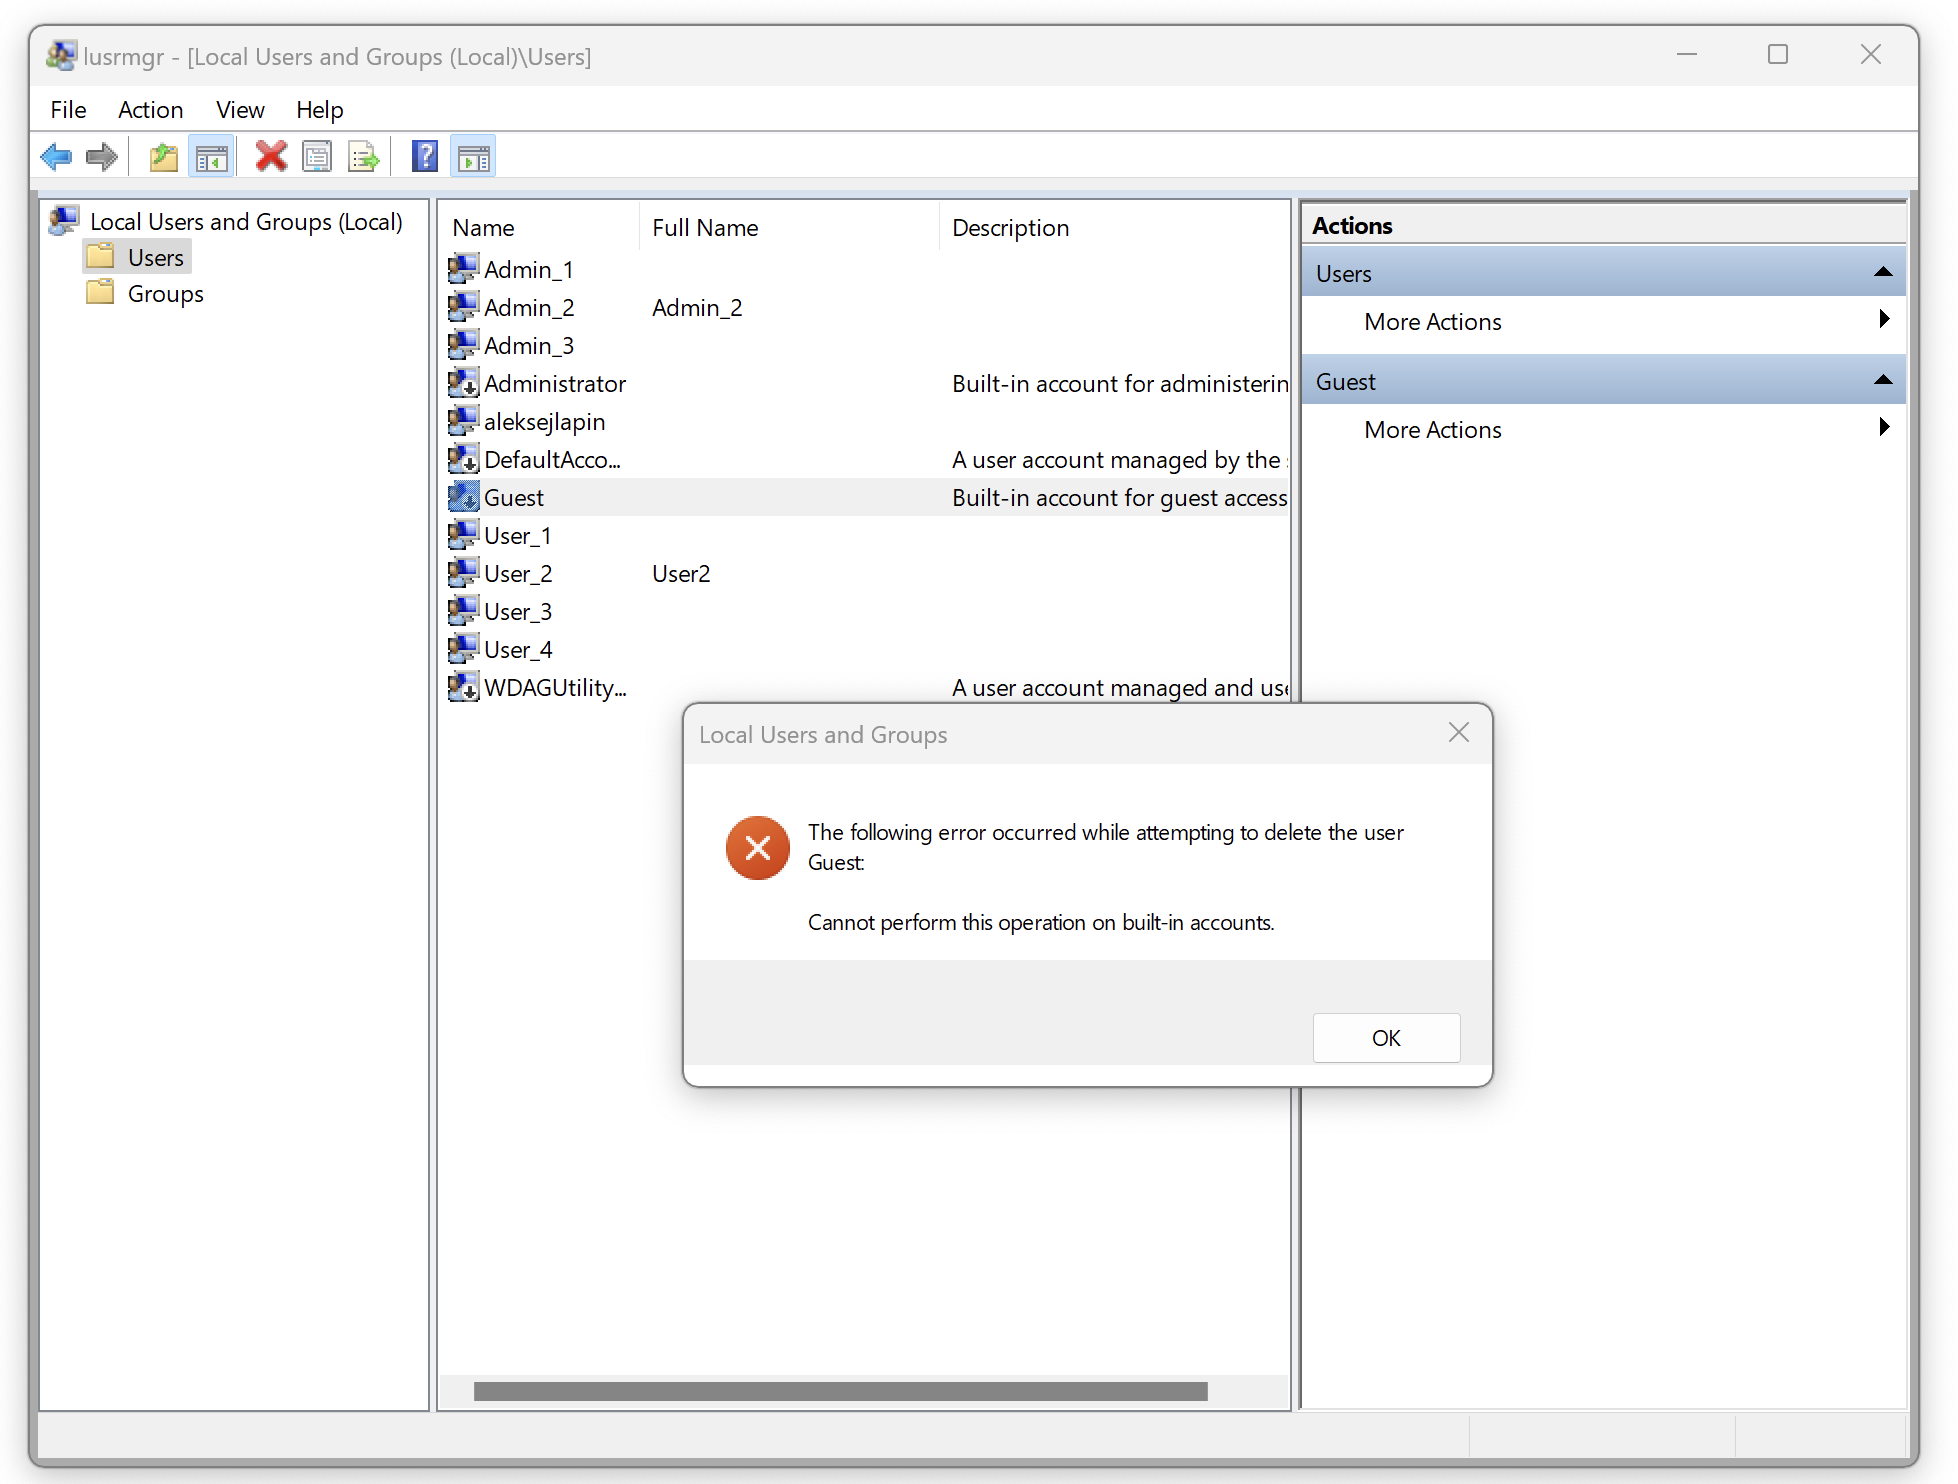
\includegraphics[width=0.8\textwidth]{../images/remove_builtin_group.png}
              \caption{Удаление встроенной группы}
          \end{figure}
    \item Администратор не может получить доступ к важным системным папкам.
          \begin{figure}[H]
              \centering
              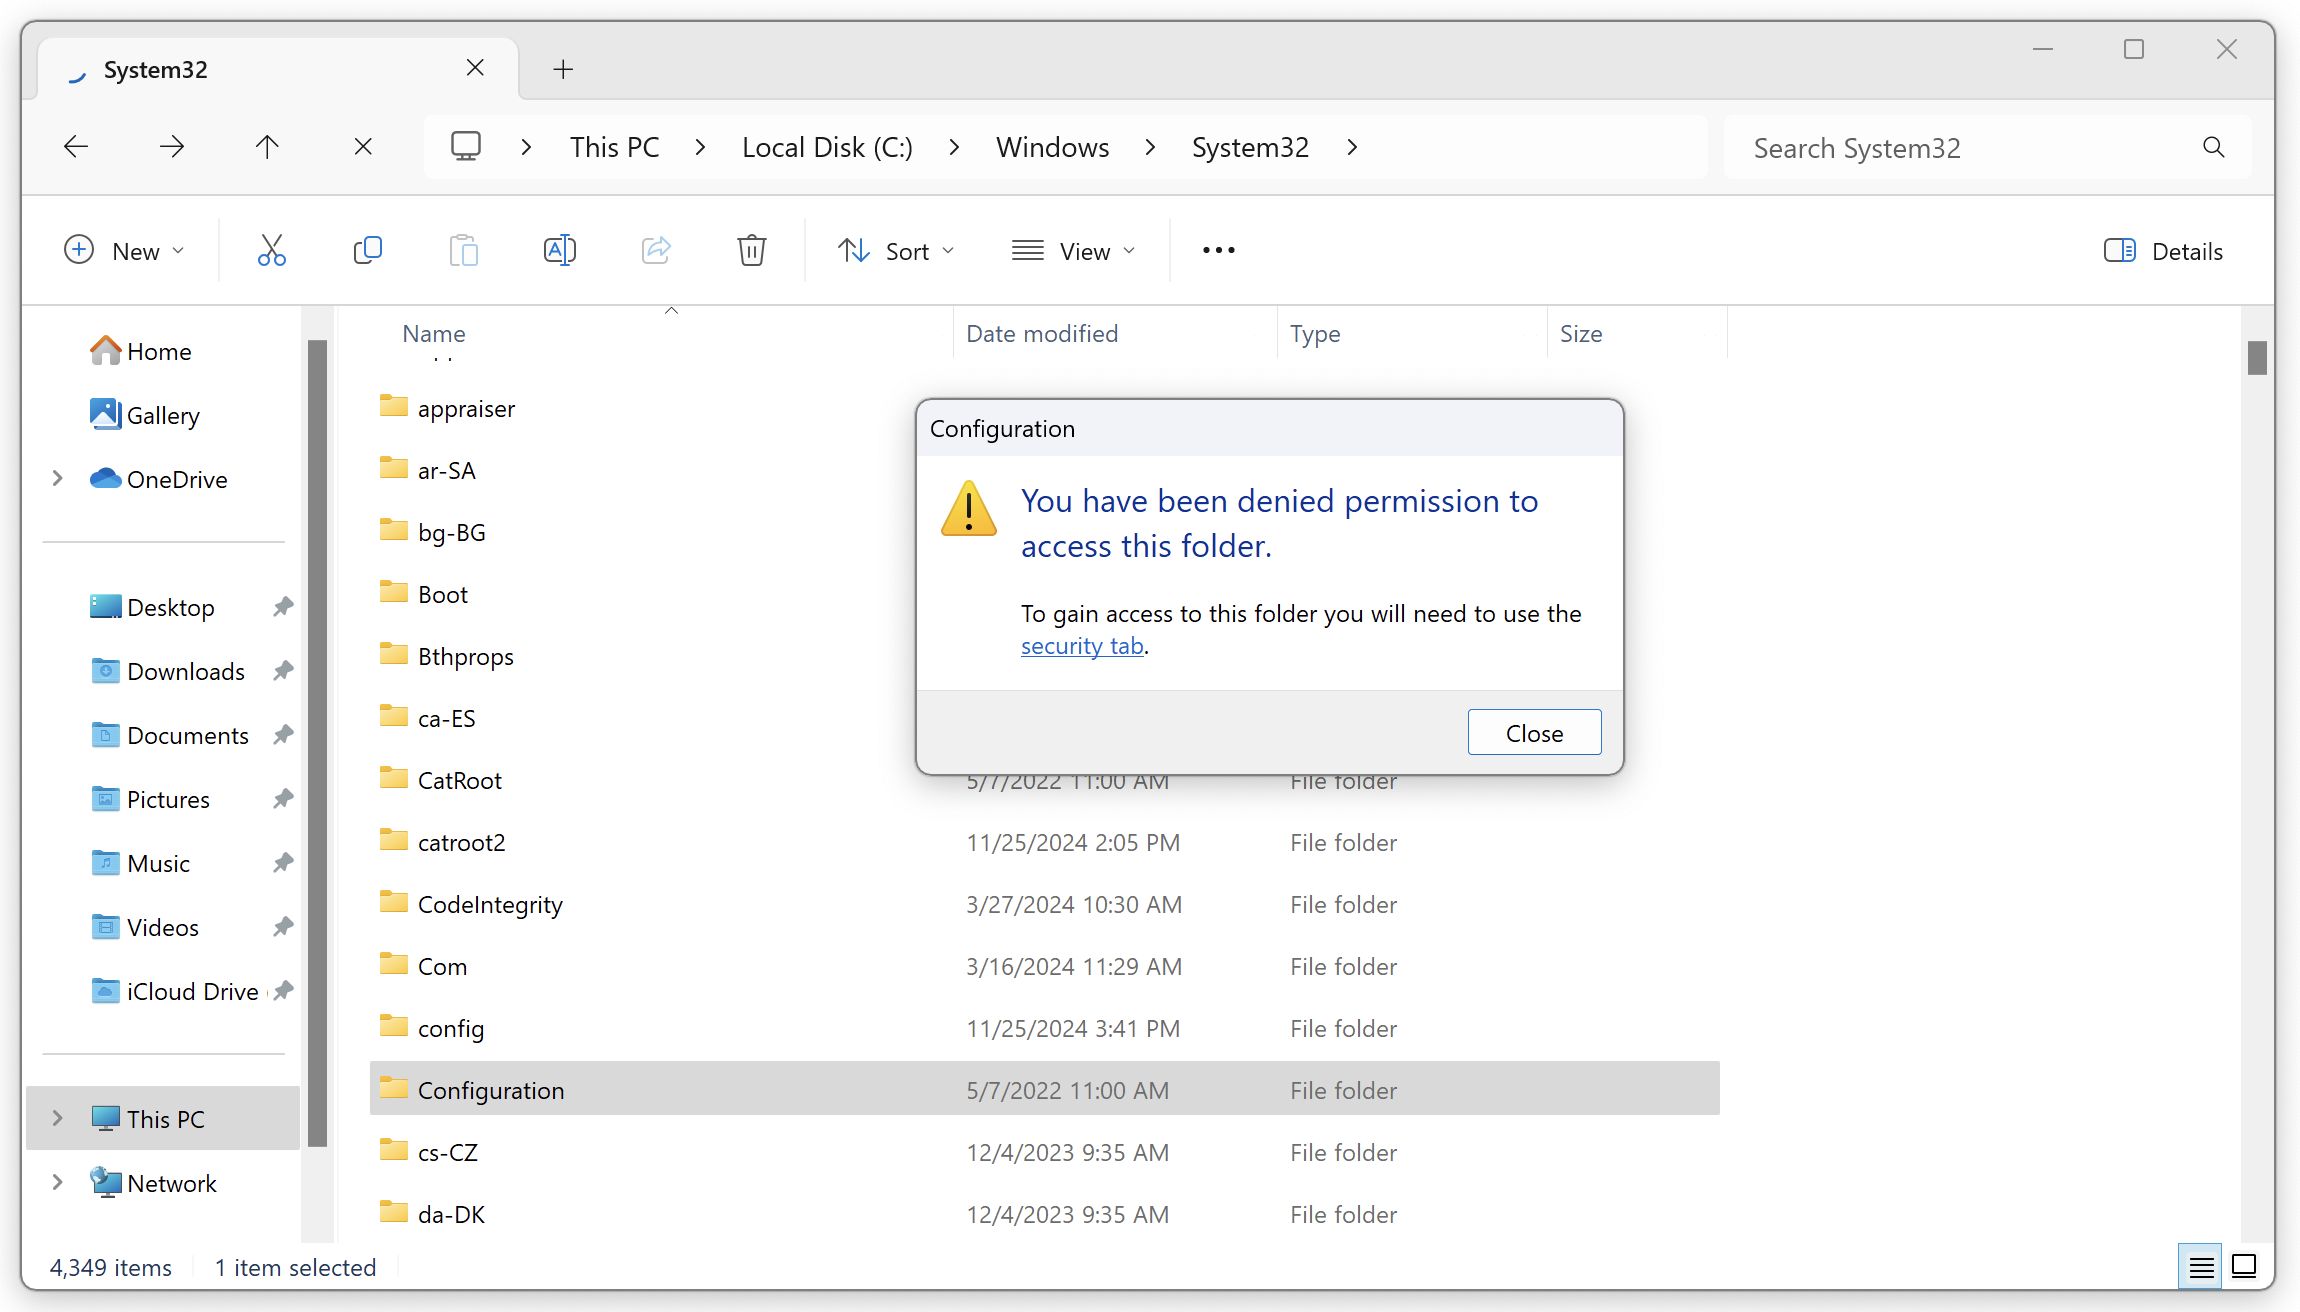
\includegraphics[width=0.8\textwidth]{../images/access_system_folders.png}
              \caption{Доступ к важной системной папке}
          \end{figure}
    \item Администратор не может изменять параметры автозапуска некоторых служб.
          \begin{figure}[H]
              \centering
              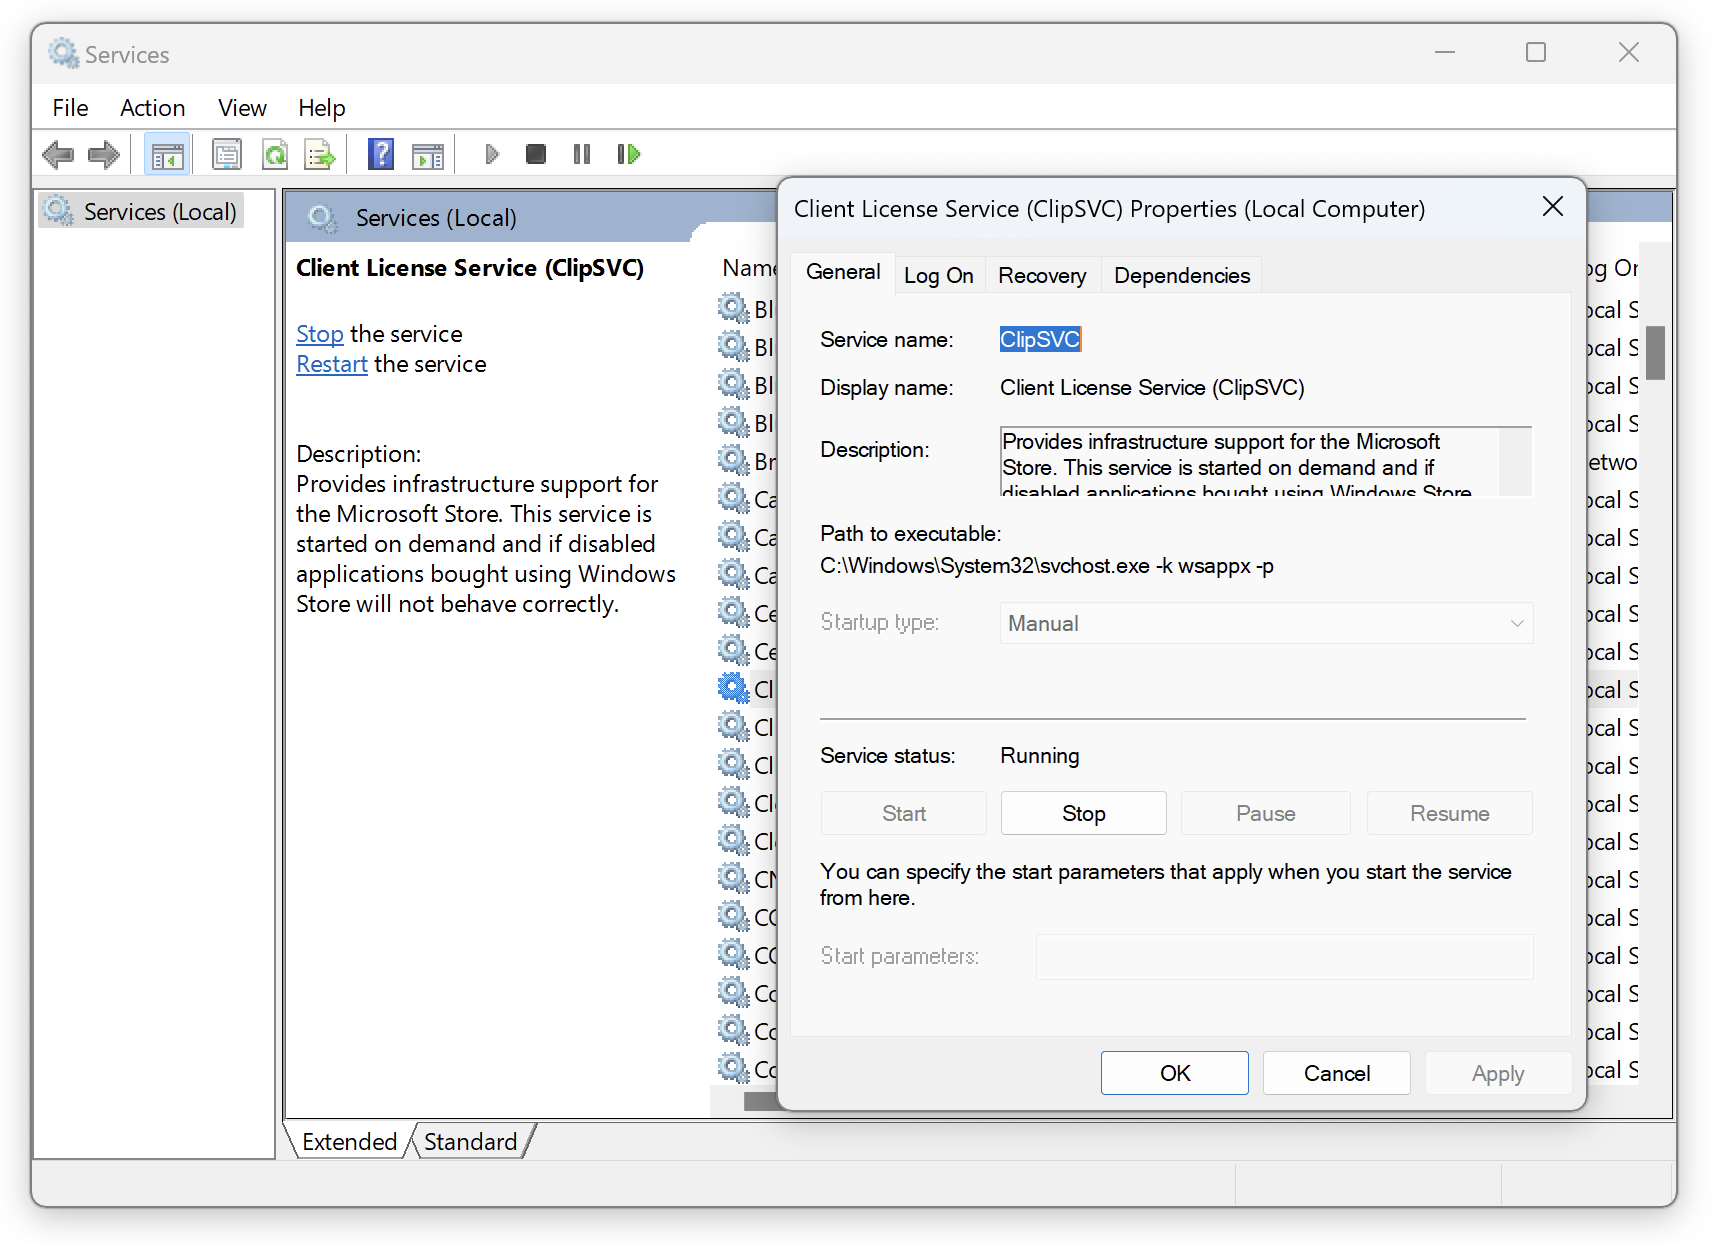
\includegraphics[width=0.8\textwidth]{../images/startup_client_license.png}
              \caption{Изменение параметров автозапуска службы Client License Service}
          \end{figure}
          \begin{figure}[H]
              \centering
              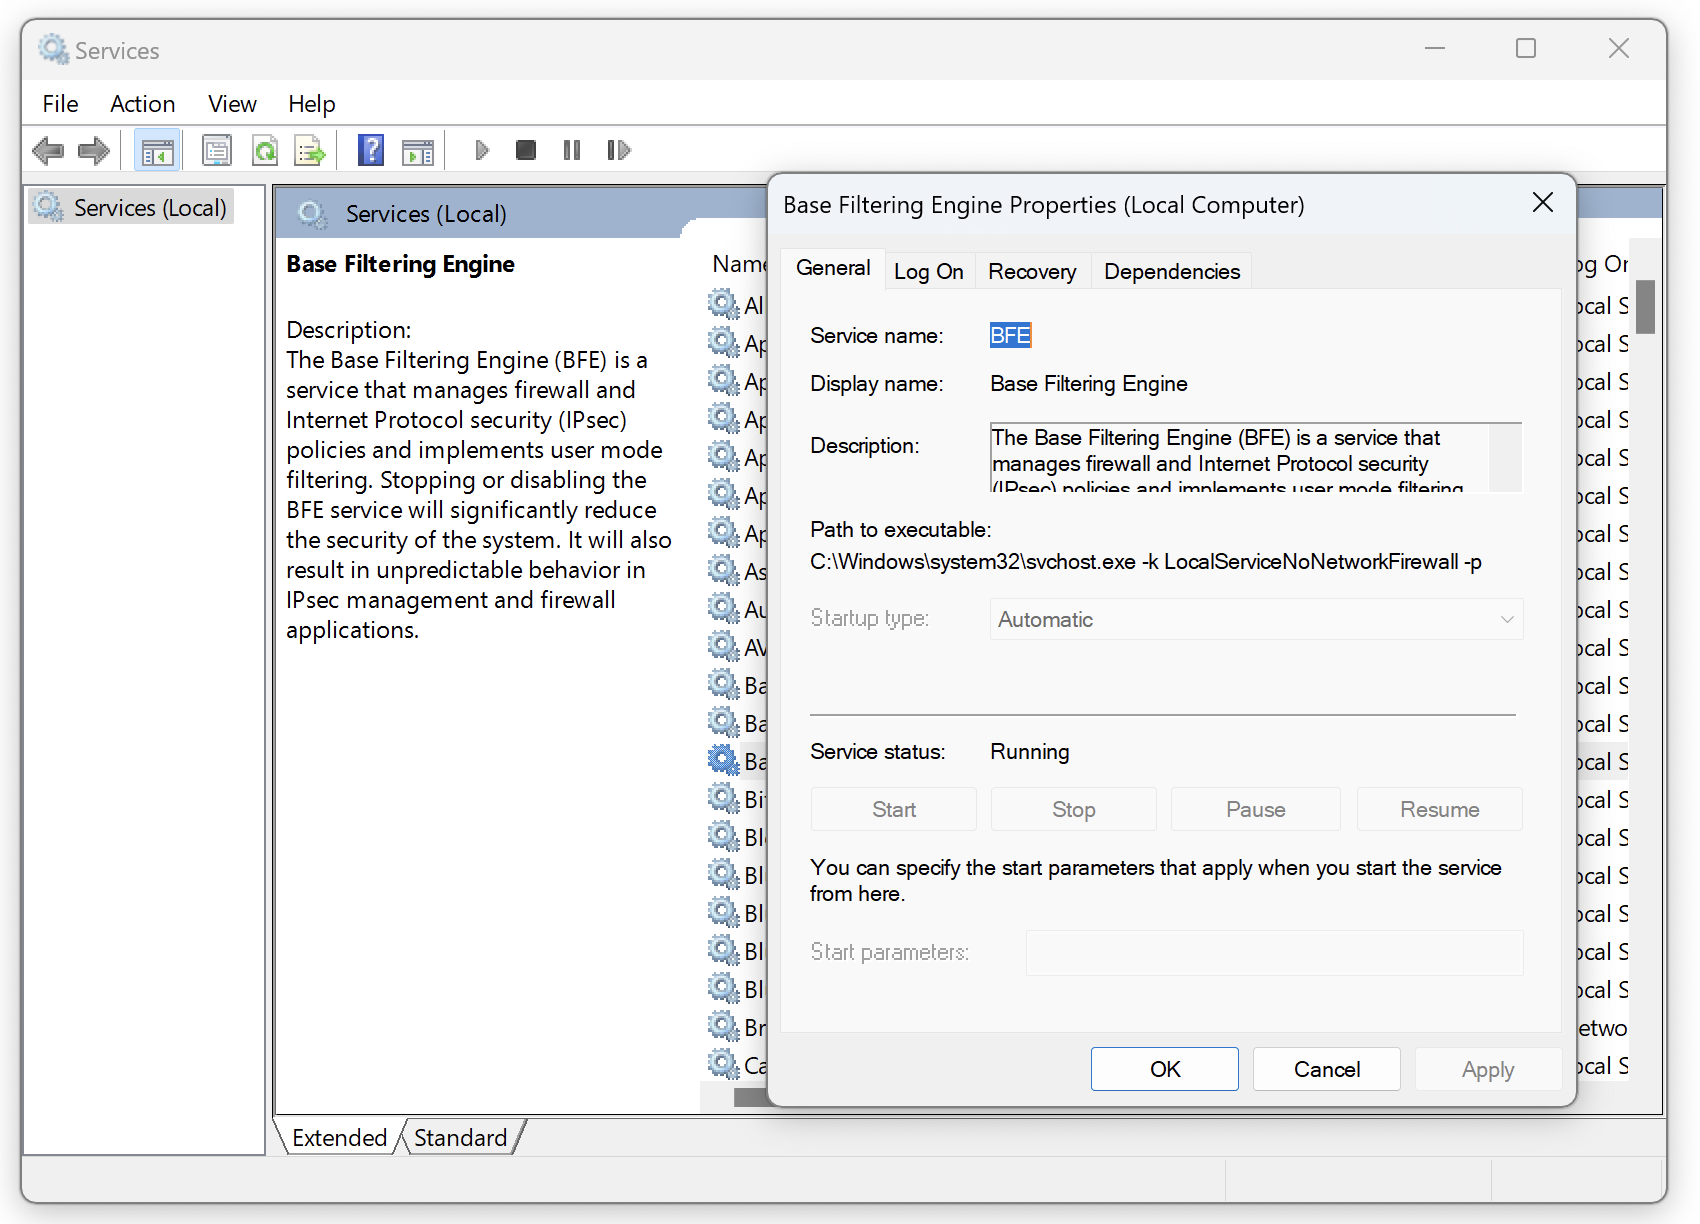
\includegraphics[width=0.8\textwidth]{../images/startup_bfe.png}
              \caption{Изменение параметров автозапуска службы Base Filtering Engine}
          \end{figure}
\end{enumerate}
\section{Параметры контроля учетных записей пользователей (UAC)}
UAC (User Account Control или контроль учетных записей) важный компонент системы защиты Windows. При запуске любого приложения или процесса, который требует прав администратора, пытается изменить системные настройки, ветки реестра или файлы, компонент контроля учетных записей UAC переключает рабочий стол в защищенный режим и запрашивает подтверждение этих действий у администратора. Тем самым UAC позволяет предотвратить запуск процессов и вредоносных программ, которые потенциально могут нанести вред вашему компьютеру.

\nsubsection{Ползунок User Account Control}

В Windows 7 (и выше) настройки UAC на компьютере управляются с помощью специального ползунка (вызывается через панель управления или файлом UserAccountControlSettings.exe ).
С помощью ползунка вы можете выбрать один из четырех предопределенных уровней защиты UAC.
\begin{itemize}
    \item {Всегда уведомлять в следующих случаях
          \begin{itemize}
              \item Когда приложения пытаются установить
                    программное обеспечение или изменить
                    параметры компьютера
              \item Когда я изменяю параметры Windows
          \end{itemize}
          \textcolor{blue}{\faInfoCircle} Рекомендуется при частой установке нового
          программного обеспечения и посещении
          незнакомых веб-сайтов.
          }
    \item {Уведомлять только при попытках приложений внести изменения в компьютер (по умолчанию)
          \begin{itemize}
              \item Не уведомлять при изменении параметров Windows пользователем
          \end{itemize}
          \textcolor{blue}{\faInfoCircle} Рекомендуется при использовании знакомых
          приложений и посещении знакомых веб-сайтов.
          }
    \item Уведомлять только при попытках приложений
          внести изменения в компьютер (не затемнять
          рабочий стол)
          {\begin{itemize}
                      \item Не уведомлять, когда я изменяю параметры Windows
                  \end{itemize}
              }
          \textcolor{blue}{\faInfoCircle} Не рекомендуется. Выбирайте этот вариант,
          только если затемнение рабочего стола
          компьютера занимает много времени.
    \item {Не уведомлять меня:
          \begin{itemize}
              \item Когда приложения пытаются установить
                    программное обеспечение или изменить
                    параметры компьютера
              \item Когда я изменяю параметры Windows
          \end{itemize}
          \textcolor{blue}{\faInfoCircle} Не рекомендуется.          }
\end{itemize}

По умолчанию в Windows 11 выбран 3 уровень защиты UAC, который выводит уведомление только при попытке изменить системные файлы или параметры.
\begin{figure}[H]
    \centering
    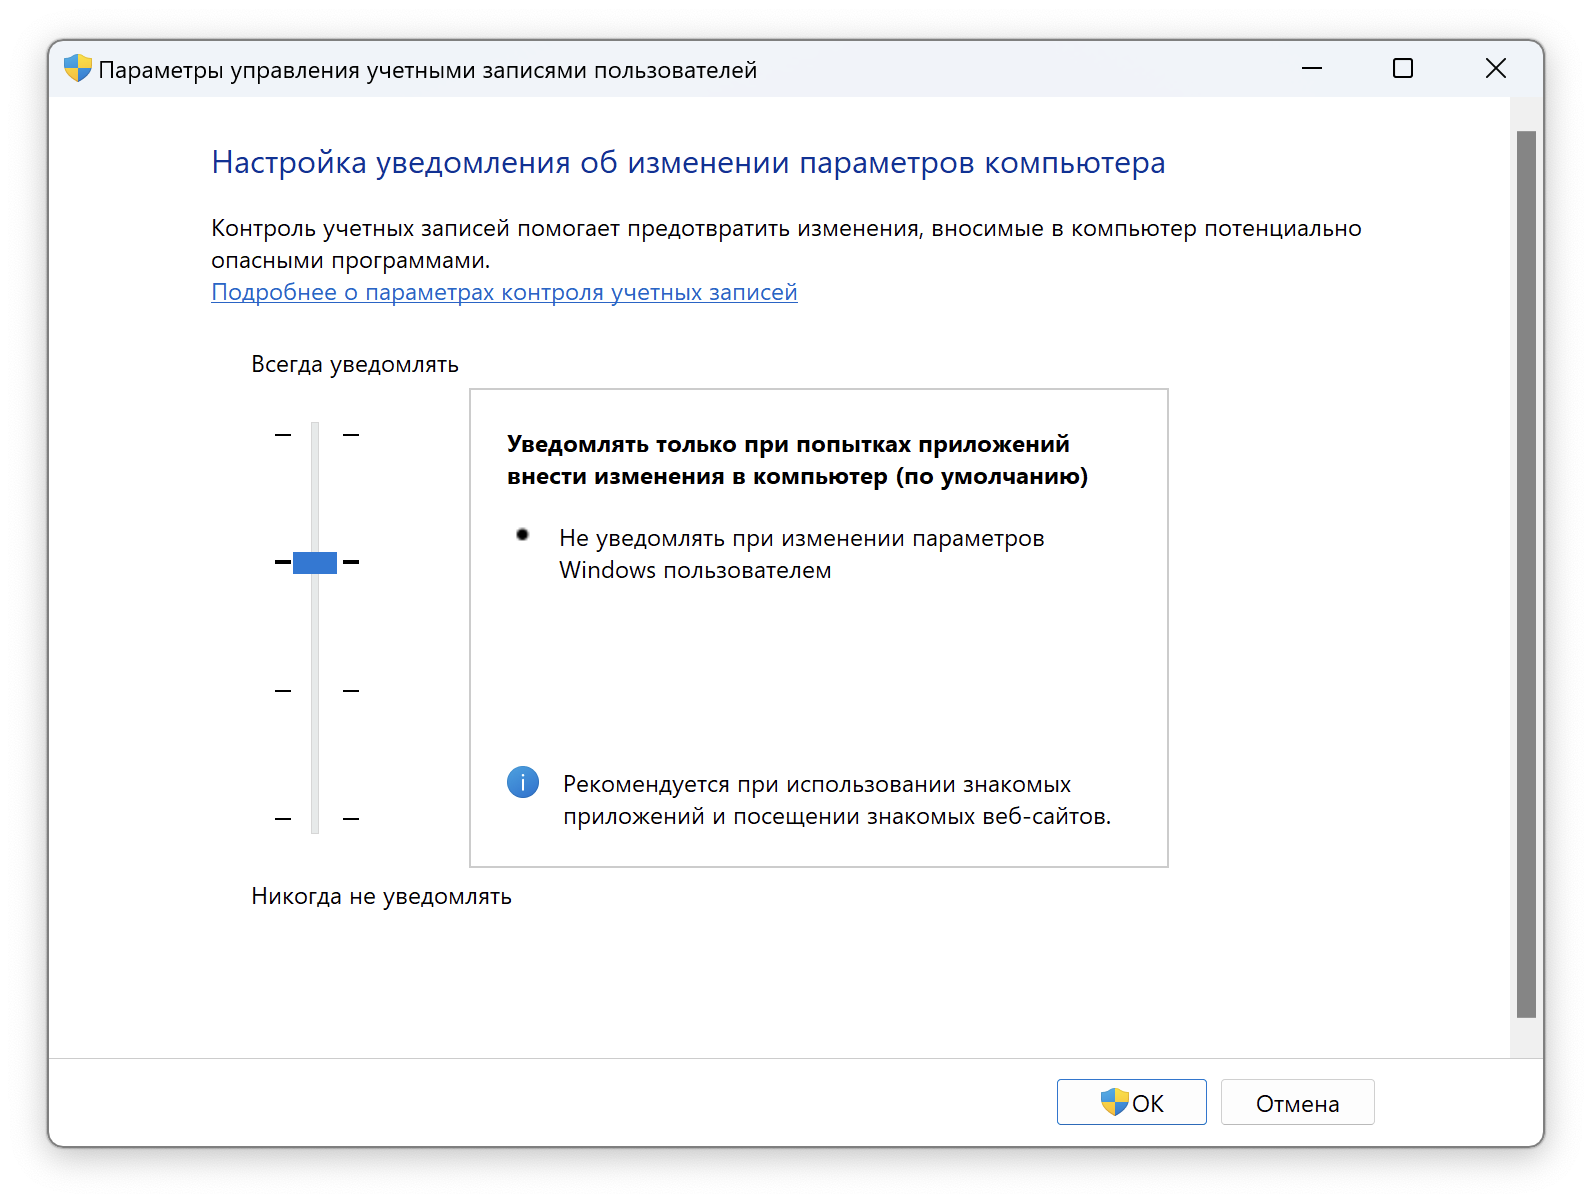
\includegraphics[width=0.8\textwidth]{../images/uac_level.png}
    \caption{Уровень защиты UAC}
\end{figure}

\section{Выполнить настройки механизмов защиты ОС Windows в соответствии с вариантом}
\begin{tcolorbox}[colback=white!95!gray, colframe=black, title=Вариант 1]
    Настроить вход пользователя в систему по паролю.

    Рассмотреть и реализовать возможные способы усиления парольной защиты.
\end{tcolorbox}
В процессе создания пользователей был установлен пароль для входа в систему.
По умолчанию нет ограничений по сложности пароля.
\begin{figure}[H]
    \centering
    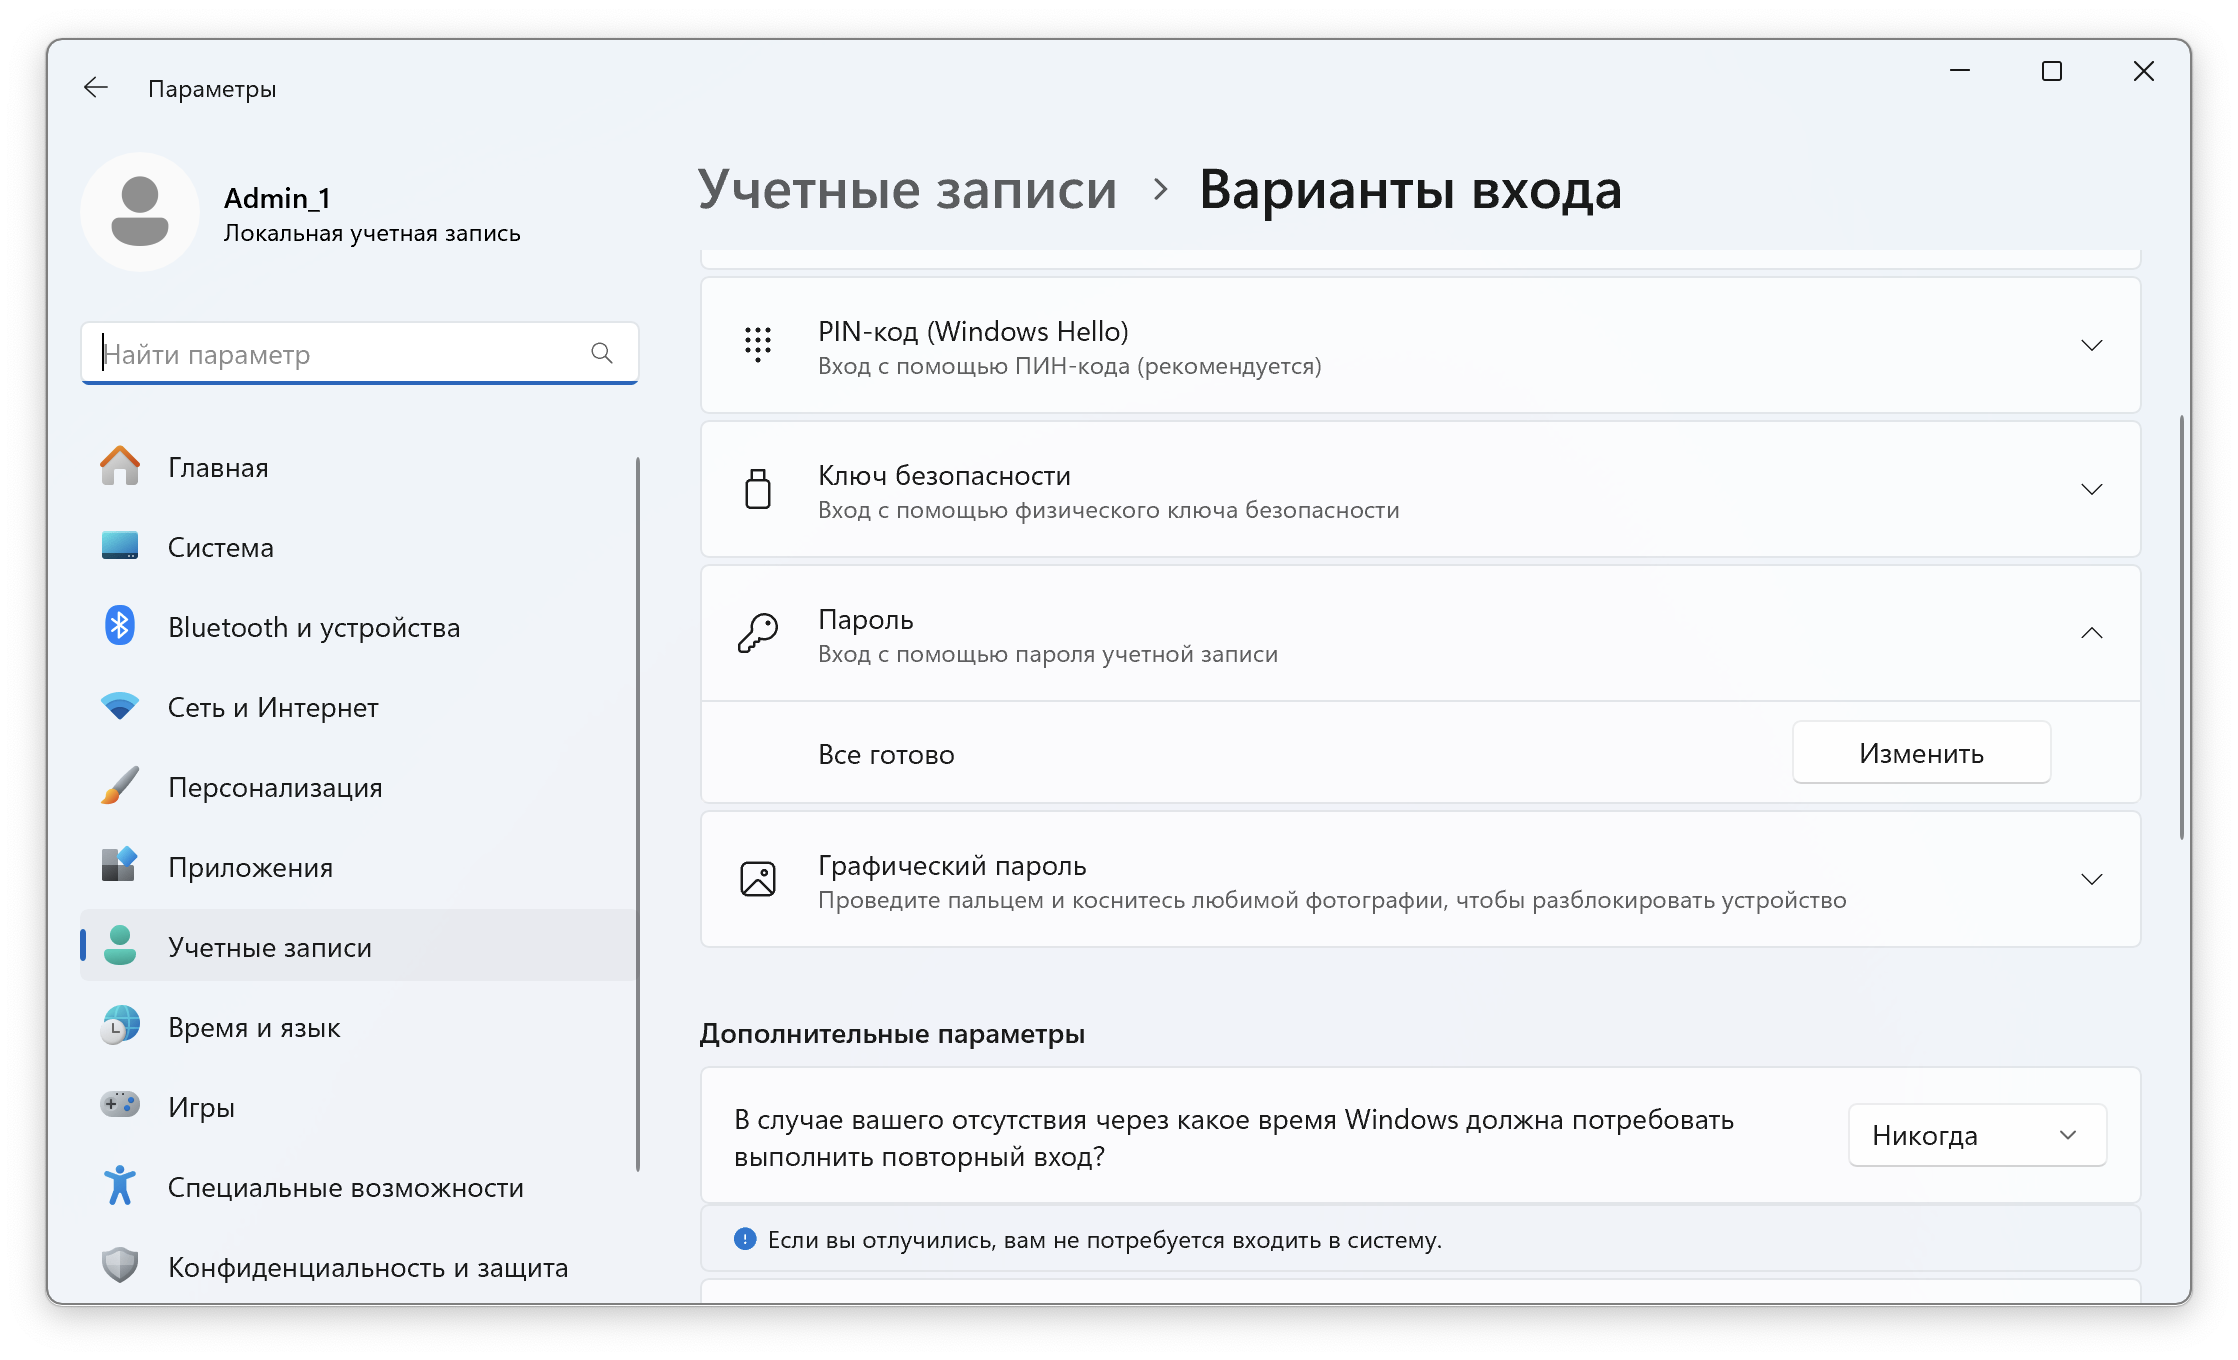
\includegraphics[width=0.8\textwidth]{../images/password_settings.png}
    \caption{Пароль пользователя}
\end{figure}
\nsubsection{Меры по усилению парольной защиты.}
Для усиления парольной защиты в Windows 11 можно использовать групповые политики безопасности:

\begin{enumerate}
    \item Открываем редактор локальной групповой политики с помощью команды \texttt{gpedit.msc}
    \item Переходим в раздел \texttt{Конфигурация компьютера > Конфигурация Windows > Параметры безопасности > Политики учетных записей > Политика паролей}
    \item Можем настроить следующие параметры:
          \begin{itemize}
              \item Аудит минимальной длины пароля
                    \begin{itemize}
                        \item Позволяет отслеживать попытки создания паролей короче минимальной длины
                        \item События записываются в журнал безопасности Windows
                        \item Помогает выявить пользователей, пытающихся обойти политику безопасности
                    \end{itemize}
              \item Вести журнал паролей
                    \begin{itemize}
                        \item Хранит историю использованных паролей
                        \item Предотвращает повторное использование старых паролей
                        \item Повышает безопасность, заставляя создавать новые пароли
                    \end{itemize}
              \item Максимальный срок действия пароля
                    \begin{itemize}
                        \item Определяет период, после которого пароль должен быть изменен
                        \item Снижает риск компрометации при длительном использовании одного пароля
                        \item Рекомендуется устанавливать 60-90 дней
                    \end{itemize}
              \item Минимальная длина пароля
                    \begin{itemize}
                        \item Задает минимальное количество символов в пароле
                        \item Длинные пароли сложнее подобрать
                        \item Рекомендуется минимум 8-12 символов
                    \end{itemize}
              \item Минимальный срок действия пароля
                    \begin{itemize}
                        \item Определяет период, в течение которого нельзя изменить пароль
                        \item Предотвращает немедленную смену пароля обратно на старый
                        \item Усиливает эффективность журнала паролей
                    \end{itemize}
              \item Ослабить ограничение минимальной длины пароля
                    \begin{itemize}
                        \item Позволяет создавать пароли короче установленной минимальной длины
                        \item Не рекомендуется включать
                        \item Используется только в особых случаях для совместимости
                    \end{itemize}
              \item Пароль должен отвечать требованиям сложности
                    \begin{itemize}
                        \item Требует использования разных типов символов
                        \item Увеличивает энтропию пароля
                        \item Делает пароль более устойчивым к подбору
                    \end{itemize}
              \item Хранить пароли, используя обратимое шифрование
                    \begin{itemize}
                        \item Позволяет восстановить исходный пароль
                        \item Снижает безопасность системы
                        \item Включается только если требуется протоколами или приложениями
                    \end{itemize}
          \end{itemize}
          \begin{figure}[H]
              \centering
              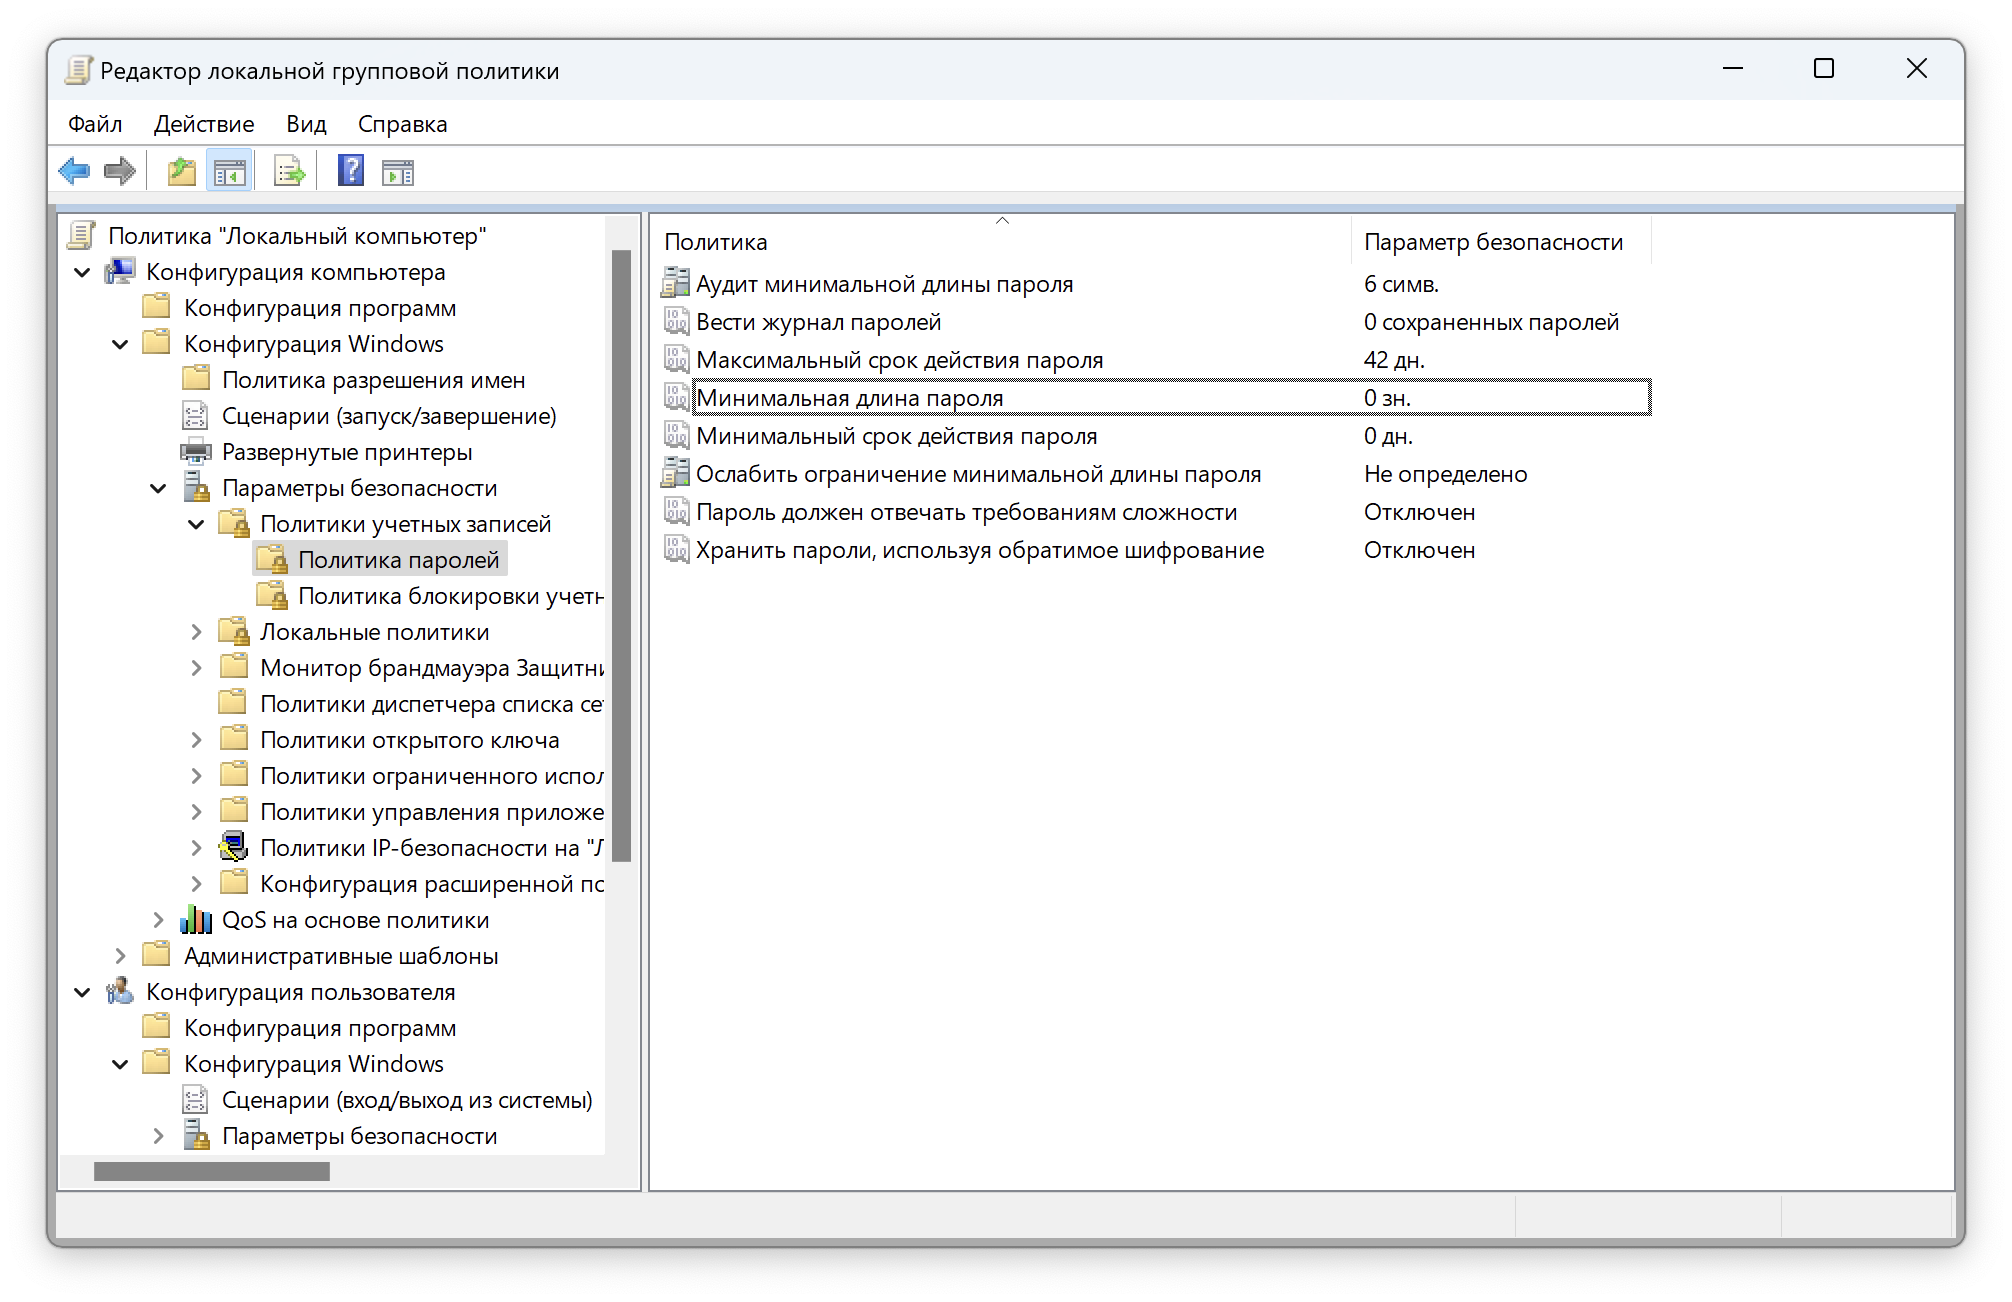
\includegraphics[width=0.8\textwidth]{../images/password_policy.png}
              \caption{Политика паролей}
          \end{figure}
\end{enumerate}

\nsubsection{Меры по усилению парольной защиты с помощью политик блокировки учетной записи в Windows 11}
\begin{enumerate}
    \item \textbf{Настройка политики блокировки учетных записей:}
          \begin{itemize}
              \item Откройте редактор локальной групповой политики, введя команду \texttt{gpedit.msc} в диалоговом окне "Выполнить" (Win + R).
              \item Перейдите в раздел \texttt{Конфигурация компьютера > Параметры Windows > Параметры безопасности > Политики учетных записей > Политика блокировки учетных записей}.
          \end{itemize}
    \item \textbf{Параметры политики блокировки и их назначение:}
          \begin{itemize}
              \item \textbf{Время до сброса счетчика блокировки:}
                    \begin{itemize}
                        \item Определяет время в минутах до обнуления счетчика неудачных попыток входа
                        \item Предотвращает атаки перебором, растянутые во времени
                        \item Позволяет легитимным пользователям повторить попытку входа после периода ожидания
                    \end{itemize}
              \item \textbf{Пороговое значение блокировки:}
                    \begin{itemize}
                        \item Задает количество неудачных попыток входа до блокировки учетной записи
                        \item Защищает от автоматизированного подбора паролей
                        \item Предотвращает атаки методом "грубой силы"
                    \end{itemize}
              \item \textbf{Продолжительность блокировки учетной записи:}
                    \begin{itemize}
                        \item Устанавливает время, на которое блокируется учетная запись
                        \item Предотвращает немедленные повторные попытки взлома
                        \item Дает время администраторам для реагирования на подозрительную активность
                    \end{itemize}
              \item \textbf{Разрешить блокировку учетной записи администратора:}
                    \begin{itemize}
                        \item Определяет, применяются ли правила блокировки к учетной записи администратора
                        \item Повышает безопасность, но может создать риск полной блокировки системы
                        \item Требует наличия резервной административной учетной записи
                    \end{itemize}
          \end{itemize}
          \begin{figure}[H]
              \centering
              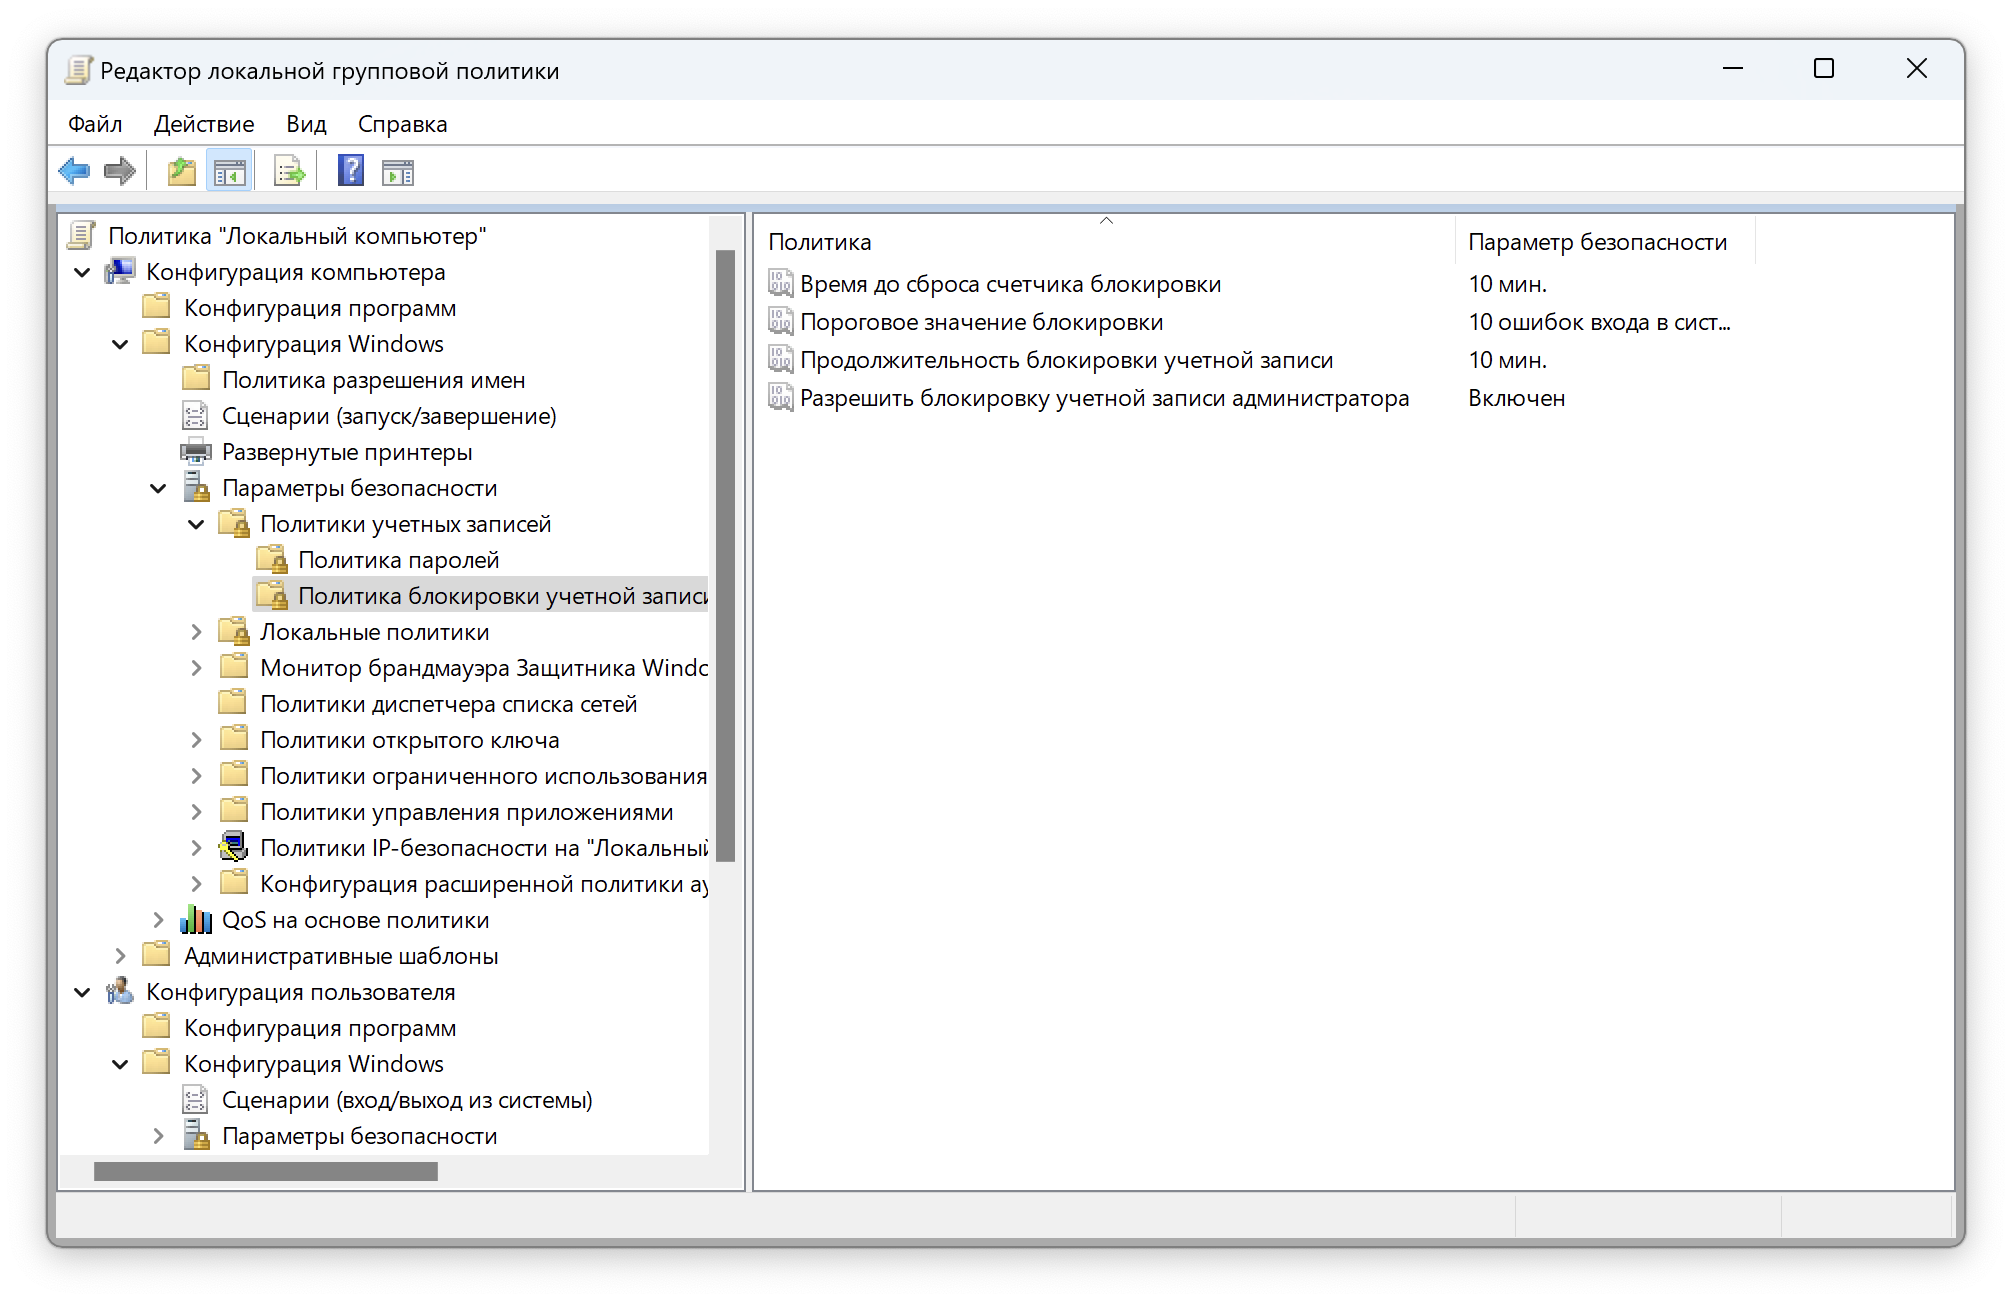
\includegraphics[width=0.8\textwidth]{../images/account_lockout_policy.png}
              \caption{Политика блокировки учетных записей}
          \end{figure}
\end{enumerate}
\nsubsection{Меры по усилению парольной защиты с помощью команды Net Accounts}
Команда Net Accounts используется для задания параметров политики на локальном компьютере, таких как политики учетных записей и политики паролей.
\begin{enumerate}
    \item Откроем командную строку от имени администратора.
    \item Введем команду \texttt{net accounts}
    \item Вы увидите параметры политики блокировки учетных записей по умолчанию и политики паролей на локальном компьютере, как показано ниже.
          \begin{figure}[H]
              \centering
              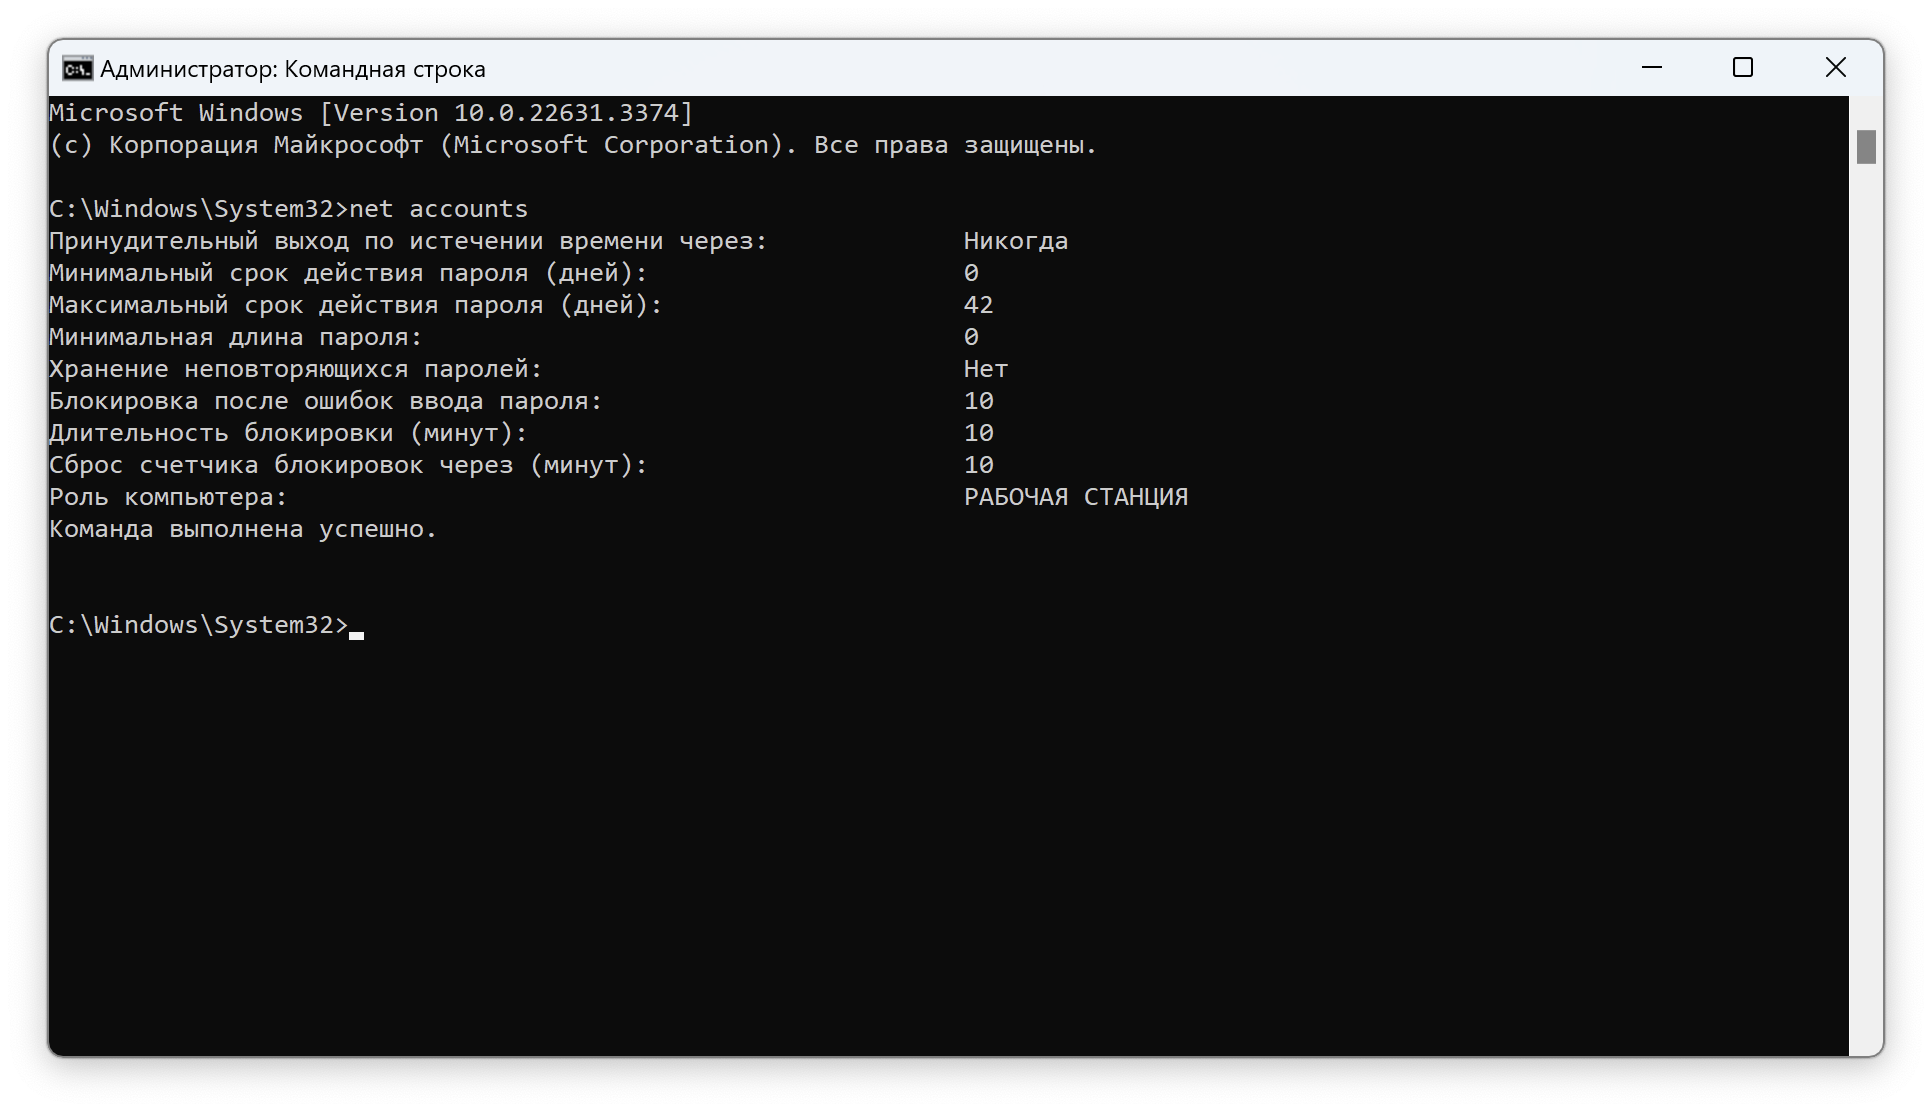
\includegraphics[width=0.8\textwidth]{../images/net_accounts.png}
              \caption{Параметры политики блокировки учетных записей и паролей}
          \end{figure}
    \item Приведенные выше параметры отображаются в качестве роли компьютера. Если компьютер присоединен к домену, параметры домена вступают в силу, и будут отображаться только параметры, поступающие из домена. Остальные параметры будут локальными параметрами, если он не поступает из объекта групповой политики домена.

    \item Вы можете изменить следующие параметры в параметрах Net Accounts:
          \begin{itemize}
              \item \textbf{\texttt{/FORCELOGOFF:{minutes | NO}}}: Задает количество минут, когда срок действия учетной записи истекает или истекает срок действия допустимого срока входа. Нет, значение по умолчанию предотвращает принудительный выход.
              \item \textbf{\texttt{/MINPWLEN:length}}: Задает минимальное количество символов для пароля. Диапазон равен 0–14 символам; Значение по умолчанию — шесть символов.
              \item \textbf{\texttt{/MAXPWAGE:{days | UNLIMITED}}}: Задает максимальное количество дней, в течение которых пароль действителен. Ограничение не указано с помощью \texttt{UNLIMITED}. Значение \texttt{/MAXPWAGE} не может быть меньше \texttt{/MINPWAGE}. Диапазон равен 1–999; Значение по умолчанию — 90 дней.
              \item \textbf{\texttt{/MINPWAGE:days}}: Задает минимальное количество дней, которые должны пройти, прежде чем пользователь сможет изменить пароль. Значение нуля не задает минимальное время. Диапазон равен 0–999; значение по умолчанию равно нулю дням. \texttt{/MINPWAGE} не может быть больше \texttt{/MAXPWAGE}.
              \item \textbf{\texttt{/UNIQUEPW:number}}: Задает количество уникальных паролей, которые должны быть использованы перед повторным использованием одного и того же пароля. Максимальное значение равно 24.
              \item \textbf{\texttt{/DOMAIN}}: Выполняет операцию на контроллере домена текущего домена. В противном случае операция выполняется на локальном компьютере.
              \item \textbf{\texttt{net help accounts}}: Отображение справки для указанной команды net.
          \end{itemize}
          \begin{figure}[H]
              \centering
              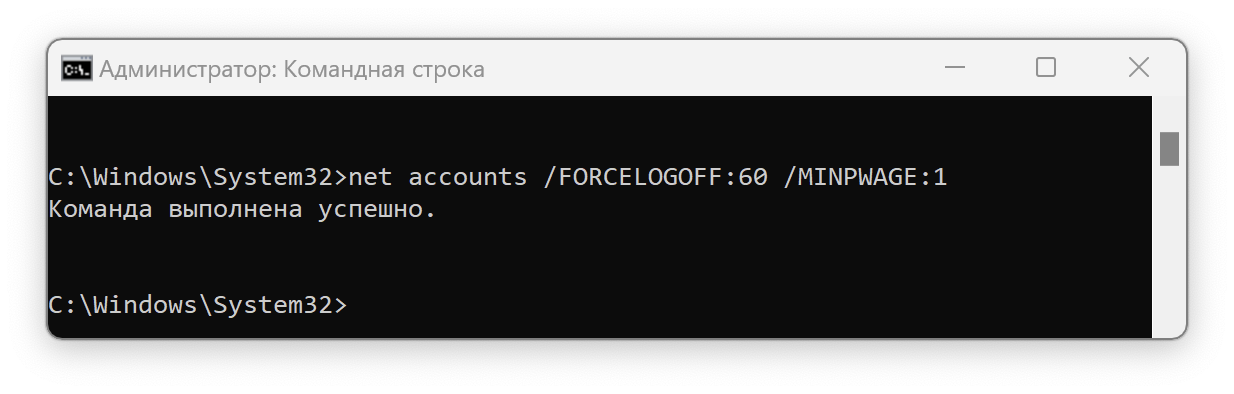
\includegraphics[width=0.8\textwidth]{../images/net_accounts_example.png}
              \caption{Пример команды Net Accounts}
          \end{figure}
\end{enumerate}
Мои действия по настройке механизма защиты, включающие установку пароля для пользователя, не соответствуют ряду требований, указанных в руководящих документах. В частности, они не удовлетворяют требованиям «Очистка памяти», «Дискреционный принцип контроля доступа» и «Руководство для пользователя». Это связано с тем, что функциональность, о которой идёт речь, относится непосредственно к операционной системе Windows 10. Настройка входа по паролю направлена на выполнение требований идентифик��ции и аутентификации.
\section{Анализ реализации механизма защиты в ОС Windows}
С апреля 2022 года ФСТЭК приостановил действие сертификатов на все программное обеспечение Microsoft (как и многих других иностранных вендоров).
До этого момента, последняя версия Windows, которая имела сертификат ФСТЭК, была Windows 10. Сертификат No4369, устанавливающий 6 уровень доверия к системе по документу
«Требования по безопасности 26 информации, устанавливающие уровни доверия к
средствам технической защиты информации и средствам обеспечения безопасности
информационных технологий» (ФСТЭК России, 2020). 6 это минимальный уровень доверия к системе.
Средства, соответствующие 6 уровню доверия, применяются в значимых объектах критической информационной инфраструктуры 3 категории, в государственных информационных системах 3 класса защищенности, в автоматизированных системах управления производственными и технологическими процессами 3 класса защищенности, в информационных системах персональных данных при необходимости обеспечения 3 и 4 уровня защищенности персональных данных.
Что говорит о том, что Windows 10 не может быть использован для большинства критических объектов, но подходит для использования на персональных компьютерах, без критических данных.

\subsection{Анализ соответствия механизма защиты ОС Windows 11 классу защищенности 1Г}
В соответствии с положениями руководящего документа «Руководящий документ. Автоматизированные системы. Защита от несанкционированного доступа к информации. Классификация автоматизированных систем и требования по защите информации.», операционная система Windows 11 относится к классу систем 1Г.
\subsubsection{Соответствие подсистемы управления доступом}

\begin{enumerate}
    \item \textbf{Идентификация и проверка подлинности субъектов доступа:}
          \begin{itemize}
              \item Windows 11 поддерживает идентификацию пользователей через уникальные идентификаторы (логины) и пароли, соответствующие требованиям длины не менее шести буквенно-цифровых символов. Кроме того, поддерживаются многофакторная аутентификация (MFA) для усиления безопасности.
          \end{itemize}
    \item \textbf{Идентификация терминалов, ЭВМ и других объектов по логическим именам:}
          \begin{itemize}
              \item В Windows 11 каждый терминал и устройство в сети могут быть идентифицированы по уникальным именам (например, NetBIOS или DNS имена), что соответствует требованиям класса 1Г.
          \end{itemize}
    \item \textbf{Идентификация программ и файлов по именам:}
          \begin{itemize}
              \item Операционная система обеспечивает идентификацию программ, томов, каталогов, файлов и других объектов по их именам через файловую систему NTFS и механизмы разрешений.
          \end{itemize}
    \item \textbf{Контроль доступа в соответствии с матрицей доступа:}
          \begin{itemize}
              \item Windows 11 использует контроль доступа на основе списков контроля доступа (ACL), которые позволяют управлять правами доступа субъектов к различным ресурсам системы. Это позволяет реализовать матрицу доступа, определяющую права каждого пользователя.
          \end{itemize}
\end{enumerate}

\subsubsection{Соответствие подсистемы регистрации и учета}

\begin{enumerate}
    \item \textbf{Регистрация входа и выхода субъектов доступа:}
          \begin{itemize}
              \item Windows 11 ведет журналы безопасности (Security Logs) через журнал событий Windows, регистрируя успешные и неуспешные попытки входа пользователей, а также загрузку и останов системы.
          \end{itemize}
    \item \textbf{Регистрация выдачи печатных документов:}
          \begin{itemize}
              \item Система может регистрировать события печати через журналы событий, фиксируя дату, время, устройство вывода и пользователя, инициировавшего печать.
          \end{itemize}
    \item \textbf{Регистрация запуска и завершения программ и процессов:}
          \begin{itemize}
              \item Windows 11 регистрирует запуск и завершение процессов через журнал событий, включая информацию о времени, имени процесса и пользователе, инициировавшем действие.
          \end{itemize}
    \item \textbf{Регистрация попыток доступа к защищаемым файлам и объектам:}
          \begin{itemize}
              \item Система фиксирует попытки доступа к файлам и другим объектам в журнале безопасности, включая результат попытки, идентификатор пользователя и спецификацию объекта.
          \end{itemize}
    \item \textbf{Учет защищаемых носителей информации:}
          \begin{itemize}
              \item Windows 11 поддерживает шифрование данных на накопителях (BitLocker).
          \end{itemize}
    \item \textbf{Очистка освобождаемых областей памяти:}
          \begin{itemize}
              \item Операционная система обеспечивает базовую очистку оперативной памяти при закрытии процессов. Однако для выполнения требований класса 1Г, связанных с очисткой и перезаписью данных, могут потребоваться специализированные программные средства.
          \end{itemize}
\end{enumerate}

\subsubsection{Соответствие подсистемы обеспечения целостности}

\begin{enumerate}
    \item \textbf{Целостность программных средств СЗИ НСД:}
          \begin{itemize}
              \item Windows 11 использует цифровые подписи и проверки целостности системных файлов через механизмы защиты, такие как Windows Defender и механизмы Secure Boot, что способствует обеспечению целостности системных компонентов.
          \end{itemize}
    \item \textbf{Трансляция программной среды:}
          \begin{itemize}
              \item Использование современных компиляторов и защищенных сред разработки помогает поддерживать неизменность объектного кода программ при обработке и хранении защищаемой информации.
          \end{itemize}
    \item \textbf{Физическая охрана СВТ:}
          \begin{itemize}
              \item Физическая безопасность устройств и носителей информации зависит от инфраструктуры организации. Windows 11 предоставляет инструменты для управления доступом, но физическая охрана реализуется на уровне организации.
          \end{itemize}
    \item \textbf{Периодическое тестирование функций СЗИ НСД:}
          \begin{itemize}
              \item Windows 11 регулярно получает обновления безопасности и рекомендации по тестированию через Microsoft Security Compliance Toolkit. Однако организациям необходимо самостоятельно проводить тестирования с использованием специализированных тестовых программ.
          \end{itemize}
    \item \textbf{Средства восстановления СЗИ НСД:}
          \begin{itemize}
              \item Операционная система поддерживает функции восстановления и резервного копирования, однако для выполнения требований класса 1Г по ведению двух копий программных средств необходимо использовать дополнительные решения для резервного копирования и восстановления.
          \end{itemize}
    \item \textbf{Использование сертифицированных средств защиты:}
          \begin{itemize}
              \item Windows 11 сертифицирована по различным стандартам безопасности, включая FIPS 140-2 для криптографических модулей. Однако, для выполнения требований класса 1Г, связанных с использованием сертифицированных средств защиты, могут потребоваться специализированные программные средства сертифицированные ФСТЭК.
          \end{itemize}
\end{enumerate}

\subsubsection{Вывод}
Windows 11 обладает множеством встроенных функций безопасности, позволяющих удовлетворить основные требования класса защищенности 1Г,
такие как идентификация и аутентификация пользователей, контроль доступа, регистрация событий безопасности и обеспечение целостности системных компонентов.
Однако некоторые специфические требования класса 1Г, например, очистка с перезаписьюоперативной памяти,
требуют дополнительной настройки или использования специализированного программного обеспечения.
В целом, при правильной конфигурации и применении дополнительных мер, Windows 11 может соответствовать требованиям класса защищенности 1Г
для использования в менее критических информационных системах.
Отсутствие автоматической маркировки печатных документов и многократной очистки оперативной памяти и других требований не позволяет отнести Windows 11 к более высокому классу защищенности.
\subsection{Анализ соответствия защиты Windows 11 классу защищенности 6}
В соответствии с руководящим документом «Средства вычислительной техники. Защита от несанкционированного доступа к информации. Показатели защищенности от несанкционированного доступа к информации», Windows 11 относится к шестому классу защиты.

В данном разделе рассматривается соответствие защиты операционной системы Windows 11 требованиям класса защищенности 6, исходя из установленных критериев.
\subsubsection{Дискреционный принцип контроля доступа (ПРД)}

\paragraph{Требования класса 6:}
\begin{itemize}
    \item Контролировать доступ именованных субъектов к именованным объектам с явным перечислением допустимых типов доступа
    \item Механизм обеспечения дискреционных правил разграничения доступа
    \item Возможность санкционированного изменения ПРД
\end{itemize}

\paragraph{Анализ:}
Windows 11 реализует дискреционный контроль доступа через систему разрешений файловой системы NTFS, позволяющую управлять доступом пользователей и групп к файлам и папкам. Пользователи могут назначать права чтения, записи, выполнения и изменения для различных объектов. Также доступно управление списками контроля доступа (ACL), что соответствует требованию явного перечисления допустимых типов доступа.

Возможность санкционированного изменения ПРД ограничена правами администраторов, что соответствует требованиям класса 6.

\subsubsection{Идентификация и аутентификация}

\paragraph{Требования класса 6:}
\begin{itemize}
    \item Требование идентификации пользователей при запросах доступа
    \item Аутентификация подлинности идентификации
    \item Хранение необходимых данных для идентификации и аутентификации
    \item Препятствование доступу неидентифицированных или неаутентифицированных пользователей
\end{itemize}

\paragraph{Анализ:}
Windows 11 поддерживает различные методы аутентификации, включая:
\begin{itemize}
    \item Пароли
    \item PIN-коды
    \item Биометрические данные (Windows Hello)
    \item Многофакторная аутентификация
\end{itemize}

Система проверяет подлинность учетных данных перед предоставлением доступа к защищаемым ресурсам. Реализованы механизмы блокировки учетной записи после нескольких неудачных попыток входа, что предотвращает неавторизованный доступ.

\subsubsection{Тестирование}

\paragraph{Требования класса 6:}
\begin{itemize}
    \item Тестирование реализации дискреционных ПРД
    \item Тестирование механизмов идентификации и аутентификации
\end{itemize}

\paragraph{Анализ:}
Microsoft регулярно проводит внутренние и внешние аудиты безопасности Windows 11, включая тестирование механизмов контроля доступа и аутентификации. Система также проходит программы Bug Bounty, позволяющие выявлять и устранять уязвимости.

\subsubsection{Документация}

\paragraph{Требования класса 6:}
\begin{itemize}
    \item Руководство для пользователя
    \item Руководство по КСЗ (Контроль системы защиты)
\end{itemize}

\paragraph{Анализ:}
Windows 11 поставляется с обширной документацией для пользователей, включая справочные материалы и руководства по использованию встроенных средств безопасности. Для администраторов доступны специальные руководства по настройке и управлению средствами безопасности, таким как Group Policy, BitLocker и другими инструментами.

\subsubsection{Тестовая и проектная документация}

\paragraph{Требования класса 6:}
\begin{itemize}
    \item Описание тестов и результатов тестирования
    \item Конструкторская (проектная) документация, включая общую схему КСЗ и описание механизмов идентификации и аутентификации
\end{itemize}

\paragraph{Анализ:}
Конкретные детали тестовой и проектной документации Windows 11 недоступны для общественности, однако Microsoft предоставляет общую информацию о архитектуре безопасности и реализованных механизмах через официальные документы и технические статьи.

\subsection{Заключение}

Windows 11 обладает многими характеристиками, соответствующими требованиям класса защищенности 6:

\begin{itemize}
    \item \textbf{Дискреционный контроль доступа} реализован через гибкую систему разрешений и ACL
    \item \textbf{Идентификация и аутентификация} обеспечиваются современными методами, включая многофакторную аутентификацию
    \item \textbf{Тестирование} проводится регулярно с участием как внутренних, так и внешних экспертов
    \item \textbf{Документация} доступна как для пользователей, так и для администраторов
\end{itemize}

Однако необходимо учитывать, что соответствие конкретным стандартам класса защищенности 6 может требовать дополнительных настроек и конфигураций, а также соблюдения организационных процессов безопасности, которые выходят за рамки возможностей самой операционной системы.

\subsection{Ключевые выводы}

\begin{itemize}
    \item \textbf{Сильные стороны Windows 11}: Гибкая система контроля доступа, поддержка современных методов аутентификации, регулярное тестирование безопасности и наличие обширной документации
    \item \textbf{Возможные области улучшения}: Специальные настройки и дополнительные меры безопасности могут потребоваться для полного соответствия специфическим требованиям класса защищенности 6
\end{itemize}

Таким образом, \textbf{защита Windows 11 частично соответствует классу защищенности 6}, однако окончательное соответствие зависит от конкретных требований и условий эксплуатации, а также от дополнительных мер по настройке и управлению безопасностью.
\section{Анализ результатов выполнения лабораторной работы}

В ходе выполнения лабораторной работы были достигнуты поставленные цели, связанные с изучением и применением методов управления учетными записями пользователей и настройками безопасности в операционной системе Windows 11. 

\subsection{Создание пользователей и администраторов}
Были рассмотрены и реализованы различные методы создания пользователей, включая использование графического интерфейса через Параметры Windows, Панель управления, командную строку и PowerShell. Это позволило освоить гибкость инструментов Windows для управления учетными записями и выбрать наиболее удобный способ в зависимости от конкретных задач.

\subsection{Усиление парольной защиты}
Настройки политик паролей и блокировки учетных записей продемонстрировали важность комплексного подхода к обеспечению безопасности. Применение групповых политик и командных утилит позволило настроить параметры сложности паролей, сроки их действия и механизмы блокировки, что существенно повышает защиту системы от несанкционированного доступа.

\subsection{Настройка контроля учетных записей пользователей (UAC)}
Изучение и настройка UAC обеспечили понимание механизмов защиты Windows от запуска потенциально вредоносных приложений и изменений системных настроек без явного разрешения администратора. Регулировка уровней уведомлений позволила сбалансировать безопасность и удобство использования системы.

\subsection{Анализ соответствия механизма защиты ОС Windows}
Проведенный анализ показал, что Windows 11 обладает значительными возможностями для обеспечения безопасности, включая гибкую систему контроля доступа, поддержку многофакторной аутентификации и регулярные обновления безопасности. Однако, для полного соответствия высоким классам защищенности, требуется дополнительная настройка и использование специализированных средств защиты.

\subsection{Заключение}
Лабораторная работа позволила на практике изучить и применить механизмы управления учетными записями и настройками безопасности в ОС Windows 11.
Полученные результаты демонстрируют эффективность встроенных инструментов для обеспечения безопасности системы, а также подчеркивают необходимость комплексного подхода и дополнительной настройки для соответствия высоким стандартам защищенности.
\end{document}
